\documentclass[a4paper]{book}
\usepackage{a4wide}
\usepackage{makeidx}
\usepackage{graphicx}
\usepackage{multicol}
\usepackage{float}
\usepackage{listings}
\usepackage{color}
\usepackage{textcomp}
\usepackage{alltt}
\usepackage{times}
\usepackage{ifpdf}
\ifpdf
\usepackage[pdftex,
            pagebackref=true,
            colorlinks=true,
            linkcolor=blue,
            unicode
           ]{hyperref}
\else
\usepackage[ps2pdf,
            pagebackref=true,
            colorlinks=true,
            linkcolor=blue,
            unicode
           ]{hyperref}
\usepackage{pspicture}
\fi
\usepackage[utf8]{inputenc}
\usepackage{doxygen}
\lstset{language=C++,inputencoding=utf8,basicstyle=\footnotesize,breaklines=true,breakatwhitespace=true,tabsize=8,numbers=left }
\makeindex
\setcounter{tocdepth}{3}
\renewcommand{\footrulewidth}{0.4pt}
\begin{document}
\hypersetup{pageanchor=false}
\begin{titlepage}
\vspace*{7cm}
\begin{center}
{\Large LibFluke \\[1ex]\large 0.1 }\\
\vspace*{1cm}
{\large Generated by Doxygen 1.6.1}\\
\vspace*{0.5cm}
{\small Thu Jul 29 21:49:01 2010}\\
\end{center}
\end{titlepage}
\clearemptydoublepage
\pagenumbering{roman}
\tableofcontents
\clearemptydoublepage
\pagenumbering{arabic}
\hypersetup{pageanchor=true}
\chapter{Main Page}
\label{index}\hypertarget{index}{}\begin{Desc}
\item[\hyperlink{todo__todo000001}{Todo}]Add Documentation to mainpage: Examples, Description etc.... 

Implement another object for min max and average analysis on QD0 packages: Think of name for that object... \end{Desc}

\chapter{Todo List}
\label{todo}
\hypertarget{todo}{}
\label{todo__todo000002}
\hypertarget{todo__todo000002}{}
 
\begin{DoxyDescription}
\item[Class \hyperlink{classFluke_1_1Fluke189}{Fluke::Fluke189} ]finish this Fluke189 description, add examples and notice other classes...


\end{DoxyDescription}

\label{todo__todo000015}
\hypertarget{todo__todo000015}{}
 
\begin{DoxyDescription}
\item[Member \hyperlink{structFluke_1_1Fluke189_1_1cmdr__QD0__t_a3bc502dcc711f5c308028b588e57e226}{Fluke::Fluke189::cmdr\_\-QD0\_\-t::I\_\-secSi\_\-Prefix} ]Check if it is different from first any time... 
\end{DoxyDescription}

\label{todo__todo000016}
\hypertarget{todo__todo000016}{}
 
\begin{DoxyDescription}
\item[Member \hyperlink{structFluke_1_1Fluke189_1_1cmdr__QD0__t_a8255c6d6c66768208d4a020146369013}{Fluke::Fluke189::cmdr\_\-QD0\_\-t::u\_\-byte0} ]Find out what that is for //always 1 
\end{DoxyDescription}

\label{todo__todo000017}
\hypertarget{todo__todo000017}{}
 
\begin{DoxyDescription}
\item[Member \hyperlink{structFluke_1_1Fluke189_1_1cmdr__QD0__t_a835768e5aabd53d41e1e7a4d10fdde1f}{Fluke::Fluke189::cmdr\_\-QD0\_\-t::u\_\-byte1} ]Find out what that is for //always 0 
\end{DoxyDescription}

\label{todo__todo000007}
\hypertarget{todo__todo000007}{}
 
\begin{DoxyDescription}
\item[Member \hyperlink{structFluke_1_1Fluke189_1_1cmdr__QS__t_ae5e99fd781866c32cdba484e15276d7a}{Fluke::Fluke189::cmdr\_\-QS\_\-t::u\_\-ending1} ]Find out what the ending is used for 
\end{DoxyDescription}

\label{todo__todo000008}
\hypertarget{todo__todo000008}{}
 
\begin{DoxyDescription}
\item[Member \hyperlink{structFluke_1_1Fluke189_1_1cmdr__QS__t_a08dec92163b6c7a734cdf4aa185d0875}{Fluke::Fluke189::cmdr\_\-QS\_\-t::u\_\-ending2} ]Find out what the ending is used for 
\end{DoxyDescription}

\label{todo__todo000003}
\hypertarget{todo__todo000003}{}
 
\begin{DoxyDescription}
\item[Member \hyperlink{structFluke_1_1Fluke189_1_1cmdr__QS__t_a944537557b063c776a16a12218d7e8f8}{Fluke::Fluke189::cmdr\_\-QS\_\-t::u\_\-unknown0} ]What does that do? (always 00?) 
\end{DoxyDescription}

\label{todo__todo000005}
\hypertarget{todo__todo000005}{}
 
\begin{DoxyDescription}
\item[Member \hyperlink{structFluke_1_1Fluke189_1_1cmdr__QS__t_ada1764cd45a6a8339b44a41d30fbdb86}{Fluke::Fluke189::cmdr\_\-QS\_\-t::u\_\-unknown2} ]Find out what that is used for (always 00?) 
\end{DoxyDescription}

\label{todo__todo000006}
\hypertarget{todo__todo000006}{}
 
\begin{DoxyDescription}
\item[Member \hyperlink{structFluke_1_1Fluke189_1_1cmdr__QS__t_a5df8b378d557e36494d127471e465612}{Fluke::Fluke189::cmdr\_\-QS\_\-t::u\_\-unknown3} ]Find out what that is used for (always 00?) 
\end{DoxyDescription}

\label{todo__todo000004}
\hypertarget{todo__todo000004}{}
 
\begin{DoxyDescription}
\item[Member \hyperlink{structFluke_1_1Fluke189_1_1cmdr__QS__t_a5a7897b4c26236a65ffc6d008b19ce67}{Fluke::Fluke189::cmdr\_\-QS\_\-t::u\_\-unkown1} ]Find out what that is used for (always 00?) 
\end{DoxyDescription}

\label{todo__todo000021}
\hypertarget{todo__todo000021}{}
 
\begin{DoxyDescription}
\item[Member \hyperlink{structFluke_1_1Fluke189_1_1qd4__set__t_a08bcc1ec254053f32250beb7ae3e7219}{Fluke::Fluke189::qd4\_\-set\_\-t::I\_\-DataEnding} ]Find a way to calculate this ending byte (always the same series) 
\end{DoxyDescription}

\label{todo__todo000018}
\hypertarget{todo__todo000018}{}
 
\begin{DoxyDescription}
\item[Member \hyperlink{structFluke_1_1Fluke189_1_1qd4__set__t_a35c68a594812dba53791a2e32dbfacb6}{Fluke::Fluke189::qd4\_\-set\_\-t::u\_\-unknown0} ]FIND OUT::Most times 0x0013 sometimes 0x0001 or 0x0002 WTF? 
\end{DoxyDescription}

\label{todo__todo000019}
\hypertarget{todo__todo000019}{}
 
\begin{DoxyDescription}
\item[Member \hyperlink{structFluke_1_1Fluke189_1_1qd4__set__t_aa49bec7dfd9d22c392297cdff277afd9}{Fluke::Fluke189::qd4\_\-set\_\-t::u\_\-unknown1} ]Make it change to find its purpose 
\end{DoxyDescription}

\label{todo__todo000020}
\hypertarget{todo__todo000020}{}
 
\begin{DoxyDescription}
\item[Member \hyperlink{structFluke_1_1Fluke189_1_1qd4__set__t_a7ac5798f6713dc4b811b2388d9374c74}{Fluke::Fluke189::qd4\_\-set\_\-t::u\_\-unknown2} ]Find out how to change this always 0x01 
\end{DoxyDescription}

\label{todo__todo000009}
\hypertarget{todo__todo000009}{}
 
\begin{DoxyDescription}
\item[Member \hyperlink{structFluke_1_1Fluke189_1_1qdInfo__t_a49bb210666c03813d3e2dd5e7739c97f}{Fluke::Fluke189::qdInfo\_\-t::u\_\-bit1} ]Find a use for this: always 0 (Maybe Cal?) 
\end{DoxyDescription}

\label{todo__todo000010}
\hypertarget{todo__todo000010}{}
 
\begin{DoxyDescription}
\item[Member \hyperlink{structFluke_1_1Fluke189_1_1qdInfo__t_a3ee66a3c3b07169f2470fc7b8d832601}{Fluke::Fluke189::qdInfo\_\-t::u\_\-bit2} ]Find a use for this: always 0 (Maybe Cal?) 
\end{DoxyDescription}

\label{todo__todo000011}
\hypertarget{todo__todo000011}{}
 
\begin{DoxyDescription}
\item[Member \hyperlink{structFluke_1_1Fluke189_1_1qdInfo__t_a1989b018d05ed21b310846a8cba4099e}{Fluke::Fluke189::qdInfo\_\-t::u\_\-bit3} ]Find a use for this: always 0 (Maybe Cal?) 
\end{DoxyDescription}

\label{todo__todo000012}
\hypertarget{todo__todo000012}{}
 
\begin{DoxyDescription}
\item[Member \hyperlink{structFluke_1_1Fluke189_1_1qdInfo__t_a012174b29b7e6686a724204f63a09c91}{Fluke::Fluke189::qdInfo\_\-t::u\_\-bit4} ]Find a use for this: always 0 (Maybe Cal?) 
\end{DoxyDescription}

\label{todo__todo000013}
\hypertarget{todo__todo000013}{}
 
\begin{DoxyDescription}
\item[Member \hyperlink{structFluke_1_1Fluke189_1_1qdInfo__t_ad123acd44f39185d0903250085834b72}{Fluke::Fluke189::qdInfo\_\-t::u\_\-bit5} ]Find a use for this: always 0 (Maybe Cal?) 
\end{DoxyDescription}

\label{todo__todo000014}
\hypertarget{todo__todo000014}{}
 
\begin{DoxyDescription}
\item[Member \hyperlink{structFluke_1_1Fluke189_1_1qdInfo__t_a3a48f6b82d6abd8613a7f7f091c7ad16}{Fluke::Fluke189::qdInfo\_\-t::u\_\-bit6} ]Find a use for this: always 0 (Maybe Cal?) 
\end{DoxyDescription}

\label{todo__todo000022}
\hypertarget{todo__todo000022}{}
 
\begin{DoxyDescription}
\item[Member \hyperlink{classFluke_1_1Fluke189DataResponseAnalyzerWrapper_a2bec1dad601bc993375d358ef77c7e6b}{Fluke::Fluke189DataResponseAnalyzerWrapper::analyzeQdInfo}(\hyperlink{structFluke_1_1Fluke189_1_1qdInfo__t}{Fluke::Fluke189::qdInfo\_\-t} $\ast$qdInfo) ]find a fix for the recognize viemem correctly bug 
\end{DoxyDescription}

\label{todo__todo000001}
\hypertarget{todo__todo000001}{}
 
\begin{DoxyDescription}
\item[page \hyperlink{index}{Main Page} ]Add Documentation to mainpage: Examples, Description etc.... 

Add Error for -\/OL (capacitor measurement when strips are connected together) 
\end{DoxyDescription}
\chapter{Class Index}
\section{Class Hierarchy}
This inheritance list is sorted roughly, but not completely, alphabetically:\begin{DoxyCompactList}
\item \contentsline{section}{Fluke::Fluke189DataResponseAnalyzerWrapper::analyzedInfo\_\-t}{\pageref{structFluke_1_1Fluke189DataResponseAnalyzerWrapper_1_1analyzedInfo__t}}{}
\item \contentsline{section}{Fluke::Fluke189::cmdr\_\-ID\_\-t}{\pageref{structFluke_1_1Fluke189_1_1cmdr__ID__t}}{}
\item \contentsline{section}{Fluke::Fluke189::cmdr\_\-QD0\_\-t}{\pageref{structFluke_1_1Fluke189_1_1cmdr__QD0__t}}{}
\item \contentsline{section}{Fluke::Fluke189::cmdr\_\-QD2\_\-t}{\pageref{structFluke_1_1Fluke189_1_1cmdr__QD2__t}}{}
\item \contentsline{section}{Fluke::Fluke189::cmdr\_\-QD4\_\-t}{\pageref{structFluke_1_1Fluke189_1_1cmdr__QD4__t}}{}
\item \contentsline{section}{Fluke::Fluke189::cmdr\_\-QS\_\-t}{\pageref{structFluke_1_1Fluke189_1_1cmdr__QS__t}}{}
\item \contentsline{section}{Fluke::Fluke189}{\pageref{classFluke_1_1Fluke189}}{}
\item \contentsline{section}{Fluke::Fluke189DataResponseAnalyzer}{\pageref{classFluke_1_1Fluke189DataResponseAnalyzer}}{}
\item \contentsline{section}{Fluke::Fluke189DataResponseAnalyzerWrapper}{\pageref{classFluke_1_1Fluke189DataResponseAnalyzerWrapper}}{}
\begin{DoxyCompactList}
\item \contentsline{section}{Fluke::Fluke189DataResponseAnalyzerWrapperQD0}{\pageref{classFluke_1_1Fluke189DataResponseAnalyzerWrapperQD0}}{}
\end{DoxyCompactList}
\item \contentsline{section}{Fluke::fluke189Value\_\-t}{\pageref{structFluke_1_1fluke189Value__t}}{}
\item \contentsline{section}{Fluke::Fluke189::qd2\_\-set\_\-t}{\pageref{structFluke_1_1Fluke189_1_1qd2__set__t}}{}
\item \contentsline{section}{Fluke::Fluke189::qd4\_\-set\_\-t}{\pageref{structFluke_1_1Fluke189_1_1qd4__set__t}}{}
\item \contentsline{section}{Fluke::Fluke189::qdInfo\_\-t}{\pageref{structFluke_1_1Fluke189_1_1qdInfo__t}}{}
\end{DoxyCompactList}

\chapter{Class Index}
\section{Class List}
Here are the classes, structs, unions and interfaces with brief descriptions:\begin{DoxyCompactList}
\item\contentsline{section}{\hyperlink{structFluke_1_1Fluke189DataResponseAnalyzerWrapper_1_1analyzedInfo__t}{Fluke::Fluke189DataResponseAnalyzerWrapper::analyzedInfo\_\-t} }{\pageref{structFluke_1_1Fluke189DataResponseAnalyzerWrapper_1_1analyzedInfo__t}}{}
\item\contentsline{section}{\hyperlink{structFluke_1_1Fluke189_1_1cmdr__ID__t}{Fluke::Fluke189::cmdr\_\-ID\_\-t} }{\pageref{structFluke_1_1Fluke189_1_1cmdr__ID__t}}{}
\item\contentsline{section}{\hyperlink{structFluke_1_1Fluke189_1_1cmdr__QD0__t}{Fluke::Fluke189::cmdr\_\-QD0\_\-t} }{\pageref{structFluke_1_1Fluke189_1_1cmdr__QD0__t}}{}
\item\contentsline{section}{\hyperlink{structFluke_1_1Fluke189_1_1cmdr__QD2__t}{Fluke::Fluke189::cmdr\_\-QD2\_\-t} }{\pageref{structFluke_1_1Fluke189_1_1cmdr__QD2__t}}{}
\item\contentsline{section}{\hyperlink{structFluke_1_1Fluke189_1_1cmdr__QD4__t}{Fluke::Fluke189::cmdr\_\-QD4\_\-t} }{\pageref{structFluke_1_1Fluke189_1_1cmdr__QD4__t}}{}
\item\contentsline{section}{\hyperlink{structFluke_1_1Fluke189_1_1cmdr__QS__t}{Fluke::Fluke189::cmdr\_\-QS\_\-t} }{\pageref{structFluke_1_1Fluke189_1_1cmdr__QS__t}}{}
\item\contentsline{section}{\hyperlink{classFluke_1_1Fluke189}{Fluke::Fluke189} }{\pageref{classFluke_1_1Fluke189}}{}
\item\contentsline{section}{\hyperlink{classFluke_1_1Fluke189DataResponseAnalyzer}{Fluke::Fluke189DataResponseAnalyzer} }{\pageref{classFluke_1_1Fluke189DataResponseAnalyzer}}{}
\item\contentsline{section}{\hyperlink{classFluke_1_1Fluke189DataResponseAnalyzerWrapper}{Fluke::Fluke189DataResponseAnalyzerWrapper} }{\pageref{classFluke_1_1Fluke189DataResponseAnalyzerWrapper}}{}
\item\contentsline{section}{\hyperlink{classFluke_1_1Fluke189DataResponseAnalyzerWrapperQD0}{Fluke::Fluke189DataResponseAnalyzerWrapperQD0} }{\pageref{classFluke_1_1Fluke189DataResponseAnalyzerWrapperQD0}}{}
\item\contentsline{section}{\hyperlink{classFluke_1_1Fluke189QD0Logging}{Fluke::Fluke189QD0Logging} }{\pageref{classFluke_1_1Fluke189QD0Logging}}{}
\item\contentsline{section}{\hyperlink{structFluke_1_1Fluke189QD0Logging_1_1minMaxAvgValueStorage__t}{Fluke::Fluke189QD0Logging::minMaxAvgValueStorage\_\-t} }{\pageref{structFluke_1_1Fluke189QD0Logging_1_1minMaxAvgValueStorage__t}}{}
\item\contentsline{section}{\hyperlink{structFluke_1_1Fluke189QD0Logging_1_1modes__t}{Fluke::Fluke189QD0Logging::modes\_\-t} }{\pageref{structFluke_1_1Fluke189QD0Logging_1_1modes__t}}{}
\item\contentsline{section}{\hyperlink{structFluke_1_1Fluke189_1_1qd2__set__t}{Fluke::Fluke189::qd2\_\-set\_\-t} }{\pageref{structFluke_1_1Fluke189_1_1qd2__set__t}}{}
\item\contentsline{section}{\hyperlink{structFluke_1_1Fluke189_1_1qd4__set__t}{Fluke::Fluke189::qd4\_\-set\_\-t} }{\pageref{structFluke_1_1Fluke189_1_1qd4__set__t}}{}
\item\contentsline{section}{\hyperlink{structFluke_1_1Fluke189_1_1qdInfo__t}{Fluke::Fluke189::qdInfo\_\-t} }{\pageref{structFluke_1_1Fluke189_1_1qdInfo__t}}{}
\end{DoxyCompactList}

\chapter{Class Documentation}
\hypertarget{structFluke_1_1Fluke189DataResponseAnalyzerWrapper_1_1analyzedInfo__t}{
\section{Fluke::Fluke189DataResponseAnalyzerWrapper::analyzedInfo\_\-t Struct Reference}
\label{structFluke_1_1Fluke189DataResponseAnalyzerWrapper_1_1analyzedInfo__t}\index{Fluke::Fluke189DataResponseAnalyzerWrapper::analyzedInfo\_\-t@{Fluke::Fluke189DataResponseAnalyzerWrapper::analyzedInfo\_\-t}}
}


{\ttfamily \#include $<$Fluke189.hpp$>$}\subsection*{Public Attributes}
\begin{DoxyCompactItemize}
\item 
\hypertarget{structFluke_1_1Fluke189DataResponseAnalyzerWrapper_1_1analyzedInfo__t_aba8eba7b53ed6345bdcbfb9bebfe4e61}{
\hyperlink{classFluke_1_1Fluke189DataResponseAnalyzerWrapper_ab8e5f2306e4d2ad3d741d273793aaed1}{Unit} \hyperlink{structFluke_1_1Fluke189DataResponseAnalyzerWrapper_1_1analyzedInfo__t_aba8eba7b53ed6345bdcbfb9bebfe4e61}{i\_\-priUnit}}
\label{structFluke_1_1Fluke189DataResponseAnalyzerWrapper_1_1analyzedInfo__t_aba8eba7b53ed6345bdcbfb9bebfe4e61}

\begin{DoxyCompactList}\small\item\em Unit (primary Display) (enum Unit). \item\end{DoxyCompactList}\item 
\hypertarget{structFluke_1_1Fluke189DataResponseAnalyzerWrapper_1_1analyzedInfo__t_add1e25b6f2d4709cdf6dac679bf9759d}{
std::string \hyperlink{structFluke_1_1Fluke189DataResponseAnalyzerWrapper_1_1analyzedInfo__t_add1e25b6f2d4709cdf6dac679bf9759d}{s\_\-priUnit}}
\label{structFluke_1_1Fluke189DataResponseAnalyzerWrapper_1_1analyzedInfo__t_add1e25b6f2d4709cdf6dac679bf9759d}

\begin{DoxyCompactList}\small\item\em Unit string(primary Display). \item\end{DoxyCompactList}\item 
\hypertarget{structFluke_1_1Fluke189DataResponseAnalyzerWrapper_1_1analyzedInfo__t_aac9913e9a3b6cca77d9b339f5090493c}{
\hyperlink{classFluke_1_1Fluke189DataResponseAnalyzerWrapper_afef24496da239e3613c40ad3582d7adc}{CurrentType} \hyperlink{structFluke_1_1Fluke189DataResponseAnalyzerWrapper_1_1analyzedInfo__t_aac9913e9a3b6cca77d9b339f5090493c}{i\_\-priCurrentType}}
\label{structFluke_1_1Fluke189DataResponseAnalyzerWrapper_1_1analyzedInfo__t_aac9913e9a3b6cca77d9b339f5090493c}

\begin{DoxyCompactList}\small\item\em Integer number for current type AC DC AC+DC(primary Display). \item\end{DoxyCompactList}\item 
\hypertarget{structFluke_1_1Fluke189DataResponseAnalyzerWrapper_1_1analyzedInfo__t_ad2d799d3b518d18d2013067f61800d3d}{
std::string \hyperlink{structFluke_1_1Fluke189DataResponseAnalyzerWrapper_1_1analyzedInfo__t_ad2d799d3b518d18d2013067f61800d3d}{s\_\-priCurrentType}}
\label{structFluke_1_1Fluke189DataResponseAnalyzerWrapper_1_1analyzedInfo__t_ad2d799d3b518d18d2013067f61800d3d}

\begin{DoxyCompactList}\small\item\em String for current type(primary Display). \item\end{DoxyCompactList}\item 
\hypertarget{structFluke_1_1Fluke189DataResponseAnalyzerWrapper_1_1analyzedInfo__t_a440be0601e12d6fed6da867404e01b4d}{
\hyperlink{classFluke_1_1Fluke189DataResponseAnalyzerWrapper_ab8e5f2306e4d2ad3d741d273793aaed1}{Unit} \hyperlink{structFluke_1_1Fluke189DataResponseAnalyzerWrapper_1_1analyzedInfo__t_a440be0601e12d6fed6da867404e01b4d}{i\_\-secUnit}}
\label{structFluke_1_1Fluke189DataResponseAnalyzerWrapper_1_1analyzedInfo__t_a440be0601e12d6fed6da867404e01b4d}

\begin{DoxyCompactList}\small\item\em Integer number for unit (sec. Disp) (enum Unit). \item\end{DoxyCompactList}\item 
\hypertarget{structFluke_1_1Fluke189DataResponseAnalyzerWrapper_1_1analyzedInfo__t_aea1c164a79fd5c06d7bca43b52f25add}{
std::string \hyperlink{structFluke_1_1Fluke189DataResponseAnalyzerWrapper_1_1analyzedInfo__t_aea1c164a79fd5c06d7bca43b52f25add}{s\_\-secUnit}}
\label{structFluke_1_1Fluke189DataResponseAnalyzerWrapper_1_1analyzedInfo__t_aea1c164a79fd5c06d7bca43b52f25add}

\begin{DoxyCompactList}\small\item\em Unit string(sec. Disp). \item\end{DoxyCompactList}\item 
\hypertarget{structFluke_1_1Fluke189DataResponseAnalyzerWrapper_1_1analyzedInfo__t_a502748872b2566b3883a5b44181b6d9f}{
\hyperlink{classFluke_1_1Fluke189DataResponseAnalyzerWrapper_afef24496da239e3613c40ad3582d7adc}{CurrentType} \hyperlink{structFluke_1_1Fluke189DataResponseAnalyzerWrapper_1_1analyzedInfo__t_a502748872b2566b3883a5b44181b6d9f}{i\_\-secCurrentType}}
\label{structFluke_1_1Fluke189DataResponseAnalyzerWrapper_1_1analyzedInfo__t_a502748872b2566b3883a5b44181b6d9f}

\begin{DoxyCompactList}\small\item\em Integer number for current type AC DC AC+DC(sec. Disp). \item\end{DoxyCompactList}\item 
\hypertarget{structFluke_1_1Fluke189DataResponseAnalyzerWrapper_1_1analyzedInfo__t_a4064dafd2fee463c46757a932f90805e}{
std::string \hyperlink{structFluke_1_1Fluke189DataResponseAnalyzerWrapper_1_1analyzedInfo__t_a4064dafd2fee463c46757a932f90805e}{s\_\-secCurrentType}}
\label{structFluke_1_1Fluke189DataResponseAnalyzerWrapper_1_1analyzedInfo__t_a4064dafd2fee463c46757a932f90805e}

\begin{DoxyCompactList}\small\item\em string for current type(sec. Disp) \item\end{DoxyCompactList}\item 
\hypertarget{structFluke_1_1Fluke189DataResponseAnalyzerWrapper_1_1analyzedInfo__t_af68f3373ac335c8624fc65905ed0ca7d}{
bool \hyperlink{structFluke_1_1Fluke189DataResponseAnalyzerWrapper_1_1analyzedInfo__t_af68f3373ac335c8624fc65905ed0ca7d}{b\_\-Logging}}
\label{structFluke_1_1Fluke189DataResponseAnalyzerWrapper_1_1analyzedInfo__t_af68f3373ac335c8624fc65905ed0ca7d}

\begin{DoxyCompactList}\small\item\em True if currently logging. \item\end{DoxyCompactList}\item 
\hypertarget{structFluke_1_1Fluke189DataResponseAnalyzerWrapper_1_1analyzedInfo__t_adaf103adef5e99ff88d26fa7943d1c2b}{
bool \hyperlink{structFluke_1_1Fluke189DataResponseAnalyzerWrapper_1_1analyzedInfo__t_adaf103adef5e99ff88d26fa7943d1c2b}{b\_\-ViewMem}}
\label{structFluke_1_1Fluke189DataResponseAnalyzerWrapper_1_1analyzedInfo__t_adaf103adef5e99ff88d26fa7943d1c2b}

\begin{DoxyCompactList}\small\item\em True if in ViewMem (and CLR is not displayed). \item\end{DoxyCompactList}\item 
\hypertarget{structFluke_1_1Fluke189DataResponseAnalyzerWrapper_1_1analyzedInfo__t_ab028de7dcc6b32240be5deb7e9d325c4}{
bool \hyperlink{structFluke_1_1Fluke189DataResponseAnalyzerWrapper_1_1analyzedInfo__t_ab028de7dcc6b32240be5deb7e9d325c4}{b\_\-ModeSwitchERR}}
\label{structFluke_1_1Fluke189DataResponseAnalyzerWrapper_1_1analyzedInfo__t_ab028de7dcc6b32240be5deb7e9d325c4}

\begin{DoxyCompactList}\small\item\em True if switch is stuck between two modes. \item\end{DoxyCompactList}\item 
\hypertarget{structFluke_1_1Fluke189DataResponseAnalyzerWrapper_1_1analyzedInfo__t_a066327f1ce453f5756a07b885e604198}{
\hyperlink{classFluke_1_1Fluke189DataResponseAnalyzerWrapper_a2ec2700a6086ae0ebd9601fe0c0f957a}{ModeSwitchSetting} \hyperlink{structFluke_1_1Fluke189DataResponseAnalyzerWrapper_1_1analyzedInfo__t_a066327f1ce453f5756a07b885e604198}{i\_\-ModeSwitchPos}}
\label{structFluke_1_1Fluke189DataResponseAnalyzerWrapper_1_1analyzedInfo__t_a066327f1ce453f5756a07b885e604198}

\begin{DoxyCompactList}\small\item\em Position of mode switch. \item\end{DoxyCompactList}\end{DoxyCompactItemize}


\subsection{Detailed Description}
This struct is returned from \hyperlink{classFluke_1_1Fluke189DataResponseAnalyzerWrapper_a2bec1dad601bc993375d358ef77c7e6b}{Fluke189DataResponseAnalyzerWrapper::analyzeQdInfo} and holds additional data which results from qdInfo\_\-t analysis 

The documentation for this struct was generated from the following file:\begin{DoxyCompactItemize}
\item 
src/Fluke189.hpp\end{DoxyCompactItemize}

\hypertarget{structFluke_1_1Fluke189_1_1cmdr__ID__t}{
\section{Fluke::Fluke189::cmdr\_\-ID\_\-t Struct Reference}
\label{structFluke_1_1Fluke189_1_1cmdr__ID__t}\index{Fluke::Fluke189::cmdr\_\-ID\_\-t@{Fluke::Fluke189::cmdr\_\-ID\_\-t}}
}
\subsection*{Public Attributes}
\begin{DoxyCompactItemize}
\item 
\hypertarget{structFluke_1_1Fluke189_1_1cmdr__ID__t_a7d63c9116d51d36eb03dd62e2b7a32c2}{
char {\bfseries I\_\-CMD\_\-ACK}}
\label{structFluke_1_1Fluke189_1_1cmdr__ID__t_a7d63c9116d51d36eb03dd62e2b7a32c2}

\item 
\hypertarget{structFluke_1_1Fluke189_1_1cmdr__ID__t_a2e053c2ef8d2444925eacc5ed6525e23}{
char {\bfseries n\_\-CR0}}
\label{structFluke_1_1Fluke189_1_1cmdr__ID__t_a2e053c2ef8d2444925eacc5ed6525e23}

\item 
\hypertarget{structFluke_1_1Fluke189_1_1cmdr__ID__t_af64add63da87318b73fb3d33be0579bf}{
char {\bfseries I\_\-DeviceName} \mbox{[}9\mbox{]}}
\label{structFluke_1_1Fluke189_1_1cmdr__ID__t_af64add63da87318b73fb3d33be0579bf}

\item 
\hypertarget{structFluke_1_1Fluke189_1_1cmdr__ID__t_a091738bf2dabd1d9a6c96eb4fb30060d}{
char {\bfseries n\_\-CommaAndSpace0} \mbox{[}2\mbox{]}}
\label{structFluke_1_1Fluke189_1_1cmdr__ID__t_a091738bf2dabd1d9a6c96eb4fb30060d}

\item 
\hypertarget{structFluke_1_1Fluke189_1_1cmdr__ID__t_a42650884119166ca70415cde54854f68}{
char {\bfseries I\_\-FirmwareVersion} \mbox{[}5\mbox{]}}
\label{structFluke_1_1Fluke189_1_1cmdr__ID__t_a42650884119166ca70415cde54854f68}

\item 
\hypertarget{structFluke_1_1Fluke189_1_1cmdr__ID__t_a10aa8b9107b58b67e7c0c32e4f0fc6df}{
char {\bfseries n\_\-Comma0}}
\label{structFluke_1_1Fluke189_1_1cmdr__ID__t_a10aa8b9107b58b67e7c0c32e4f0fc6df}

\item 
\hypertarget{structFluke_1_1Fluke189_1_1cmdr__ID__t_ab4cac5db4089e42498abcdbb858065d2}{
char {\bfseries I\_\-ID} \mbox{[}10\mbox{]}}
\label{structFluke_1_1Fluke189_1_1cmdr__ID__t_ab4cac5db4089e42498abcdbb858065d2}

\item 
\hypertarget{structFluke_1_1Fluke189_1_1cmdr__ID__t_a536695fd7989622726a720403841d119}{
char {\bfseries n\_\-CR1}}
\label{structFluke_1_1Fluke189_1_1cmdr__ID__t_a536695fd7989622726a720403841d119}

\end{DoxyCompactItemize}


The documentation for this struct was generated from the following file:\begin{DoxyCompactItemize}
\item 
src/Fluke189.hpp\end{DoxyCompactItemize}

\hypertarget{structFluke_1_1Fluke189_1_1cmdr__QD0__t}{
\section{Fluke::Fluke189::cmdr\_\-QD0\_\-t Struct Reference}
\label{structFluke_1_1Fluke189_1_1cmdr__QD0__t}\index{Fluke::Fluke189::cmdr\_\-QD0\_\-t@{Fluke::Fluke189::cmdr\_\-QD0\_\-t}}
}


{\ttfamily \#include $<$Fluke189.hpp$>$}\subsection*{Public Attributes}
\begin{DoxyCompactItemize}
\item 
char \hyperlink{structFluke_1_1Fluke189_1_1cmdr__QD0__t_ab46dd039cec29950bccb5090537d6272}{I\_\-CMD\_\-ACK}
\item 
char \hyperlink{structFluke_1_1Fluke189_1_1cmdr__QD0__t_a052cc7ae576b3634f2eb8e1a4587c29e}{n\_\-CR0}
\item 
char \hyperlink{structFluke_1_1Fluke189_1_1cmdr__QD0__t_adbec2e8d0ea53d60baa33f2bad91e272}{n\_\-QDHeaderInfo\_\-Comma} \mbox{[}3\mbox{]}
\item 
\hypertarget{structFluke_1_1Fluke189_1_1cmdr__QD0__t_af559256ee7d41725c494325e3f3016dd}{
unsigned \hyperlink{structFluke_1_1Fluke189_1_1cmdr__QD0__t_a6ab6a1621f14f0fe83e89daadd9ba787}{int} \hyperlink{structFluke_1_1Fluke189_1_1cmdr__QD0__t_af559256ee7d41725c494325e3f3016dd}{I\_\-Time0}:32}
\label{structFluke_1_1Fluke189_1_1cmdr__QD0__t_af559256ee7d41725c494325e3f3016dd}

\begin{DoxyCompactList}\small\item\em Time(1st occurrence). \item\end{DoxyCompactList}\item 
\hypertarget{structFluke_1_1Fluke189_1_1cmdr__QD0__t_aba21dd1e16208242209255d66d97b841}{
\begin{tabbing}
xx\=xx\=xx\=xx\=xx\=xx\=xx\=xx\=xx\=\kill
union \{\\
\>signed \hyperlink{structFluke_1_1Fluke189_1_1cmdr__QD0__t_a6ab6a1621f14f0fe83e89daadd9ba787}{int} \hyperlink{structFluke_1_1Fluke189_1_1cmdr__QD0__t_a456bd8fa7ab036aaff914b18c0fcb06e}{I\_priValue0}:32\\
\>\>{\em Primary Value (1st occurrence). }\\
\hypertarget{unionFluke_1_1Fluke189_1_1cmdr__QD0__t_1_1@0_a04d77721d1361380ba7fe50fd9410688}{
\>struct \{\\
\>\>unsigned \hyperlink{structFluke_1_1Fluke189_1_1cmdr__QD0__t_a6ab6a1621f14f0fe83e89daadd9ba787}{int} \hyperlink{structFluke_1_1Fluke189_1_1cmdr__QD0__t_a35294accd1c61dbfd2f4bf31c4344636}{I\_ErrorNoPV0}:8\\
\>\>\>{\em 8 bit error code (if error == 1) }\\
\>\>unsigned \hyperlink{structFluke_1_1Fluke189_1_1cmdr__QD0__t_a6ab6a1621f14f0fe83e89daadd9ba787}{int}:22\\
\>\>\>{\em unneeded bits for error }\\
\>\>unsigned \hyperlink{structFluke_1_1Fluke189_1_1cmdr__QD0__t_a6ab6a1621f14f0fe83e89daadd9ba787}{int} \hyperlink{structFluke_1_1Fluke189_1_1cmdr__QD0__t_a3f6963e2fffce4e15d70d39b78d57a76}{I\_ErrorPV0}:2\\
\>\>\>{\em error when value == 1 (no error: when 3 (negative) or 0 (positive)) }\\
\>\} }
\label{unionFluke_1_1Fluke189_1_1cmdr__QD0__t_1_1@0_a04d77721d1361380ba7fe50fd9410688}
\\
\}; }
\label{structFluke_1_1Fluke189_1_1cmdr__QD0__t_aba21dd1e16208242209255d66d97b841}
\\

\end{tabbing}\item 
\hypertarget{structFluke_1_1Fluke189_1_1cmdr__QD0__t_a553620a1c27ecee3040af36b450fc702}{
unsigned \hyperlink{structFluke_1_1Fluke189_1_1cmdr__QD0__t_a6ab6a1621f14f0fe83e89daadd9ba787}{int} \hyperlink{structFluke_1_1Fluke189_1_1cmdr__QD0__t_a553620a1c27ecee3040af36b450fc702}{I\_\-priDecimal0}:8}
\label{structFluke_1_1Fluke189_1_1cmdr__QD0__t_a553620a1c27ecee3040af36b450fc702}

\begin{DoxyCompactList}\small\item\em Primary decimal point location(1st occurrence). \item\end{DoxyCompactList}\item 
\hypertarget{structFluke_1_1Fluke189_1_1cmdr__QD0__t_ad3c88ba7e8144cb07c3cb54940f1bcd9}{
signed \hyperlink{structFluke_1_1Fluke189_1_1cmdr__QD0__t_a6ab6a1621f14f0fe83e89daadd9ba787}{int} \hyperlink{structFluke_1_1Fluke189_1_1cmdr__QD0__t_ad3c88ba7e8144cb07c3cb54940f1bcd9}{I\_\-priSI\_\-Prefix0}:8}
\label{structFluke_1_1Fluke189_1_1cmdr__QD0__t_ad3c88ba7e8144cb07c3cb54940f1bcd9}

\begin{DoxyCompactList}\small\item\em Primary SI-\/Prefix (1st occurrence). \item\end{DoxyCompactList}\item 
\hypertarget{structFluke_1_1Fluke189_1_1cmdr__QD0__t_aea7c6fbbad1fa7c6071268a55430ff0a}{
\begin{tabbing}
xx\=xx\=xx\=xx\=xx\=xx\=xx\=xx\=xx\=\kill
union \{\\
\>signed \hyperlink{structFluke_1_1Fluke189_1_1cmdr__QD0__t_a6ab6a1621f14f0fe83e89daadd9ba787}{int} \hyperlink{structFluke_1_1Fluke189_1_1cmdr__QD0__t_a94e8cd3d213ebf0ef3cf1a3a2170aea9}{I\_secValue0}:32\\
\>\>{\em Secondary display value. }\\
\hypertarget{unionFluke_1_1Fluke189_1_1cmdr__QD0__t_1_1@2_af582f073fd3f0a048988de045421c0d4}{
\>struct \{\\
\>\>unsigned \hyperlink{structFluke_1_1Fluke189_1_1cmdr__QD0__t_a6ab6a1621f14f0fe83e89daadd9ba787}{int} \hyperlink{structFluke_1_1Fluke189_1_1cmdr__QD0__t_ab35cfd1de4afbdcaa23b6f15df6e4b09}{I\_ErrorNoSV0}:8\\
\>\>\>{\em 8 bit error code (if error == 1) }\\
\>\>unsigned \hyperlink{structFluke_1_1Fluke189_1_1cmdr__QD0__t_a6ab6a1621f14f0fe83e89daadd9ba787}{int}:22\\
\>\>\>{\em unneeded bits for Error }\\
\>\>unsigned \hyperlink{structFluke_1_1Fluke189_1_1cmdr__QD0__t_a6ab6a1621f14f0fe83e89daadd9ba787}{int} \hyperlink{structFluke_1_1Fluke189_1_1cmdr__QD0__t_a2c13179c9983253819b95115a9662428}{I\_ErrorSV0}:2\\
\>\>\>{\em Error when value == 1 (no error: when 3 (negative) or 0 (positive)). }\\
\>\} }
\label{unionFluke_1_1Fluke189_1_1cmdr__QD0__t_1_1@2_af582f073fd3f0a048988de045421c0d4}
\\
\}; }
\label{structFluke_1_1Fluke189_1_1cmdr__QD0__t_aea7c6fbbad1fa7c6071268a55430ff0a}
\\

\end{tabbing}\item 
\hypertarget{structFluke_1_1Fluke189_1_1cmdr__QD0__t_a47c07f7ccb922b0081471811993862cb}{
unsigned \hyperlink{structFluke_1_1Fluke189_1_1cmdr__QD0__t_a6ab6a1621f14f0fe83e89daadd9ba787}{int} \hyperlink{structFluke_1_1Fluke189_1_1cmdr__QD0__t_a47c07f7ccb922b0081471811993862cb}{I\_\-secDecimal}:8}
\label{structFluke_1_1Fluke189_1_1cmdr__QD0__t_a47c07f7ccb922b0081471811993862cb}

\begin{DoxyCompactList}\small\item\em Secondary decimal point location. \item\end{DoxyCompactList}\item 
\hypertarget{structFluke_1_1Fluke189_1_1cmdr__QD0__t_a3bc502dcc711f5c308028b588e57e226}{
signed \hyperlink{structFluke_1_1Fluke189_1_1cmdr__QD0__t_a6ab6a1621f14f0fe83e89daadd9ba787}{int} \hyperlink{structFluke_1_1Fluke189_1_1cmdr__QD0__t_a3bc502dcc711f5c308028b588e57e226}{I\_\-secSi\_\-Prefix}:8}
\label{structFluke_1_1Fluke189_1_1cmdr__QD0__t_a3bc502dcc711f5c308028b588e57e226}

\begin{DoxyCompactList}\small\item\em Secondary SI-\/Prefix //TODO: Check if it is different from first any time... \item\end{DoxyCompactList}\item 
\hypertarget{structFluke_1_1Fluke189_1_1cmdr__QD0__t_ad9cbcb0e11faf94895144f56a4963020}{
\begin{tabbing}
xx\=xx\=xx\=xx\=xx\=xx\=xx\=xx\=xx\=\kill
union \{\\
\>signed \hyperlink{structFluke_1_1Fluke189_1_1cmdr__QD0__t_a6ab6a1621f14f0fe83e89daadd9ba787}{int} \hyperlink{structFluke_1_1Fluke189_1_1cmdr__QD0__t_afdcb84ab9c16b00e53c76233958f111a}{I\_secValue1}:32\\
\>\>{\em Secondary display value (2. occurrence). }\\
\hypertarget{unionFluke_1_1Fluke189_1_1cmdr__QD0__t_1_1@4_aef3a87eaf080aeb4e188412d7374875f}{
\>struct \{\\
\>\>unsigned \hyperlink{structFluke_1_1Fluke189_1_1cmdr__QD0__t_a6ab6a1621f14f0fe83e89daadd9ba787}{int} \hyperlink{structFluke_1_1Fluke189_1_1cmdr__QD0__t_ad55da63cb78cc807d7bf2e5e7d74375d}{I\_ErrorNoSV1}:8\\
\>\>\>{\em 8 bit Error code (if error == 1) }\\
\>\>unsigned \hyperlink{structFluke_1_1Fluke189_1_1cmdr__QD0__t_a6ab6a1621f14f0fe83e89daadd9ba787}{int}:22\\
\>\>\>{\em unneeded bits for error }\\
\>\>unsigned \hyperlink{structFluke_1_1Fluke189_1_1cmdr__QD0__t_a6ab6a1621f14f0fe83e89daadd9ba787}{int} \hyperlink{structFluke_1_1Fluke189_1_1cmdr__QD0__t_a2323b5d82a3f4c70f29f54f6f6ca1fea}{I\_ErrorSV1}:2\\
\>\>\>{\em Error when value == 1 (no error: when 3 (negative) or 0 (positive)). }\\
\>\} }
\label{unionFluke_1_1Fluke189_1_1cmdr__QD0__t_1_1@4_aef3a87eaf080aeb4e188412d7374875f}
\\
\}; }
\label{structFluke_1_1Fluke189_1_1cmdr__QD0__t_ad9cbcb0e11faf94895144f56a4963020}
\\

\end{tabbing}\item 
\hypertarget{structFluke_1_1Fluke189_1_1cmdr__QD0__t_a8212cc3a02e4fe9f6fe64edefb63fdec}{
unsigned \hyperlink{structFluke_1_1Fluke189_1_1cmdr__QD0__t_a6ab6a1621f14f0fe83e89daadd9ba787}{int} \hyperlink{structFluke_1_1Fluke189_1_1cmdr__QD0__t_a8212cc3a02e4fe9f6fe64edefb63fdec}{I\_\-Time1}:32}
\label{structFluke_1_1Fluke189_1_1cmdr__QD0__t_a8212cc3a02e4fe9f6fe64edefb63fdec}

\begin{DoxyCompactList}\small\item\em Time(2nd occurrence). \item\end{DoxyCompactList}\item 
\hypertarget{structFluke_1_1Fluke189_1_1cmdr__QD0__t_a9d06cf52b3ede32eb83b223938d9784a}{
\begin{tabbing}
xx\=xx\=xx\=xx\=xx\=xx\=xx\=xx\=xx\=\kill
union \{\\
\>signed \hyperlink{structFluke_1_1Fluke189_1_1cmdr__QD0__t_a6ab6a1621f14f0fe83e89daadd9ba787}{int} \hyperlink{structFluke_1_1Fluke189_1_1cmdr__QD0__t_a6ce7ba734d1feffd605b311b95476c8a}{I\_priValue1}:32\\
\>\>{\em Primary Value (2nd occurrence). }\\
\hypertarget{unionFluke_1_1Fluke189_1_1cmdr__QD0__t_1_1@6_a5fcd886231f77c169fd7fd4778af0fe7}{
\>struct \{\\
\>\>unsigned \hyperlink{structFluke_1_1Fluke189_1_1cmdr__QD0__t_a6ab6a1621f14f0fe83e89daadd9ba787}{int} \hyperlink{structFluke_1_1Fluke189_1_1cmdr__QD0__t_a3eb1c2f2ea8e6c5aee5e7b67bed0b3b1}{I\_ErrorNoPV1}:8\\
\>\>\>{\em 8 bit error code (if error == 1) }\\
\>\>unsigned \hyperlink{structFluke_1_1Fluke189_1_1cmdr__QD0__t_a6ab6a1621f14f0fe83e89daadd9ba787}{int}:22\\
\>\>\>{\em unneeded bits for Error }\\
\>\>unsigned \hyperlink{structFluke_1_1Fluke189_1_1cmdr__QD0__t_a6ab6a1621f14f0fe83e89daadd9ba787}{int} \hyperlink{structFluke_1_1Fluke189_1_1cmdr__QD0__t_ab190ef0974fb96864719275328a55f0f}{I\_ErrorPV1}:2\\
\>\>\>{\em Error when value == 1 (no error: when 3 (negative) or 0 (positive)). }\\
\>\} }
\label{unionFluke_1_1Fluke189_1_1cmdr__QD0__t_1_1@6_a5fcd886231f77c169fd7fd4778af0fe7}
\\
\}; }
\label{structFluke_1_1Fluke189_1_1cmdr__QD0__t_a9d06cf52b3ede32eb83b223938d9784a}
\\

\end{tabbing}\item 
\hypertarget{structFluke_1_1Fluke189_1_1cmdr__QD0__t_a2b023d452326d0c3b714befc51e769e9}{
unsigned \hyperlink{structFluke_1_1Fluke189_1_1cmdr__QD0__t_a6ab6a1621f14f0fe83e89daadd9ba787}{int} \hyperlink{structFluke_1_1Fluke189_1_1cmdr__QD0__t_a2b023d452326d0c3b714befc51e769e9}{I\_\-priDecimal1}:8}
\label{structFluke_1_1Fluke189_1_1cmdr__QD0__t_a2b023d452326d0c3b714befc51e769e9}

\begin{DoxyCompactList}\small\item\em Primary decimal point location (2nd occurrence) This is 0xf when in ViewMem with no Logs \char`\"{}-\/-\/-\/-\/-\/\char`\"{}. \item\end{DoxyCompactList}\item 
\hypertarget{structFluke_1_1Fluke189_1_1cmdr__QD0__t_afbe593e8475da6b924318bdb9b13117f}{
signed \hyperlink{structFluke_1_1Fluke189_1_1cmdr__QD0__t_a6ab6a1621f14f0fe83e89daadd9ba787}{int} \hyperlink{structFluke_1_1Fluke189_1_1cmdr__QD0__t_afbe593e8475da6b924318bdb9b13117f}{I\_\-priSI\_\-Prefix1}:8}
\label{structFluke_1_1Fluke189_1_1cmdr__QD0__t_afbe593e8475da6b924318bdb9b13117f}

\begin{DoxyCompactList}\small\item\em Primary SI-\/Prefix (2nd occurrence). \item\end{DoxyCompactList}\item 
\hypertarget{structFluke_1_1Fluke189_1_1cmdr__QD0__t_a3a8552b047596e62890977125cda5447}{
\hyperlink{structFluke_1_1Fluke189_1_1qdInfo__t}{qdInfo\_\-t} \hyperlink{structFluke_1_1Fluke189_1_1cmdr__QD0__t_a3a8552b047596e62890977125cda5447}{I\_\-QDInfo}}
\label{structFluke_1_1Fluke189_1_1cmdr__QD0__t_a3a8552b047596e62890977125cda5447}

\begin{DoxyCompactList}\small\item\em Settings information. \item\end{DoxyCompactList}\item 
\hypertarget{structFluke_1_1Fluke189_1_1cmdr__QD0__t_a8255c6d6c66768208d4a020146369013}{
unsigned \hyperlink{structFluke_1_1Fluke189_1_1cmdr__QD0__t_a6ab6a1621f14f0fe83e89daadd9ba787}{int} \hyperlink{structFluke_1_1Fluke189_1_1cmdr__QD0__t_a8255c6d6c66768208d4a020146369013}{u\_\-byte0}:8}
\label{structFluke_1_1Fluke189_1_1cmdr__QD0__t_a8255c6d6c66768208d4a020146369013}

\begin{DoxyCompactList}\small\item\em TODO:Find out what that is for //always 1. \item\end{DoxyCompactList}\item 
\hypertarget{structFluke_1_1Fluke189_1_1cmdr__QD0__t_a835768e5aabd53d41e1e7a4d10fdde1f}{
unsigned \hyperlink{structFluke_1_1Fluke189_1_1cmdr__QD0__t_a6ab6a1621f14f0fe83e89daadd9ba787}{int} \hyperlink{structFluke_1_1Fluke189_1_1cmdr__QD0__t_a835768e5aabd53d41e1e7a4d10fdde1f}{u\_\-byte1}:8}
\label{structFluke_1_1Fluke189_1_1cmdr__QD0__t_a835768e5aabd53d41e1e7a4d10fdde1f}

\begin{DoxyCompactList}\small\item\em TODO:Find out what that is for //always 0. \item\end{DoxyCompactList}\end{DoxyCompactItemize}


\subsection{Detailed Description}
Mask for QD0 command response container\par
 Showing setup information of the multimeter\par
 Packed in 8 bit wise via pragma\par
 

\subsection{Member Data Documentation}
\hypertarget{structFluke_1_1Fluke189_1_1cmdr__QD0__t_ab46dd039cec29950bccb5090537d6272}{
\index{Fluke::Fluke189::cmdr\_\-QD0\_\-t@{Fluke::Fluke189::cmdr\_\-QD0\_\-t}!I\_\-CMD\_\-ACK@{I\_\-CMD\_\-ACK}}
\index{I\_\-CMD\_\-ACK@{I\_\-CMD\_\-ACK}!Fluke::Fluke189::cmdr_QD0_t@{Fluke::Fluke189::cmdr\_\-QD0\_\-t}}
\subsubsection[{I\_\-CMD\_\-ACK}]{\setlength{\rightskip}{0pt plus 5cm}char {\bf Fluke::Fluke189::cmdr\_\-QD0\_\-t::I\_\-CMD\_\-ACK}}}
\label{structFluke_1_1Fluke189_1_1cmdr__QD0__t_ab46dd039cec29950bccb5090537d6272}
Command acknowledge code (without termination) \hypertarget{structFluke_1_1Fluke189_1_1cmdr__QD0__t_a6ab6a1621f14f0fe83e89daadd9ba787}{
\index{Fluke::Fluke189::cmdr\_\-QD0\_\-t@{Fluke::Fluke189::cmdr\_\-QD0\_\-t}!int@{int}}
\index{int@{int}!Fluke::Fluke189::cmdr_QD0_t@{Fluke::Fluke189::cmdr\_\-QD0\_\-t}}
\subsubsection[{int}]{\setlength{\rightskip}{0pt plus 5cm}unsigned {\bf Fluke::Fluke189::cmdr\_\-QD0\_\-t::int}}}
\label{structFluke_1_1Fluke189_1_1cmdr__QD0__t_a6ab6a1621f14f0fe83e89daadd9ba787}


unneeded bits for error unneeded bits for Error \hypertarget{structFluke_1_1Fluke189_1_1cmdr__QD0__t_a052cc7ae576b3634f2eb8e1a4587c29e}{
\index{Fluke::Fluke189::cmdr\_\-QD0\_\-t@{Fluke::Fluke189::cmdr\_\-QD0\_\-t}!n\_\-CR0@{n\_\-CR0}}
\index{n\_\-CR0@{n\_\-CR0}!Fluke::Fluke189::cmdr_QD0_t@{Fluke::Fluke189::cmdr\_\-QD0\_\-t}}
\subsubsection[{n\_\-CR0}]{\setlength{\rightskip}{0pt plus 5cm}char {\bf Fluke::Fluke189::cmdr\_\-QD0\_\-t::n\_\-CR0}}}
\label{structFluke_1_1Fluke189_1_1cmdr__QD0__t_a052cc7ae576b3634f2eb8e1a4587c29e}
Line feed char (/r) (without termination) \hypertarget{structFluke_1_1Fluke189_1_1cmdr__QD0__t_adbec2e8d0ea53d60baa33f2bad91e272}{
\index{Fluke::Fluke189::cmdr\_\-QD0\_\-t@{Fluke::Fluke189::cmdr\_\-QD0\_\-t}!n\_\-QDHeaderInfo\_\-Comma@{n\_\-QDHeaderInfo\_\-Comma}}
\index{n\_\-QDHeaderInfo\_\-Comma@{n\_\-QDHeaderInfo\_\-Comma}!Fluke::Fluke189::cmdr_QD0_t@{Fluke::Fluke189::cmdr\_\-QD0\_\-t}}
\subsubsection[{n\_\-QDHeaderInfo\_\-Comma}]{\setlength{\rightskip}{0pt plus 5cm}char {\bf Fluke::Fluke189::cmdr\_\-QD0\_\-t::n\_\-QDHeaderInfo\_\-Comma}\mbox{[}3\mbox{]}}}
\label{structFluke_1_1Fluke189_1_1cmdr__QD0__t_adbec2e8d0ea53d60baa33f2bad91e272}
Holding \char`\"{}QS,\char`\"{} (without termination) 

The documentation for this struct was generated from the following file:\begin{DoxyCompactItemize}
\item 
src/Fluke189.hpp\end{DoxyCompactItemize}

\hypertarget{structFluke_1_1Fluke189_1_1cmdr__QD2__t}{
\section{Fluke::Fluke189::cmdr\_\-QD2\_\-t Struct Reference}
\label{structFluke_1_1Fluke189_1_1cmdr__QD2__t}\index{Fluke::Fluke189::cmdr\_\-QD2\_\-t@{Fluke::Fluke189::cmdr\_\-QD2\_\-t}}
}
\subsection*{Public Attributes}
\begin{DoxyCompactItemize}
\item 
\hypertarget{structFluke_1_1Fluke189_1_1cmdr__QD2__t_a8254c38cc41f017f9684d20065ef3950}{
char {\bfseries I\_\-CMD\_\-ACK}}
\label{structFluke_1_1Fluke189_1_1cmdr__QD2__t_a8254c38cc41f017f9684d20065ef3950}

\item 
\hypertarget{structFluke_1_1Fluke189_1_1cmdr__QD2__t_ad57e0c44d7f2bcd7b1c5eddbadf10775}{
char {\bfseries n\_\-CR0}}
\label{structFluke_1_1Fluke189_1_1cmdr__QD2__t_ad57e0c44d7f2bcd7b1c5eddbadf10775}

\item 
\hypertarget{structFluke_1_1Fluke189_1_1cmdr__QD2__t_a4a897c2ffcd6985662f7756e7fd37ee4}{
char {\bfseries n\_\-QDHeaderInfo\_\-Comma} \mbox{[}3\mbox{]}}
\label{structFluke_1_1Fluke189_1_1cmdr__QD2__t_a4a897c2ffcd6985662f7756e7fd37ee4}

\item 
\hypertarget{structFluke_1_1Fluke189_1_1cmdr__QD2__t_a445eb8eba3240c01c6d4de2c9d69fb68}{
unsigned int {\bfseries I\_\-DataCount}:16}
\label{structFluke_1_1Fluke189_1_1cmdr__QD2__t_a445eb8eba3240c01c6d4de2c9d69fb68}

\item 
\hypertarget{structFluke_1_1Fluke189_1_1cmdr__QD2__t_aa468131437b1fd35ea5149032e1f4528}{
unsigned int {\bfseries I\_\-InitalValue}:32}
\label{structFluke_1_1Fluke189_1_1cmdr__QD2__t_aa468131437b1fd35ea5149032e1f4528}

\item 
\hypertarget{structFluke_1_1Fluke189_1_1cmdr__QD2__t_a2674fd1dfe9ef48b786bf836083672b1}{
unsigned int {\bfseries I\_\-InitDecimal}:8}
\label{structFluke_1_1Fluke189_1_1cmdr__QD2__t_a2674fd1dfe9ef48b786bf836083672b1}

\item 
\hypertarget{structFluke_1_1Fluke189_1_1cmdr__QD2__t_a8599e4751cc1b4cdde359042450e3075}{
signed int {\bfseries I\_\-InitPrefix}:8}
\label{structFluke_1_1Fluke189_1_1cmdr__QD2__t_a8599e4751cc1b4cdde359042450e3075}

\item 
\hypertarget{structFluke_1_1Fluke189_1_1cmdr__QD2__t_a924ed3179306859794c6544fe9848f00}{
\hyperlink{structFluke_1_1Fluke189_1_1qdInfo__t}{qdInfo\_\-t} {\bfseries I\_\-QDInfo}}
\label{structFluke_1_1Fluke189_1_1cmdr__QD2__t_a924ed3179306859794c6544fe9848f00}

\item 
\hypertarget{structFluke_1_1Fluke189_1_1cmdr__QD2__t_ad097cbf0f6307f10a189d76512ead34e}{
\hyperlink{structFluke_1_1Fluke189_1_1qd2__set__t}{qd2\_\-set\_\-t} {\bfseries dsets} \mbox{[}1\mbox{]}}
\label{structFluke_1_1Fluke189_1_1cmdr__QD2__t_ad097cbf0f6307f10a189d76512ead34e}

\end{DoxyCompactItemize}


The documentation for this struct was generated from the following file:\begin{DoxyCompactItemize}
\item 
src/Fluke189.hpp\end{DoxyCompactItemize}

\hypertarget{structFluke_1_1Fluke189_1_1cmdr__QD4__t}{
\section{Fluke::Fluke189::cmdr\_\-QD4\_\-t Struct Reference}
\label{structFluke_1_1Fluke189_1_1cmdr__QD4__t}\index{Fluke::Fluke189::cmdr\_\-QD4\_\-t@{Fluke::Fluke189::cmdr\_\-QD4\_\-t}}
}
\subsection*{Public Attributes}
\begin{DoxyCompactItemize}
\item 
\hypertarget{structFluke_1_1Fluke189_1_1cmdr__QD4__t_aa18ec78c1a82952fc5fa36c41b278902}{
char {\bfseries I\_\-CMD\_\-ACK}}
\label{structFluke_1_1Fluke189_1_1cmdr__QD4__t_aa18ec78c1a82952fc5fa36c41b278902}

\item 
\hypertarget{structFluke_1_1Fluke189_1_1cmdr__QD4__t_a556b63099f587c3f03ab639394d787af}{
char {\bfseries n\_\-CR0}}
\label{structFluke_1_1Fluke189_1_1cmdr__QD4__t_a556b63099f587c3f03ab639394d787af}

\item 
\hypertarget{structFluke_1_1Fluke189_1_1cmdr__QD4__t_a96d95cc882250e4f46c6a8a7e99d3abf}{
char {\bfseries n\_\-QDHeaderInfo\_\-Comma} \mbox{[}3\mbox{]}}
\label{structFluke_1_1Fluke189_1_1cmdr__QD4__t_a96d95cc882250e4f46c6a8a7e99d3abf}

\item 
\hypertarget{structFluke_1_1Fluke189_1_1cmdr__QD4__t_a30efa6785e158b207d299cf6ea4fe6e6}{
unsigned int {\bfseries I\_\-DataCount}:8}
\label{structFluke_1_1Fluke189_1_1cmdr__QD4__t_a30efa6785e158b207d299cf6ea4fe6e6}

\item 
\hypertarget{structFluke_1_1Fluke189_1_1cmdr__QD4__t_a52046440888a475d2872ed934bdf9bdd}{
\hyperlink{structFluke_1_1Fluke189_1_1qd4__set__t}{qd4\_\-set\_\-t} {\bfseries dsets} \mbox{[}1\mbox{]}}
\label{structFluke_1_1Fluke189_1_1cmdr__QD4__t_a52046440888a475d2872ed934bdf9bdd}

\end{DoxyCompactItemize}


The documentation for this struct was generated from the following file:\begin{DoxyCompactItemize}
\item 
src/Fluke189.hpp\end{DoxyCompactItemize}

\hypertarget{structFluke_1_1Fluke189_1_1cmdr__QS__t}{
\section{Fluke::Fluke189::cmdr\_\-QS\_\-t Struct Reference}
\label{structFluke_1_1Fluke189_1_1cmdr__QS__t}\index{Fluke::Fluke189::cmdr\_\-QS\_\-t@{Fluke::Fluke189::cmdr\_\-QS\_\-t}}
}


{\ttfamily \#include $<$Fluke189.hpp$>$}\subsection*{Public Attributes}
\begin{DoxyCompactItemize}
\item 
char \hyperlink{structFluke_1_1Fluke189_1_1cmdr__QS__t_af806a40dd2e31a0cddaca3cfcf2614ce}{I\_\-CMD\_\-ACK}
\item 
char \hyperlink{structFluke_1_1Fluke189_1_1cmdr__QS__t_ac75ebbfd5c0fca3ed9debbf46fc71b61}{n\_\-CR0}
\item 
char \hyperlink{structFluke_1_1Fluke189_1_1cmdr__QS__t_af2e192902c6c5598c38ebd1c33b3efd4}{n\_\-QSHeaderInfo\_\-Comma} \mbox{[}3\mbox{]}
\item 
unsigned int \hyperlink{structFluke_1_1Fluke189_1_1cmdr__QS__t_ae0893bb5a4c488e9d2acf79f87dba272}{I\_\-LogInterval}: 16
\item 
unsigned int \hyperlink{structFluke_1_1Fluke189_1_1cmdr__QS__t_a89c8364bd224da97ba1611dc031cdb17}{I\_\-dBREFmV}: 8
\item 
unsigned int \hyperlink{structFluke_1_1Fluke189_1_1cmdr__QS__t_a944537557b063c776a16a12218d7e8f8}{u\_\-unknown0}: 8
\item 
unsigned int \hyperlink{structFluke_1_1Fluke189_1_1cmdr__QS__t_a1fef762e7d744e9b1a5be9d8adfbb201}{I\_\-dBREF}: 16
\item 
int \hyperlink{structFluke_1_1Fluke189_1_1cmdr__QS__t_a3ae4f44738b591f2dc068793861f2ea3}{I\_\-TempOffset}: 16
\item 
unsigned int \hyperlink{structFluke_1_1Fluke189_1_1cmdr__QS__t_a7367ebde9a073bee60d85dd03e24297c}{I\_\-DegC\_\-nDegF}: 8
\item 
unsigned int \hyperlink{structFluke_1_1Fluke189_1_1cmdr__QS__t_a5a7897b4c26236a65ffc6d008b19ce67}{u\_\-unkown1}: 8
\item 
unsigned int \hyperlink{structFluke_1_1Fluke189_1_1cmdr__QS__t_ab656118e2f6c46988422d5842277c0d7}{I\_\-BL\_\-Off}: 16
\item 
unsigned int \hyperlink{structFluke_1_1Fluke189_1_1cmdr__QS__t_aa9bdf12e3d59fe96b131f0decc669807}{I\_\-MMTime}: 32
\item 
unsigned int \hyperlink{structFluke_1_1Fluke189_1_1cmdr__QS__t_a34b393258b0e2eda8c2eedde9bbe1ef6}{I\_\-Power\_\-Off}: 16
\item 
unsigned int \hyperlink{structFluke_1_1Fluke189_1_1cmdr__QS__t_abe993a772a9e7e60e8544d3a3eab3285}{I\_\-Frequency}: 8
\item 
unsigned int \hyperlink{structFluke_1_1Fluke189_1_1cmdr__QS__t_ada1764cd45a6a8339b44a41d30fbdb86}{u\_\-unknown2}: 8
\item 
unsigned int \hyperlink{structFluke_1_1Fluke189_1_1cmdr__QS__t_a6a49dfb0dca0dcd8dad482711112693d}{I\_\-4Digits}: 8
\item 
unsigned int \hyperlink{structFluke_1_1Fluke189_1_1cmdr__QS__t_a5df8b378d557e36494d127471e465612}{u\_\-unknown3}: 8
\item 
unsigned int \hyperlink{structFluke_1_1Fluke189_1_1cmdr__QS__t_a9d2d8906c189f591970802076393cea5}{I\_\-Beep\_\-On}: 8
\item 
unsigned int \hyperlink{structFluke_1_1Fluke189_1_1cmdr__QS__t_ae5e99fd781866c32cdba484e15276d7a}{u\_\-ending1}: 32
\item 
unsigned int \hyperlink{structFluke_1_1Fluke189_1_1cmdr__QS__t_a08dec92163b6c7a734cdf4aa185d0875}{u\_\-ending2}: 16
\end{DoxyCompactItemize}


\subsection{Detailed Description}
Mask for QS command response container\par
 Showing setup information of the multimeter\par
 Packed in 8 bit wise via pragma\par
 

\subsection{Member Data Documentation}
\hypertarget{structFluke_1_1Fluke189_1_1cmdr__QS__t_a6a49dfb0dca0dcd8dad482711112693d}{
\index{Fluke::Fluke189::cmdr\_\-QS\_\-t@{Fluke::Fluke189::cmdr\_\-QS\_\-t}!I\_\-4Digits@{I\_\-4Digits}}
\index{I\_\-4Digits@{I\_\-4Digits}!Fluke::Fluke189::cmdr_QS_t@{Fluke::Fluke189::cmdr\_\-QS\_\-t}}
\subsubsection[{I\_\-4Digits}]{\setlength{\rightskip}{0pt plus 5cm}unsigned int {\bf Fluke::Fluke189::cmdr\_\-QS\_\-t::I\_\-4Digits}}}
\label{structFluke_1_1Fluke189_1_1cmdr__QS__t_a6a49dfb0dca0dcd8dad482711112693d}
Digits setting (0=5 digits , 1=4 digits) \hypertarget{structFluke_1_1Fluke189_1_1cmdr__QS__t_a9d2d8906c189f591970802076393cea5}{
\index{Fluke::Fluke189::cmdr\_\-QS\_\-t@{Fluke::Fluke189::cmdr\_\-QS\_\-t}!I\_\-Beep\_\-On@{I\_\-Beep\_\-On}}
\index{I\_\-Beep\_\-On@{I\_\-Beep\_\-On}!Fluke::Fluke189::cmdr_QS_t@{Fluke::Fluke189::cmdr\_\-QS\_\-t}}
\subsubsection[{I\_\-Beep\_\-On}]{\setlength{\rightskip}{0pt plus 5cm}unsigned int {\bf Fluke::Fluke189::cmdr\_\-QS\_\-t::I\_\-Beep\_\-On}}}
\label{structFluke_1_1Fluke189_1_1cmdr__QS__t_a9d2d8906c189f591970802076393cea5}
Beep setting (0=off, 1=on) \hypertarget{structFluke_1_1Fluke189_1_1cmdr__QS__t_ab656118e2f6c46988422d5842277c0d7}{
\index{Fluke::Fluke189::cmdr\_\-QS\_\-t@{Fluke::Fluke189::cmdr\_\-QS\_\-t}!I\_\-BL\_\-Off@{I\_\-BL\_\-Off}}
\index{I\_\-BL\_\-Off@{I\_\-BL\_\-Off}!Fluke::Fluke189::cmdr_QS_t@{Fluke::Fluke189::cmdr\_\-QS\_\-t}}
\subsubsection[{I\_\-BL\_\-Off}]{\setlength{\rightskip}{0pt plus 5cm}unsigned int {\bf Fluke::Fluke189::cmdr\_\-QS\_\-t::I\_\-BL\_\-Off}}}
\label{structFluke_1_1Fluke189_1_1cmdr__QS__t_ab656118e2f6c46988422d5842277c0d7}
Backlite off time, deciseconds \hypertarget{structFluke_1_1Fluke189_1_1cmdr__QS__t_af806a40dd2e31a0cddaca3cfcf2614ce}{
\index{Fluke::Fluke189::cmdr\_\-QS\_\-t@{Fluke::Fluke189::cmdr\_\-QS\_\-t}!I\_\-CMD\_\-ACK@{I\_\-CMD\_\-ACK}}
\index{I\_\-CMD\_\-ACK@{I\_\-CMD\_\-ACK}!Fluke::Fluke189::cmdr_QS_t@{Fluke::Fluke189::cmdr\_\-QS\_\-t}}
\subsubsection[{I\_\-CMD\_\-ACK}]{\setlength{\rightskip}{0pt plus 5cm}char {\bf Fluke::Fluke189::cmdr\_\-QS\_\-t::I\_\-CMD\_\-ACK}}}
\label{structFluke_1_1Fluke189_1_1cmdr__QS__t_af806a40dd2e31a0cddaca3cfcf2614ce}
Command acknowledge code (without termination) \hypertarget{structFluke_1_1Fluke189_1_1cmdr__QS__t_a1fef762e7d744e9b1a5be9d8adfbb201}{
\index{Fluke::Fluke189::cmdr\_\-QS\_\-t@{Fluke::Fluke189::cmdr\_\-QS\_\-t}!I\_\-dBREF@{I\_\-dBREF}}
\index{I\_\-dBREF@{I\_\-dBREF}!Fluke::Fluke189::cmdr_QS_t@{Fluke::Fluke189::cmdr\_\-QS\_\-t}}
\subsubsection[{I\_\-dBREF}]{\setlength{\rightskip}{0pt plus 5cm}unsigned int {\bf Fluke::Fluke189::cmdr\_\-QS\_\-t::I\_\-dBREF}}}
\label{structFluke_1_1Fluke189_1_1cmdr__QS__t_a1fef762e7d744e9b1a5be9d8adfbb201}
dB Reference \hypertarget{structFluke_1_1Fluke189_1_1cmdr__QS__t_a89c8364bd224da97ba1611dc031cdb17}{
\index{Fluke::Fluke189::cmdr\_\-QS\_\-t@{Fluke::Fluke189::cmdr\_\-QS\_\-t}!I\_\-dBREFmV@{I\_\-dBREFmV}}
\index{I\_\-dBREFmV@{I\_\-dBREFmV}!Fluke::Fluke189::cmdr_QS_t@{Fluke::Fluke189::cmdr\_\-QS\_\-t}}
\subsubsection[{I\_\-dBREFmV}]{\setlength{\rightskip}{0pt plus 5cm}unsigned int {\bf Fluke::Fluke189::cmdr\_\-QS\_\-t::I\_\-dBREFmV}}}
\label{structFluke_1_1Fluke189_1_1cmdr__QS__t_a89c8364bd224da97ba1611dc031cdb17}
dB Reference 1=V 0=mV \hypertarget{structFluke_1_1Fluke189_1_1cmdr__QS__t_a7367ebde9a073bee60d85dd03e24297c}{
\index{Fluke::Fluke189::cmdr\_\-QS\_\-t@{Fluke::Fluke189::cmdr\_\-QS\_\-t}!I\_\-DegC\_\-nDegF@{I\_\-DegC\_\-nDegF}}
\index{I\_\-DegC\_\-nDegF@{I\_\-DegC\_\-nDegF}!Fluke::Fluke189::cmdr_QS_t@{Fluke::Fluke189::cmdr\_\-QS\_\-t}}
\subsubsection[{I\_\-DegC\_\-nDegF}]{\setlength{\rightskip}{0pt plus 5cm}unsigned int {\bf Fluke::Fluke189::cmdr\_\-QS\_\-t::I\_\-DegC\_\-nDegF}}}
\label{structFluke_1_1Fluke189_1_1cmdr__QS__t_a7367ebde9a073bee60d85dd03e24297c}
High if Celsius is selected, Low for Fahrenheit \hypertarget{structFluke_1_1Fluke189_1_1cmdr__QS__t_abe993a772a9e7e60e8544d3a3eab3285}{
\index{Fluke::Fluke189::cmdr\_\-QS\_\-t@{Fluke::Fluke189::cmdr\_\-QS\_\-t}!I\_\-Frequency@{I\_\-Frequency}}
\index{I\_\-Frequency@{I\_\-Frequency}!Fluke::Fluke189::cmdr_QS_t@{Fluke::Fluke189::cmdr\_\-QS\_\-t}}
\subsubsection[{I\_\-Frequency}]{\setlength{\rightskip}{0pt plus 5cm}unsigned int {\bf Fluke::Fluke189::cmdr\_\-QS\_\-t::I\_\-Frequency}}}
\label{structFluke_1_1Fluke189_1_1cmdr__QS__t_abe993a772a9e7e60e8544d3a3eab3285}
Frequency Setting 0=50Hz 1=60Hz \hypertarget{structFluke_1_1Fluke189_1_1cmdr__QS__t_ae0893bb5a4c488e9d2acf79f87dba272}{
\index{Fluke::Fluke189::cmdr\_\-QS\_\-t@{Fluke::Fluke189::cmdr\_\-QS\_\-t}!I\_\-LogInterval@{I\_\-LogInterval}}
\index{I\_\-LogInterval@{I\_\-LogInterval}!Fluke::Fluke189::cmdr_QS_t@{Fluke::Fluke189::cmdr\_\-QS\_\-t}}
\subsubsection[{I\_\-LogInterval}]{\setlength{\rightskip}{0pt plus 5cm}unsigned int {\bf Fluke::Fluke189::cmdr\_\-QS\_\-t::I\_\-LogInterval}}}
\label{structFluke_1_1Fluke189_1_1cmdr__QS__t_ae0893bb5a4c488e9d2acf79f87dba272}
Interval for Logging Mode deciseconds \hypertarget{structFluke_1_1Fluke189_1_1cmdr__QS__t_aa9bdf12e3d59fe96b131f0decc669807}{
\index{Fluke::Fluke189::cmdr\_\-QS\_\-t@{Fluke::Fluke189::cmdr\_\-QS\_\-t}!I\_\-MMTime@{I\_\-MMTime}}
\index{I\_\-MMTime@{I\_\-MMTime}!Fluke::Fluke189::cmdr_QS_t@{Fluke::Fluke189::cmdr\_\-QS\_\-t}}
\subsubsection[{I\_\-MMTime}]{\setlength{\rightskip}{0pt plus 5cm}unsigned int {\bf Fluke::Fluke189::cmdr\_\-QS\_\-t::I\_\-MMTime}}}
\label{structFluke_1_1Fluke189_1_1cmdr__QS__t_aa9bdf12e3d59fe96b131f0decc669807}
Current time of the multimeter in deciseconds from day 0 \hypertarget{structFluke_1_1Fluke189_1_1cmdr__QS__t_a34b393258b0e2eda8c2eedde9bbe1ef6}{
\index{Fluke::Fluke189::cmdr\_\-QS\_\-t@{Fluke::Fluke189::cmdr\_\-QS\_\-t}!I\_\-Power\_\-Off@{I\_\-Power\_\-Off}}
\index{I\_\-Power\_\-Off@{I\_\-Power\_\-Off}!Fluke::Fluke189::cmdr_QS_t@{Fluke::Fluke189::cmdr\_\-QS\_\-t}}
\subsubsection[{I\_\-Power\_\-Off}]{\setlength{\rightskip}{0pt plus 5cm}unsigned int {\bf Fluke::Fluke189::cmdr\_\-QS\_\-t::I\_\-Power\_\-Off}}}
\label{structFluke_1_1Fluke189_1_1cmdr__QS__t_a34b393258b0e2eda8c2eedde9bbe1ef6}
Power off time in minutes \hypertarget{structFluke_1_1Fluke189_1_1cmdr__QS__t_a3ae4f44738b591f2dc068793861f2ea3}{
\index{Fluke::Fluke189::cmdr\_\-QS\_\-t@{Fluke::Fluke189::cmdr\_\-QS\_\-t}!I\_\-TempOffset@{I\_\-TempOffset}}
\index{I\_\-TempOffset@{I\_\-TempOffset}!Fluke::Fluke189::cmdr_QS_t@{Fluke::Fluke189::cmdr\_\-QS\_\-t}}
\subsubsection[{I\_\-TempOffset}]{\setlength{\rightskip}{0pt plus 5cm}int {\bf Fluke::Fluke189::cmdr\_\-QS\_\-t::I\_\-TempOffset}}}
\label{structFluke_1_1Fluke189_1_1cmdr__QS__t_a3ae4f44738b591f2dc068793861f2ea3}
Temperature Offset \hypertarget{structFluke_1_1Fluke189_1_1cmdr__QS__t_ac75ebbfd5c0fca3ed9debbf46fc71b61}{
\index{Fluke::Fluke189::cmdr\_\-QS\_\-t@{Fluke::Fluke189::cmdr\_\-QS\_\-t}!n\_\-CR0@{n\_\-CR0}}
\index{n\_\-CR0@{n\_\-CR0}!Fluke::Fluke189::cmdr_QS_t@{Fluke::Fluke189::cmdr\_\-QS\_\-t}}
\subsubsection[{n\_\-CR0}]{\setlength{\rightskip}{0pt plus 5cm}char {\bf Fluke::Fluke189::cmdr\_\-QS\_\-t::n\_\-CR0}}}
\label{structFluke_1_1Fluke189_1_1cmdr__QS__t_ac75ebbfd5c0fca3ed9debbf46fc71b61}
Line feed char (/r) (without termination) \hypertarget{structFluke_1_1Fluke189_1_1cmdr__QS__t_af2e192902c6c5598c38ebd1c33b3efd4}{
\index{Fluke::Fluke189::cmdr\_\-QS\_\-t@{Fluke::Fluke189::cmdr\_\-QS\_\-t}!n\_\-QSHeaderInfo\_\-Comma@{n\_\-QSHeaderInfo\_\-Comma}}
\index{n\_\-QSHeaderInfo\_\-Comma@{n\_\-QSHeaderInfo\_\-Comma}!Fluke::Fluke189::cmdr_QS_t@{Fluke::Fluke189::cmdr\_\-QS\_\-t}}
\subsubsection[{n\_\-QSHeaderInfo\_\-Comma}]{\setlength{\rightskip}{0pt plus 5cm}char {\bf Fluke::Fluke189::cmdr\_\-QS\_\-t::n\_\-QSHeaderInfo\_\-Comma}\mbox{[}3\mbox{]}}}
\label{structFluke_1_1Fluke189_1_1cmdr__QS__t_af2e192902c6c5598c38ebd1c33b3efd4}
Holding \char`\"{}QS,\char`\"{} (without termination) \hypertarget{structFluke_1_1Fluke189_1_1cmdr__QS__t_ae5e99fd781866c32cdba484e15276d7a}{
\index{Fluke::Fluke189::cmdr\_\-QS\_\-t@{Fluke::Fluke189::cmdr\_\-QS\_\-t}!u\_\-ending1@{u\_\-ending1}}
\index{u\_\-ending1@{u\_\-ending1}!Fluke::Fluke189::cmdr_QS_t@{Fluke::Fluke189::cmdr\_\-QS\_\-t}}
\subsubsection[{u\_\-ending1}]{\setlength{\rightskip}{0pt plus 5cm}unsigned int {\bf Fluke::Fluke189::cmdr\_\-QS\_\-t::u\_\-ending1}}}
\label{structFluke_1_1Fluke189_1_1cmdr__QS__t_ae5e99fd781866c32cdba484e15276d7a}
\begin{Desc}
\item[\hyperlink{todo__todo000006}{Todo}]Find out what the ending is used for \end{Desc}
\hypertarget{structFluke_1_1Fluke189_1_1cmdr__QS__t_a08dec92163b6c7a734cdf4aa185d0875}{
\index{Fluke::Fluke189::cmdr\_\-QS\_\-t@{Fluke::Fluke189::cmdr\_\-QS\_\-t}!u\_\-ending2@{u\_\-ending2}}
\index{u\_\-ending2@{u\_\-ending2}!Fluke::Fluke189::cmdr_QS_t@{Fluke::Fluke189::cmdr\_\-QS\_\-t}}
\subsubsection[{u\_\-ending2}]{\setlength{\rightskip}{0pt plus 5cm}unsigned int {\bf Fluke::Fluke189::cmdr\_\-QS\_\-t::u\_\-ending2}}}
\label{structFluke_1_1Fluke189_1_1cmdr__QS__t_a08dec92163b6c7a734cdf4aa185d0875}
\begin{Desc}
\item[\hyperlink{todo__todo000007}{Todo}]Find out what the ending is used for \end{Desc}
\hypertarget{structFluke_1_1Fluke189_1_1cmdr__QS__t_a944537557b063c776a16a12218d7e8f8}{
\index{Fluke::Fluke189::cmdr\_\-QS\_\-t@{Fluke::Fluke189::cmdr\_\-QS\_\-t}!u\_\-unknown0@{u\_\-unknown0}}
\index{u\_\-unknown0@{u\_\-unknown0}!Fluke::Fluke189::cmdr_QS_t@{Fluke::Fluke189::cmdr\_\-QS\_\-t}}
\subsubsection[{u\_\-unknown0}]{\setlength{\rightskip}{0pt plus 5cm}unsigned int {\bf Fluke::Fluke189::cmdr\_\-QS\_\-t::u\_\-unknown0}}}
\label{structFluke_1_1Fluke189_1_1cmdr__QS__t_a944537557b063c776a16a12218d7e8f8}
\begin{Desc}
\item[\hyperlink{todo__todo000002}{Todo}]What does that do? (always 00?) \end{Desc}
\hypertarget{structFluke_1_1Fluke189_1_1cmdr__QS__t_ada1764cd45a6a8339b44a41d30fbdb86}{
\index{Fluke::Fluke189::cmdr\_\-QS\_\-t@{Fluke::Fluke189::cmdr\_\-QS\_\-t}!u\_\-unknown2@{u\_\-unknown2}}
\index{u\_\-unknown2@{u\_\-unknown2}!Fluke::Fluke189::cmdr_QS_t@{Fluke::Fluke189::cmdr\_\-QS\_\-t}}
\subsubsection[{u\_\-unknown2}]{\setlength{\rightskip}{0pt plus 5cm}unsigned int {\bf Fluke::Fluke189::cmdr\_\-QS\_\-t::u\_\-unknown2}}}
\label{structFluke_1_1Fluke189_1_1cmdr__QS__t_ada1764cd45a6a8339b44a41d30fbdb86}
\begin{Desc}
\item[\hyperlink{todo__todo000004}{Todo}]Find out what that is used for (always 00?) \end{Desc}
\hypertarget{structFluke_1_1Fluke189_1_1cmdr__QS__t_a5df8b378d557e36494d127471e465612}{
\index{Fluke::Fluke189::cmdr\_\-QS\_\-t@{Fluke::Fluke189::cmdr\_\-QS\_\-t}!u\_\-unknown3@{u\_\-unknown3}}
\index{u\_\-unknown3@{u\_\-unknown3}!Fluke::Fluke189::cmdr_QS_t@{Fluke::Fluke189::cmdr\_\-QS\_\-t}}
\subsubsection[{u\_\-unknown3}]{\setlength{\rightskip}{0pt plus 5cm}unsigned int {\bf Fluke::Fluke189::cmdr\_\-QS\_\-t::u\_\-unknown3}}}
\label{structFluke_1_1Fluke189_1_1cmdr__QS__t_a5df8b378d557e36494d127471e465612}
\begin{Desc}
\item[\hyperlink{todo__todo000005}{Todo}]Find out what that is used for (always 00?) \end{Desc}
\hypertarget{structFluke_1_1Fluke189_1_1cmdr__QS__t_a5a7897b4c26236a65ffc6d008b19ce67}{
\index{Fluke::Fluke189::cmdr\_\-QS\_\-t@{Fluke::Fluke189::cmdr\_\-QS\_\-t}!u\_\-unkown1@{u\_\-unkown1}}
\index{u\_\-unkown1@{u\_\-unkown1}!Fluke::Fluke189::cmdr_QS_t@{Fluke::Fluke189::cmdr\_\-QS\_\-t}}
\subsubsection[{u\_\-unkown1}]{\setlength{\rightskip}{0pt plus 5cm}unsigned int {\bf Fluke::Fluke189::cmdr\_\-QS\_\-t::u\_\-unkown1}}}
\label{structFluke_1_1Fluke189_1_1cmdr__QS__t_a5a7897b4c26236a65ffc6d008b19ce67}
\begin{Desc}
\item[\hyperlink{todo__todo000003}{Todo}]Find out what that is used for (always 00?) \end{Desc}


The documentation for this struct was generated from the following file:\begin{DoxyCompactItemize}
\item 
src/Fluke189.hpp\end{DoxyCompactItemize}

\hypertarget{classFluke_1_1Fluke189}{
\section{Fluke::Fluke189 Class Reference}
\label{classFluke_1_1Fluke189}\index{Fluke::Fluke189@{Fluke::Fluke189}}
}


{\ttfamily \#include $<$Fluke189.hpp$>$}\subsection*{Classes}
\begin{DoxyCompactItemize}
\item 
struct \hyperlink{structFluke_1_1Fluke189_1_1cmdr__ID__t}{cmdr\_\-ID\_\-t}
\item 
struct \hyperlink{structFluke_1_1Fluke189_1_1cmdr__QD0__t}{cmdr\_\-QD0\_\-t}
\item 
struct \hyperlink{structFluke_1_1Fluke189_1_1cmdr__QD2__t}{cmdr\_\-QD2\_\-t}
\item 
struct \hyperlink{structFluke_1_1Fluke189_1_1cmdr__QD4__t}{cmdr\_\-QD4\_\-t}
\item 
struct \hyperlink{structFluke_1_1Fluke189_1_1cmdr__QS__t}{cmdr\_\-QS\_\-t}
\item 
struct \hyperlink{structFluke_1_1Fluke189_1_1qd2__set__t}{qd2\_\-set\_\-t}
\item 
struct \hyperlink{structFluke_1_1Fluke189_1_1qd4__set__t}{qd4\_\-set\_\-t}
\item 
struct \hyperlink{structFluke_1_1Fluke189_1_1qdInfo__t}{qdInfo\_\-t}
\end{DoxyCompactItemize}
\subsection*{Public Types}
\begin{DoxyCompactItemize}
\item 
enum \hyperlink{classFluke_1_1Fluke189_a1dc3e71946821b69a497313c15a563d6}{CMD\_\-ACK} \{ \hyperlink{classFluke_1_1Fluke189_a1dc3e71946821b69a497313c15a563d6adfe46b4cef1f6ea04b2f3b0abee5092c}{CA\_\-ERR\_\-ACK} =  '0', 
\hyperlink{classFluke_1_1Fluke189_a1dc3e71946821b69a497313c15a563d6ac157cd20279d9b6cba70f8da4ffbeb35}{CA\_\-ERR\_\-FAIL} =  '1', 
\hyperlink{classFluke_1_1Fluke189_a1dc3e71946821b69a497313c15a563d6aeb64e037c0e59e7577ba976ee3b25a20}{CA\_\-ERR\_\-NODATA} =  '5'
 \}
\item 
enum \hyperlink{classFluke_1_1Fluke189_a8112c52d8588d0cce468376e2faa83f5}{Range} \{ \par
{\bfseries RANGE\_\-1} = 0x01, 
{\bfseries RANGE\_\-10} = 0x41, 
{\bfseries RANGE\_\-100} = 0x81, 
{\bfseries RANGE\_\-1000} = 0xc1, 
\par
{\bfseries RANGE\_\-5} = 0x21, 
{\bfseries RANGE\_\-50} = 0x61, 
{\bfseries RANGE\_\-500} = 0xA1, 
{\bfseries RANGE\_\-5000} = 0xE1
 \}
\item 
enum \hyperlink{classFluke_1_1Fluke189_a470ac0e0a6e44ca3b33d2307ef29f37d}{RangeMode} \{ {\bfseries RANGEMODE\_\-AUTO} = 0xA0, 
{\bfseries RANGEMODE\_\-MANUAL} = 0xC0, 
{\bfseries RANGEMODE\_\-NONE} = 0x80
 \}
\item 
enum \hyperlink{classFluke_1_1Fluke189_a9122f47da123e82f492c9cfcb29e5f2e}{MeasureMode} \{ \par
{\bfseries MM\_\-POS\_\-BETW\_\-2\_\-MODES} = 0x000, 
{\bfseries MM\_\-AC\_\-Volt} = 0x001, 
{\bfseries MM\_\-AC\_\-mVolt} = 0x002, 
{\bfseries MM\_\-DC\_\-Volt} = 0x003, 
\par
{\bfseries MM\_\-DC\_\-mVolt} = 0x004, 
{\bfseries MM\_\-R\_\-Ohm} = 0x009, 
{\bfseries MM\_\-R\_\-BEEP\_\-Ohm} = 0x00b, 
{\bfseries MM\_\-CAP\_\-Farad} = 0x00c, 
\par
{\bfseries MM\_\-Diode\_\-Volt} = 0x00d, 
{\bfseries MM\_\-Temp\_\-Celsius} = 0x01a, 
{\bfseries MM\_\-Temp\_\-Fahrenheit} = 0x01b, 
{\bfseries MM\_\-AC\_\-Ampere} = 0x00e, 
\par
{\bfseries MM\_\-AC\_\-uAmpere} = 0x010, 
{\bfseries MM\_\-DC\_\-Ampere} = 0x011, 
{\bfseries MM\_\-DC\_\-uAmpere} = 0x013, 
{\bfseries MM\_\-DC\_\-V\_\-Submode} = 0x005, 
\par
{\bfseries MM\_\-DC\_\-mV\_\-Submode} = 0x006, 
{\bfseries MM\_\-DC\_\-A\_\-Submode} = 0x014, 
{\bfseries MM\_\-DC\_\-mA\_\-Submode} = 0x016
 \}
\item 
enum \hyperlink{classFluke_1_1Fluke189_a11aaf5d2869234a68421edbb9f836c6f}{CurrentView} \{ \par
\hyperlink{classFluke_1_1Fluke189_a11aaf5d2869234a68421edbb9f836c6fae5c347ff82e9c2f2b53e11653f6fbd5e}{CV\_\-DisplayingMeasure} = 0x01, 
\hyperlink{classFluke_1_1Fluke189_a11aaf5d2869234a68421edbb9f836c6faddc163a5db0566fba8e66beeac6f5f62}{CV\_\-InSetup\_\-noTimeSet} = 0x02, 
\hyperlink{classFluke_1_1Fluke189_a11aaf5d2869234a68421edbb9f836c6faa94135b8352a110010435898bda650f6}{CV\_\-InSetup\_\-TimeSet} = 0x22, 
\hyperlink{classFluke_1_1Fluke189_a11aaf5d2869234a68421edbb9f836c6fa376c8ca6663cd9e5d1b2b1203f381146}{CV\_\-Showing\_\-CLR\_\-Saves} = 0x03, 
\par
\hyperlink{classFluke_1_1Fluke189_a11aaf5d2869234a68421edbb9f836c6fa9a4fbce8291814fc698aa01bc696dbb8}{CV\_\-Showing\_\-CLR\_\-Log} = 0x05, 
\hyperlink{classFluke_1_1Fluke189_a11aaf5d2869234a68421edbb9f836c6fa50f190b26efec7f2ff16d731d4807837}{CV\_\-ViewMem\_\-NoData} = 0x06
 \}
\item 
typedef SerialResponse$<$ \hyperlink{structFluke_1_1Fluke189_1_1cmdr__ID__t}{cmdr\_\-ID\_\-t} $>$ \hyperlink{classFluke_1_1Fluke189_a07788d6f33a7dd54b3a66373b5addded}{RCT\_\-ID}
\item 
typedef SerialResponse$<$ \hyperlink{structFluke_1_1Fluke189_1_1cmdr__QS__t}{cmdr\_\-QS\_\-t} $>$ \hyperlink{classFluke_1_1Fluke189_a9fee860a536aaaa113af0248791e9fef}{RCT\_\-QS}
\item 
typedef SerialResponse$<$ \hyperlink{structFluke_1_1Fluke189_1_1cmdr__QD0__t}{cmdr\_\-QD0\_\-t} $>$ \hyperlink{classFluke_1_1Fluke189_a9a5b405bb506cd2482de2f8bb0bea189}{RCT\_\-QD0}
\item 
typedef SerialResponse$<$ \hyperlink{structFluke_1_1Fluke189_1_1cmdr__QD2__t}{cmdr\_\-QD2\_\-t} $>$ \hyperlink{classFluke_1_1Fluke189_a6dcb8bdb7e09aba26dd95d49f56690cf}{RCT\_\-QD2}
\item 
typedef SerialResponse$<$ \hyperlink{structFluke_1_1Fluke189_1_1cmdr__QD4__t}{cmdr\_\-QD4\_\-t} $>$ \hyperlink{classFluke_1_1Fluke189_a82ebb2c4106833e320c8b18b968a5e22}{RCT\_\-QD4}
\end{DoxyCompactItemize}
\subsection*{Public Member Functions}
\begin{DoxyCompactItemize}
\item 
\hypertarget{classFluke_1_1Fluke189_aa08fa7232a4af887744b63f59959b050}{
\hyperlink{classFluke_1_1Fluke189_a07788d6f33a7dd54b3a66373b5addded}{RCT\_\-ID} {\bfseries CMD\_\-ID} (bool TerminatedSubstrings, void $\ast$progressbar\_\-object, void($\ast$progressbar\_\-function)(void $\ast$progressbar\_\-object, unsigned int current\_\-byte, unsigned int byte\_\-amount))}
\label{classFluke_1_1Fluke189_aa08fa7232a4af887744b63f59959b050}

\item 
\hyperlink{classFluke_1_1Fluke189_a9fee860a536aaaa113af0248791e9fef}{RCT\_\-QS} \hyperlink{classFluke_1_1Fluke189_a5747ae5dbcc0d078566dd8ff28c3d6b5}{CMD\_\-QS} (bool TerminatedSubstrings, void $\ast$progressbar\_\-object, void($\ast$progressbar\_\-function)(void $\ast$progressbar\_\-object, unsigned int current\_\-byte, unsigned int byte\_\-amount))
\item 
\hypertarget{classFluke_1_1Fluke189_ac33f3b840c907949b5b7e479f65c11d5}{
\hyperlink{classFluke_1_1Fluke189_a9a5b405bb506cd2482de2f8bb0bea189}{RCT\_\-QD0} {\bfseries CMD\_\-QD0} (bool TerminatedSubstrings, void $\ast$progressbar\_\-object, void($\ast$progressbar\_\-function)(void $\ast$progressbar\_\-object, unsigned int current\_\-byte, unsigned int byte\_\-amount))}
\label{classFluke_1_1Fluke189_ac33f3b840c907949b5b7e479f65c11d5}

\item 
\hypertarget{classFluke_1_1Fluke189_afca3f8241ae8dc89691b0fb8f5d3cbad}{
\hyperlink{classFluke_1_1Fluke189_a6dcb8bdb7e09aba26dd95d49f56690cf}{RCT\_\-QD2} {\bfseries CMD\_\-QD2} (bool TerminatedSubstrings, void $\ast$progressbar\_\-object, void($\ast$progressbar\_\-function)(void $\ast$progressbar\_\-object, unsigned int current\_\-byte, unsigned int byte\_\-amount))}
\label{classFluke_1_1Fluke189_afca3f8241ae8dc89691b0fb8f5d3cbad}

\item 
\hypertarget{classFluke_1_1Fluke189_a4e942819669368247858a39003f2bf9f}{
\hyperlink{classFluke_1_1Fluke189_a82ebb2c4106833e320c8b18b968a5e22}{RCT\_\-QD4} {\bfseries CMD\_\-QD4} (bool TerminatedSubstrings, void $\ast$progressbar\_\-object, void($\ast$progressbar\_\-function)(void $\ast$progressbar\_\-object, unsigned int current\_\-byte, unsigned int byte\_\-amount))}
\label{classFluke_1_1Fluke189_a4e942819669368247858a39003f2bf9f}

\item 
\hyperlink{classFluke_1_1Fluke189_a2a8bd6a44e96762e278809e016033e58}{Fluke189} (std::string filename)
\item 
virtual \hyperlink{classFluke_1_1Fluke189_aef4bad0cc4186a053a0dd4286ae3a679}{$\sim$Fluke189} ()
\end{DoxyCompactItemize}


\subsection{Detailed Description}
Class for accessing a \hyperlink{classFluke_1_1Fluke189}{Fluke189} multimeter\par


Initialization:\par
 \hyperlink{classFluke_1_1Fluke189}{Fluke::Fluke189} Device(\char`\"{}/dev/ttyUSB0\char`\"{});\par


Sending a command:\par
 \begin{Desc}
\item[\hyperlink{todo__todo000002}{Todo}]finish this \hyperlink{classFluke_1_1Fluke189}{Fluke189} description, add examples and notice other classes...\end{Desc}


\subsection{Member Typedef Documentation}
\hypertarget{classFluke_1_1Fluke189_a07788d6f33a7dd54b3a66373b5addded}{
\index{Fluke::Fluke189@{Fluke::Fluke189}!RCT\_\-ID@{RCT\_\-ID}}
\index{RCT\_\-ID@{RCT\_\-ID}!Fluke::Fluke189@{Fluke::Fluke189}}
\subsubsection[{RCT\_\-ID}]{\setlength{\rightskip}{0pt plus 5cm}typedef SerialResponse$<${\bf cmdr\_\-ID\_\-t}$>$ {\bf Fluke::Fluke189::RCT\_\-ID}}}
\label{classFluke_1_1Fluke189_a07788d6f33a7dd54b3a66373b5addded}
Type of the container for the ID command \hypertarget{classFluke_1_1Fluke189_a9a5b405bb506cd2482de2f8bb0bea189}{
\index{Fluke::Fluke189@{Fluke::Fluke189}!RCT\_\-QD0@{RCT\_\-QD0}}
\index{RCT\_\-QD0@{RCT\_\-QD0}!Fluke::Fluke189@{Fluke::Fluke189}}
\subsubsection[{RCT\_\-QD0}]{\setlength{\rightskip}{0pt plus 5cm}typedef SerialResponse$<${\bf cmdr\_\-QD0\_\-t}$>$ {\bf Fluke::Fluke189::RCT\_\-QD0}}}
\label{classFluke_1_1Fluke189_a9a5b405bb506cd2482de2f8bb0bea189}
Type of the container for the QD0 command \hypertarget{classFluke_1_1Fluke189_a6dcb8bdb7e09aba26dd95d49f56690cf}{
\index{Fluke::Fluke189@{Fluke::Fluke189}!RCT\_\-QD2@{RCT\_\-QD2}}
\index{RCT\_\-QD2@{RCT\_\-QD2}!Fluke::Fluke189@{Fluke::Fluke189}}
\subsubsection[{RCT\_\-QD2}]{\setlength{\rightskip}{0pt plus 5cm}typedef SerialResponse$<${\bf cmdr\_\-QD2\_\-t}$>$ {\bf Fluke::Fluke189::RCT\_\-QD2}}}
\label{classFluke_1_1Fluke189_a6dcb8bdb7e09aba26dd95d49f56690cf}
Type of the container for QD2 command \hypertarget{classFluke_1_1Fluke189_a82ebb2c4106833e320c8b18b968a5e22}{
\index{Fluke::Fluke189@{Fluke::Fluke189}!RCT\_\-QD4@{RCT\_\-QD4}}
\index{RCT\_\-QD4@{RCT\_\-QD4}!Fluke::Fluke189@{Fluke::Fluke189}}
\subsubsection[{RCT\_\-QD4}]{\setlength{\rightskip}{0pt plus 5cm}typedef SerialResponse$<${\bf cmdr\_\-QD4\_\-t}$>$ {\bf Fluke::Fluke189::RCT\_\-QD4}}}
\label{classFluke_1_1Fluke189_a82ebb2c4106833e320c8b18b968a5e22}
Type of the QD4 container \hypertarget{classFluke_1_1Fluke189_a9fee860a536aaaa113af0248791e9fef}{
\index{Fluke::Fluke189@{Fluke::Fluke189}!RCT\_\-QS@{RCT\_\-QS}}
\index{RCT\_\-QS@{RCT\_\-QS}!Fluke::Fluke189@{Fluke::Fluke189}}
\subsubsection[{RCT\_\-QS}]{\setlength{\rightskip}{0pt plus 5cm}typedef SerialResponse$<${\bf cmdr\_\-QS\_\-t}$>$ {\bf Fluke::Fluke189::RCT\_\-QS}}}
\label{classFluke_1_1Fluke189_a9fee860a536aaaa113af0248791e9fef}
Type of the container for QS command 

\subsection{Member Enumeration Documentation}
\hypertarget{classFluke_1_1Fluke189_a1dc3e71946821b69a497313c15a563d6}{
\index{Fluke::Fluke189@{Fluke::Fluke189}!CMD\_\-ACK@{CMD\_\-ACK}}
\index{CMD\_\-ACK@{CMD\_\-ACK}!Fluke::Fluke189@{Fluke::Fluke189}}
\subsubsection[{CMD\_\-ACK}]{\setlength{\rightskip}{0pt plus 5cm}enum {\bf Fluke::Fluke189::CMD\_\-ACK}}}
\label{classFluke_1_1Fluke189_a1dc3e71946821b69a497313c15a563d6}
Command Acknowledge Values \begin{Desc}
\item[Enumerator: ]\par
\begin{description}
\index{CA\_\-ERR\_\-ACK@{CA\_\-ERR\_\-ACK}!Fluke::Fluke189@{Fluke::Fluke189}}\index{Fluke::Fluke189@{Fluke::Fluke189}!CA\_\-ERR\_\-ACK@{CA\_\-ERR\_\-ACK}}\item[{\em 
\hypertarget{classFluke_1_1Fluke189_a1dc3e71946821b69a497313c15a563d6adfe46b4cef1f6ea04b2f3b0abee5092c}{
CA\_\-ERR\_\-ACK}
\label{classFluke_1_1Fluke189_a1dc3e71946821b69a497313c15a563d6adfe46b4cef1f6ea04b2f3b0abee5092c}
}]Acknowledge (no Error). \index{CA\_\-ERR\_\-FAIL@{CA\_\-ERR\_\-FAIL}!Fluke::Fluke189@{Fluke::Fluke189}}\index{Fluke::Fluke189@{Fluke::Fluke189}!CA\_\-ERR\_\-FAIL@{CA\_\-ERR\_\-FAIL}}\item[{\em 
\hypertarget{classFluke_1_1Fluke189_a1dc3e71946821b69a497313c15a563d6ac157cd20279d9b6cba70f8da4ffbeb35}{
CA\_\-ERR\_\-FAIL}
\label{classFluke_1_1Fluke189_a1dc3e71946821b69a497313c15a563d6ac157cd20279d9b6cba70f8da4ffbeb35}
}]Error. \index{CA\_\-ERR\_\-NODATA@{CA\_\-ERR\_\-NODATA}!Fluke::Fluke189@{Fluke::Fluke189}}\index{Fluke::Fluke189@{Fluke::Fluke189}!CA\_\-ERR\_\-NODATA@{CA\_\-ERR\_\-NODATA}}\item[{\em 
\hypertarget{classFluke_1_1Fluke189_a1dc3e71946821b69a497313c15a563d6aeb64e037c0e59e7577ba976ee3b25a20}{
CA\_\-ERR\_\-NODATA}
\label{classFluke_1_1Fluke189_a1dc3e71946821b69a497313c15a563d6aeb64e037c0e59e7577ba976ee3b25a20}
}]This is returned when executing a QD for logs or saves and the memory is empty. \end{description}
\end{Desc}

\hypertarget{classFluke_1_1Fluke189_a11aaf5d2869234a68421edbb9f836c6f}{
\index{Fluke::Fluke189@{Fluke::Fluke189}!CurrentView@{CurrentView}}
\index{CurrentView@{CurrentView}!Fluke::Fluke189@{Fluke::Fluke189}}
\subsubsection[{CurrentView}]{\setlength{\rightskip}{0pt plus 5cm}enum {\bf Fluke::Fluke189::CurrentView}}}
\label{classFluke_1_1Fluke189_a11aaf5d2869234a68421edbb9f836c6f}
The return values for what is shown on the multimeter \begin{Desc}
\item[Enumerator: ]\par
\begin{description}
\index{CV\_\-DisplayingMeasure@{CV\_\-DisplayingMeasure}!Fluke::Fluke189@{Fluke::Fluke189}}\index{Fluke::Fluke189@{Fluke::Fluke189}!CV\_\-DisplayingMeasure@{CV\_\-DisplayingMeasure}}\item[{\em 
\hypertarget{classFluke_1_1Fluke189_a11aaf5d2869234a68421edbb9f836c6fae5c347ff82e9c2f2b53e11653f6fbd5e}{
CV\_\-DisplayingMeasure}
\label{classFluke_1_1Fluke189_a11aaf5d2869234a68421edbb9f836c6fae5c347ff82e9c2f2b53e11653f6fbd5e}
}]Just displaying a reading. \index{CV\_\-InSetup\_\-noTimeSet@{CV\_\-InSetup\_\-noTimeSet}!Fluke::Fluke189@{Fluke::Fluke189}}\index{Fluke::Fluke189@{Fluke::Fluke189}!CV\_\-InSetup\_\-noTimeSet@{CV\_\-InSetup\_\-noTimeSet}}\item[{\em 
\hypertarget{classFluke_1_1Fluke189_a11aaf5d2869234a68421edbb9f836c6faddc163a5db0566fba8e66beeac6f5f62}{
CV\_\-InSetup\_\-noTimeSet}
\label{classFluke_1_1Fluke189_a11aaf5d2869234a68421edbb9f836c6faddc163a5db0566fba8e66beeac6f5f62}
}]Displaying setup screen (A time setting: intervall, poweroff etc). \index{CV\_\-InSetup\_\-TimeSet@{CV\_\-InSetup\_\-TimeSet}!Fluke::Fluke189@{Fluke::Fluke189}}\index{Fluke::Fluke189@{Fluke::Fluke189}!CV\_\-InSetup\_\-TimeSet@{CV\_\-InSetup\_\-TimeSet}}\item[{\em 
\hypertarget{classFluke_1_1Fluke189_a11aaf5d2869234a68421edbb9f836c6faa94135b8352a110010435898bda650f6}{
CV\_\-InSetup\_\-TimeSet}
\label{classFluke_1_1Fluke189_a11aaf5d2869234a68421edbb9f836c6faa94135b8352a110010435898bda650f6}
}]Displaying setup screen (no time setting). \index{CV\_\-Showing\_\-CLR\_\-Saves@{CV\_\-Showing\_\-CLR\_\-Saves}!Fluke::Fluke189@{Fluke::Fluke189}}\index{Fluke::Fluke189@{Fluke::Fluke189}!CV\_\-Showing\_\-CLR\_\-Saves@{CV\_\-Showing\_\-CLR\_\-Saves}}\item[{\em 
\hypertarget{classFluke_1_1Fluke189_a11aaf5d2869234a68421edbb9f836c6fa376c8ca6663cd9e5d1b2b1203f381146}{
CV\_\-Showing\_\-CLR\_\-Saves}
\label{classFluke_1_1Fluke189_a11aaf5d2869234a68421edbb9f836c6fa376c8ca6663cd9e5d1b2b1203f381146}
}]Clr? (saves) is displayed on screen. \index{CV\_\-Showing\_\-CLR\_\-Log@{CV\_\-Showing\_\-CLR\_\-Log}!Fluke::Fluke189@{Fluke::Fluke189}}\index{Fluke::Fluke189@{Fluke::Fluke189}!CV\_\-Showing\_\-CLR\_\-Log@{CV\_\-Showing\_\-CLR\_\-Log}}\item[{\em 
\hypertarget{classFluke_1_1Fluke189_a11aaf5d2869234a68421edbb9f836c6fa9a4fbce8291814fc698aa01bc696dbb8}{
CV\_\-Showing\_\-CLR\_\-Log}
\label{classFluke_1_1Fluke189_a11aaf5d2869234a68421edbb9f836c6fa9a4fbce8291814fc698aa01bc696dbb8}
}]Clr? (log) is displayed on screen. \index{CV\_\-ViewMem\_\-NoData@{CV\_\-ViewMem\_\-NoData}!Fluke::Fluke189@{Fluke::Fluke189}}\index{Fluke::Fluke189@{Fluke::Fluke189}!CV\_\-ViewMem\_\-NoData@{CV\_\-ViewMem\_\-NoData}}\item[{\em 
\hypertarget{classFluke_1_1Fluke189_a11aaf5d2869234a68421edbb9f836c6fa50f190b26efec7f2ff16d731d4807837}{
CV\_\-ViewMem\_\-NoData}
\label{classFluke_1_1Fluke189_a11aaf5d2869234a68421edbb9f836c6fa50f190b26efec7f2ff16d731d4807837}
}]ViewMem with no data is displayed. \end{description}
\end{Desc}

\hypertarget{classFluke_1_1Fluke189_a9122f47da123e82f492c9cfcb29e5f2e}{
\index{Fluke::Fluke189@{Fluke::Fluke189}!MeasureMode@{MeasureMode}}
\index{MeasureMode@{MeasureMode}!Fluke::Fluke189@{Fluke::Fluke189}}
\subsubsection[{MeasureMode}]{\setlength{\rightskip}{0pt plus 5cm}enum {\bf Fluke::Fluke189::MeasureMode}}}
\label{classFluke_1_1Fluke189_a9122f47da123e82f492c9cfcb29e5f2e}
Different Measure modes \hypertarget{classFluke_1_1Fluke189_a8112c52d8588d0cce468376e2faa83f5}{
\index{Fluke::Fluke189@{Fluke::Fluke189}!Range@{Range}}
\index{Range@{Range}!Fluke::Fluke189@{Fluke::Fluke189}}
\subsubsection[{Range}]{\setlength{\rightskip}{0pt plus 5cm}enum {\bf Fluke::Fluke189::Range}}}
\label{classFluke_1_1Fluke189_a8112c52d8588d0cce468376e2faa83f5}
Ranges of the multimeter \hypertarget{classFluke_1_1Fluke189_a470ac0e0a6e44ca3b33d2307ef29f37d}{
\index{Fluke::Fluke189@{Fluke::Fluke189}!RangeMode@{RangeMode}}
\index{RangeMode@{RangeMode}!Fluke::Fluke189@{Fluke::Fluke189}}
\subsubsection[{RangeMode}]{\setlength{\rightskip}{0pt plus 5cm}enum {\bf Fluke::Fluke189::RangeMode}}}
\label{classFluke_1_1Fluke189_a470ac0e0a6e44ca3b33d2307ef29f37d}
Range modes of the multimeter 

\subsection{Constructor \& Destructor Documentation}
\hypertarget{classFluke_1_1Fluke189_a2a8bd6a44e96762e278809e016033e58}{
\index{Fluke::Fluke189@{Fluke::Fluke189}!Fluke189@{Fluke189}}
\index{Fluke189@{Fluke189}!Fluke::Fluke189@{Fluke::Fluke189}}
\subsubsection[{Fluke189}]{\setlength{\rightskip}{0pt plus 5cm}Fluke::Fluke189::Fluke189 (std::string {\em filename})}}
\label{classFluke_1_1Fluke189_a2a8bd6a44e96762e278809e016033e58}
Constuctor for class \hyperlink{classFluke_1_1Fluke189}{Fluke189} 
\begin{DoxyParams}{Parameters}
\item[\mbox{$\leftarrow$} {\em filename}]Interface file name \end{DoxyParams}
\hypertarget{classFluke_1_1Fluke189_aef4bad0cc4186a053a0dd4286ae3a679}{
\index{Fluke::Fluke189@{Fluke::Fluke189}!$\sim$Fluke189@{$\sim$Fluke189}}
\index{$\sim$Fluke189@{$\sim$Fluke189}!Fluke::Fluke189@{Fluke::Fluke189}}
\subsubsection[{$\sim$Fluke189}]{\setlength{\rightskip}{0pt plus 5cm}Fluke::Fluke189::$\sim$Fluke189 ()\hspace{0.3cm}{\ttfamily  \mbox{[}virtual\mbox{]}}}}
\label{classFluke_1_1Fluke189_aef4bad0cc4186a053a0dd4286ae3a679}
Destructor for class \hyperlink{classFluke_1_1Fluke189}{Fluke189} (empty) 

\subsection{Member Function Documentation}
\hypertarget{classFluke_1_1Fluke189_a5747ae5dbcc0d078566dd8ff28c3d6b5}{
\index{Fluke::Fluke189@{Fluke::Fluke189}!CMD\_\-QS@{CMD\_\-QS}}
\index{CMD\_\-QS@{CMD\_\-QS}!Fluke::Fluke189@{Fluke::Fluke189}}
\subsubsection[{CMD\_\-QS}]{\setlength{\rightskip}{0pt plus 5cm}{\bf RCT\_\-QS} Fluke::Fluke189::CMD\_\-QS (bool {\em TerminatedSubstrings}, \/  void $\ast$ {\em progressbar\_\-object}, \/  void($\ast$)(void $\ast$progressbar\_\-object, unsigned int current\_\-byte, unsigned int byte\_\-amount) {\em progressbar\_\-function})\hspace{0.3cm}{\ttfamily  \mbox{[}inline\mbox{]}}}}
\label{classFluke_1_1Fluke189_a5747ae5dbcc0d078566dd8ff28c3d6b5}
Executing this command will send the QS command to the device 
\begin{DoxyParams}{Parameters}
\item[\mbox{$\leftarrow$} {\em TerminatedSubstrings}]If {\bfseries true} this will insert string terminations for the header information in the container\end{DoxyParams}
\begin{DoxyReturn}{Returns}
Container from type RCT\_\-QS 
\end{DoxyReturn}


The documentation for this class was generated from the following files:\begin{DoxyCompactItemize}
\item 
src/Fluke189.hpp\item 
src/Fluke189.cpp\end{DoxyCompactItemize}

\hypertarget{classFluke_1_1Fluke189DataResponseAnalyzer}{
\section{Fluke::Fluke189DataResponseAnalyzer Class Reference}
\label{classFluke_1_1Fluke189DataResponseAnalyzer}\index{Fluke::Fluke189DataResponseAnalyzer@{Fluke::Fluke189DataResponseAnalyzer}}
}


{\ttfamily \#include $<$Fluke189.hpp$>$}\subsection*{Public Member Functions}
\begin{DoxyCompactItemize}
\item 
\hyperlink{classFluke_1_1Fluke189DataResponseAnalyzer_a37d9cf81e6d7eee9ea5cf3cd77306dad}{Fluke189DataResponseAnalyzer} (\hyperlink{classFluke_1_1Fluke189_a9a5b405bb506cd2482de2f8bb0bea189}{Fluke189::RCT\_\-QD0} \&container)
\item 
\hyperlink{classFluke_1_1Fluke189DataResponseAnalyzer_a7dd45e9e69f5dbc486c619e33275af58}{Fluke189DataResponseAnalyzer} (\hyperlink{classFluke_1_1Fluke189_a6dcb8bdb7e09aba26dd95d49f56690cf}{Fluke189::RCT\_\-QD2} \&container)
\item 
\hyperlink{classFluke_1_1Fluke189DataResponseAnalyzer_a2501e803c1b0f92dee5d1c1249be62bc}{Fluke189DataResponseAnalyzer} (\hyperlink{classFluke_1_1Fluke189_a82ebb2c4106833e320c8b18b968a5e22}{Fluke189::RCT\_\-QD4} \&container)
\item 
virtual \hyperlink{classFluke_1_1Fluke189DataResponseAnalyzer_a8340ad62d9d5f3364482064eea967cef}{$\sim$Fluke189DataResponseAnalyzer} ()
\item 
\hyperlink{classFluke_1_1Fluke189DataResponseAnalyzerWrapper}{Fluke189DataResponseAnalyzerWrapper} $\ast$ \hyperlink{classFluke_1_1Fluke189DataResponseAnalyzer_ac946623b6b04e9ddb858a1d20fc753da}{operator\mbox{[}$\,$\mbox{]}} (unsigned int datasetnumber)
\end{DoxyCompactItemize}


\subsection{Detailed Description}
This class is used to analyze the response container. \par
 Currently supported are: \par
 RCT\_\-QD0, RCT\_\-QD2, RCT\_\-QD4 \par
 All functions are implemented in a wrapper for operator\mbox{[}\mbox{]}.\par
 \par
 A common usage should look like this:\par
 FlukeResponseAnalyser(container); \par
 container\mbox{[}datasetnumber\mbox{]}.function;\par
 For containers which do not have repetitive information use: datasetnumber = 0; Other numbers will result to a cerr message and will be ignored.

Header Informations in some containers are also called with operator\mbox{[}\mbox{]} but the integer value of the function will be ignored. 

\subsection{Constructor \& Destructor Documentation}
\hypertarget{classFluke_1_1Fluke189DataResponseAnalyzer_a37d9cf81e6d7eee9ea5cf3cd77306dad}{
\index{Fluke::Fluke189DataResponseAnalyzer@{Fluke::Fluke189DataResponseAnalyzer}!Fluke189DataResponseAnalyzer@{Fluke189DataResponseAnalyzer}}
\index{Fluke189DataResponseAnalyzer@{Fluke189DataResponseAnalyzer}!Fluke::Fluke189DataResponseAnalyzer@{Fluke::Fluke189DataResponseAnalyzer}}
\subsubsection[{Fluke189DataResponseAnalyzer}]{\setlength{\rightskip}{0pt plus 5cm}Fluke::Fluke189DataResponseAnalyzer::Fluke189DataResponseAnalyzer ({\bf Fluke189::RCT\_\-QD0} \& {\em container})}}
\label{classFluke_1_1Fluke189DataResponseAnalyzer_a37d9cf81e6d7eee9ea5cf3cd77306dad}
Constructor for a QD0 response container \hypertarget{classFluke_1_1Fluke189DataResponseAnalyzer_a7dd45e9e69f5dbc486c619e33275af58}{
\index{Fluke::Fluke189DataResponseAnalyzer@{Fluke::Fluke189DataResponseAnalyzer}!Fluke189DataResponseAnalyzer@{Fluke189DataResponseAnalyzer}}
\index{Fluke189DataResponseAnalyzer@{Fluke189DataResponseAnalyzer}!Fluke::Fluke189DataResponseAnalyzer@{Fluke::Fluke189DataResponseAnalyzer}}
\subsubsection[{Fluke189DataResponseAnalyzer}]{\setlength{\rightskip}{0pt plus 5cm}Fluke::Fluke189DataResponseAnalyzer::Fluke189DataResponseAnalyzer ({\bf Fluke189::RCT\_\-QD2} \& {\em container})}}
\label{classFluke_1_1Fluke189DataResponseAnalyzer_a7dd45e9e69f5dbc486c619e33275af58}
Constructor for a QD2 response container \hypertarget{classFluke_1_1Fluke189DataResponseAnalyzer_a2501e803c1b0f92dee5d1c1249be62bc}{
\index{Fluke::Fluke189DataResponseAnalyzer@{Fluke::Fluke189DataResponseAnalyzer}!Fluke189DataResponseAnalyzer@{Fluke189DataResponseAnalyzer}}
\index{Fluke189DataResponseAnalyzer@{Fluke189DataResponseAnalyzer}!Fluke::Fluke189DataResponseAnalyzer@{Fluke::Fluke189DataResponseAnalyzer}}
\subsubsection[{Fluke189DataResponseAnalyzer}]{\setlength{\rightskip}{0pt plus 5cm}Fluke::Fluke189DataResponseAnalyzer::Fluke189DataResponseAnalyzer ({\bf Fluke189::RCT\_\-QD4} \& {\em container})}}
\label{classFluke_1_1Fluke189DataResponseAnalyzer_a2501e803c1b0f92dee5d1c1249be62bc}
Constructor for a QD4 response container \hypertarget{classFluke_1_1Fluke189DataResponseAnalyzer_a8340ad62d9d5f3364482064eea967cef}{
\index{Fluke::Fluke189DataResponseAnalyzer@{Fluke::Fluke189DataResponseAnalyzer}!$\sim$Fluke189DataResponseAnalyzer@{$\sim$Fluke189DataResponseAnalyzer}}
\index{$\sim$Fluke189DataResponseAnalyzer@{$\sim$Fluke189DataResponseAnalyzer}!Fluke::Fluke189DataResponseAnalyzer@{Fluke::Fluke189DataResponseAnalyzer}}
\subsubsection[{$\sim$Fluke189DataResponseAnalyzer}]{\setlength{\rightskip}{0pt plus 5cm}virtual Fluke::Fluke189DataResponseAnalyzer::$\sim$Fluke189DataResponseAnalyzer ()\hspace{0.3cm}{\ttfamily  \mbox{[}inline, virtual\mbox{]}}}}
\label{classFluke_1_1Fluke189DataResponseAnalyzer_a8340ad62d9d5f3364482064eea967cef}
The destructor for the class ResponseAnalyser will automatically delete all created wrappers at its own destruction 

\subsection{Member Function Documentation}
\hypertarget{classFluke_1_1Fluke189DataResponseAnalyzer_ac946623b6b04e9ddb858a1d20fc753da}{
\index{Fluke::Fluke189DataResponseAnalyzer@{Fluke::Fluke189DataResponseAnalyzer}!operator\mbox{[}\mbox{]}@{operator[]}}
\index{operator\mbox{[}\mbox{]}@{operator[]}!Fluke::Fluke189DataResponseAnalyzer@{Fluke::Fluke189DataResponseAnalyzer}}
\subsubsection[{operator[]}]{\setlength{\rightskip}{0pt plus 5cm}{\bf Fluke189DataResponseAnalyzerWrapper}$\ast$ Fluke::Fluke189DataResponseAnalyzer::operator\mbox{[}$\,$\mbox{]} (unsigned int {\em datasetnumber})\hspace{0.3cm}{\ttfamily  \mbox{[}inline\mbox{]}}}}
\label{classFluke_1_1Fluke189DataResponseAnalyzer_ac946623b6b04e9ddb858a1d20fc753da}
This function will return a Fluke189ResponseAnalyserWrapper which holds the analysis functions. 

The documentation for this class was generated from the following files:\begin{DoxyCompactItemize}
\item 
src/Fluke189.hpp\item 
src/Fluke189.cpp\end{DoxyCompactItemize}

\hypertarget{classFluke_1_1Fluke189DataResponseAnalyzerWrapper}{
\section{Fluke::Fluke189DataResponseAnalyzerWrapper Class Reference}
\label{classFluke_1_1Fluke189DataResponseAnalyzerWrapper}\index{Fluke::Fluke189DataResponseAnalyzerWrapper@{Fluke::Fluke189DataResponseAnalyzerWrapper}}
}


{\ttfamily \#include $<$Fluke189.hpp$>$}Inheritance diagram for Fluke::Fluke189DataResponseAnalyzerWrapper::\begin{figure}[H]
\begin{center}
\leavevmode
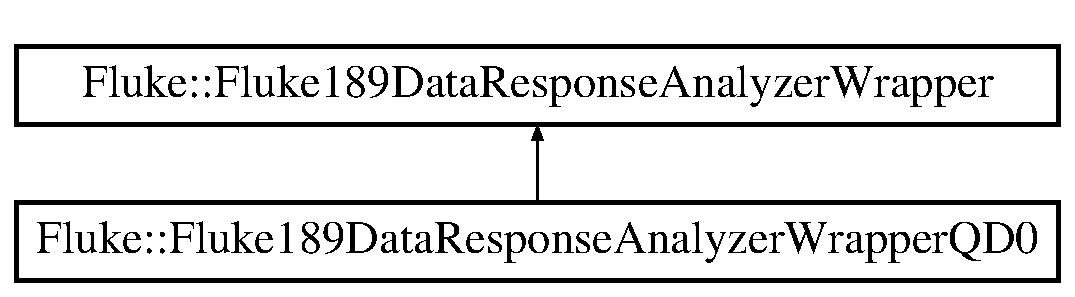
\includegraphics[height=2cm]{classFluke_1_1Fluke189DataResponseAnalyzerWrapper}
\end{center}
\end{figure}
\subsection*{Classes}
\begin{DoxyCompactItemize}
\item 
struct \hyperlink{structFluke_1_1Fluke189DataResponseAnalyzerWrapper_1_1analyzedInfo__t}{analyzedInfo\_\-t}
\end{DoxyCompactItemize}
\subsection*{Public Types}
\begin{DoxyCompactItemize}
\item 
enum \hyperlink{classFluke_1_1Fluke189DataResponseAnalyzerWrapper_a2ec2700a6086ae0ebd9601fe0c0f957a}{ModeSwitchSetting} \{ \par
{\bfseries MS\_\-Unknown} = 0, 
{\bfseries MS\_\-VAC} = 1, 
{\bfseries MS\_\-mVAC} = 2, 
{\bfseries MS\_\-VDC} = 3, 
\par
{\bfseries MS\_\-mVDC} = 4, 
{\bfseries MS\_\-OhmSiemens} = 5, 
{\bfseries MS\_\-CapDiode} = 6, 
{\bfseries MS\_\-Temp} = 7, 
\par
{\bfseries MS\_\-AACmAAC} = 8, 
{\bfseries MS\_\-uAAC} = 9, 
{\bfseries MS\_\-ADCmADC} = 10, 
{\bfseries MS\_\-uADC} = 11, 
\par
{\bfseries MS\_\-VIEWMEM} = 12, 
{\bfseries MS\_\-STUCKBETW2POS} = 99
 \}
\item 
enum \hyperlink{classFluke_1_1Fluke189DataResponseAnalyzerWrapper_ab8e5f2306e4d2ad3d741d273793aaed1}{Unit} \{ \par
{\bfseries AU\_\-None}, 
{\bfseries AU\_\-AC\_\-V}, 
{\bfseries AU\_\-DC\_\-V}, 
{\bfseries AU\_\-ACDC\_\-V}, 
\par
{\bfseries AU\_\-Volts}, 
{\bfseries AU\_\-Ampere}, 
{\bfseries AU\_\-dBm}, 
{\bfseries AU\_\-dB\_\-V}, 
\par
{\bfseries AU\_\-Hz}, 
{\bfseries AU\_\-Seconds}, 
{\bfseries AU\_\-Percent}, 
{\bfseries AU\_\-Ohm}, 
\par
{\bfseries AU\_\-Siemens}, 
{\bfseries AU\_\-Farad}, 
{\bfseries AU\_\-Celsius}, 
{\bfseries AU\_\-Fahrenheit}
 \}
\item 
enum \hyperlink{classFluke_1_1Fluke189DataResponseAnalyzerWrapper_afef24496da239e3613c40ad3582d7adc}{CurrentType} \{ {\bfseries ACT\_\-NoCurrentType}, 
{\bfseries ACT\_\-AlternatingCurrent}, 
{\bfseries ACT\_\-DirectCurrent}, 
{\bfseries ACT\_\-DirectandAlternatingCurrent}
 \}
\item 
enum \hyperlink{classFluke_1_1Fluke189DataResponseAnalyzerWrapper_ada71f6ab32a7b0eb40bb0ed96d7053bc}{Etch} \{ {\bfseries AE\_\-NOT\_\-APPLICABLE}, 
{\bfseries AE\_\-FALLING\_\-ETCH}, 
{\bfseries AE\_\-RISING\_\-ETCH}
 \}
\end{DoxyCompactItemize}
\subsection*{Public Member Functions}
\begin{DoxyCompactItemize}
\item 
\hyperlink{classFluke_1_1Fluke189DataResponseAnalyzerWrapper_af4f891231353edf2c9a20743d3018b1e}{Fluke189DataResponseAnalyzerWrapper} (unsigned int \hyperlink{classFluke_1_1Fluke189DataResponseAnalyzerWrapper_a568ccec1349cc6b278fb0791182bc7b4}{datasetnumber}, void $\ast$\hyperlink{classFluke_1_1Fluke189DataResponseAnalyzerWrapper_aa0096243be3694f7993022733703697a}{currentContainer})
\item 
\hyperlink{structFluke_1_1Fluke189DataResponseAnalyzerWrapper_1_1analyzedInfo__t}{analyzedInfo\_\-t} \hyperlink{classFluke_1_1Fluke189DataResponseAnalyzerWrapper_a2bec1dad601bc993375d358ef77c7e6b}{analyzeQdInfo} (\hyperlink{structFluke_1_1Fluke189_1_1qdInfo__t}{Fluke::Fluke189::qdInfo\_\-t} $\ast$qdInfo)
\item 
std::string \hyperlink{classFluke_1_1Fluke189DataResponseAnalyzerWrapper_ac6af92576728d360cf3e0d462d07dd27}{valueErrorToString} (\hyperlink{classFluke_1_1Fluke189_a5dc0eaffde0a29a64cbcbd50d4178491}{Fluke::Fluke189::ValueError} number)
\item 
virtual bool \hyperlink{classFluke_1_1Fluke189DataResponseAnalyzerWrapper_a831296ad9286753efede158c207adc19}{hasErrorPRIdisplay} (bool reading2)=0
\item 
virtual bool \hyperlink{classFluke_1_1Fluke189DataResponseAnalyzerWrapper_aa78f02012a5f1803c080bae3e6121286}{hasErrorSECdisplay} (bool reading2)=0
\item 
virtual \hyperlink{classFluke_1_1Fluke189_a5dc0eaffde0a29a64cbcbd50d4178491}{Fluke189::ValueError} \hyperlink{classFluke_1_1Fluke189DataResponseAnalyzerWrapper_ad10698c83895619a6fbf251c1256ce11}{get\_\-PRIdisplayError} (bool reading2)=0
\item 
virtual \hyperlink{classFluke_1_1Fluke189_a5dc0eaffde0a29a64cbcbd50d4178491}{Fluke189::ValueError} \hyperlink{classFluke_1_1Fluke189DataResponseAnalyzerWrapper_aaf53f3e129ae21be4abe85bf4998fed5}{get\_\-SECdisplayError} (bool reading2)=0
\item 
virtual \hyperlink{classFluke_1_1Fluke189DataResponseAnalyzerWrapper_a2ec2700a6086ae0ebd9601fe0c0f957a}{ModeSwitchSetting} \hyperlink{classFluke_1_1Fluke189DataResponseAnalyzerWrapper_a18e1b686e50a4cc3a7023c646f66a35c}{get\_\-ModeSwitchSetting} ()=0
\item 
virtual \hyperlink{classFluke_1_1Fluke189DataResponseAnalyzerWrapper_ab8e5f2306e4d2ad3d741d273793aaed1}{Unit} \hyperlink{classFluke_1_1Fluke189DataResponseAnalyzerWrapper_a81fd0f497095dba37f2a614bd35426db}{get\_\-primaryUnit} ()=0
\item 
virtual \hyperlink{classFluke_1_1Fluke189DataResponseAnalyzerWrapper_ab8e5f2306e4d2ad3d741d273793aaed1}{Unit} \hyperlink{classFluke_1_1Fluke189DataResponseAnalyzerWrapper_a8c24a1f3d5abae862ffa06a3a7ac44f1}{get\_\-secondaryUnit} ()=0
\item 
virtual \hyperlink{classFluke_1_1Fluke189DataResponseAnalyzerWrapper_afef24496da239e3613c40ad3582d7adc}{CurrentType} \hyperlink{classFluke_1_1Fluke189DataResponseAnalyzerWrapper_afb7361d6963bb0edd9194ba72a1583df}{get\_\-primaryCurrentType} ()=0
\item 
virtual \hyperlink{classFluke_1_1Fluke189DataResponseAnalyzerWrapper_afef24496da239e3613c40ad3582d7adc}{CurrentType} \hyperlink{classFluke_1_1Fluke189DataResponseAnalyzerWrapper_a21a39a54587e31af04c931b46aa11806}{get\_\-secondaryCurrentType} ()=0
\item 
virtual \hyperlink{classFluke_1_1Fluke189DataResponseAnalyzerWrapper_ada71f6ab32a7b0eb40bb0ed96d7053bc}{Etch} \hyperlink{classFluke_1_1Fluke189DataResponseAnalyzerWrapper_a258e56c1ff27b8aae648940599d3b475}{get\_\-EtchInfo} ()=0
\end{DoxyCompactItemize}
\subsection*{Protected Attributes}
\begin{DoxyCompactItemize}
\item 
\hypertarget{classFluke_1_1Fluke189DataResponseAnalyzerWrapper_a568ccec1349cc6b278fb0791182bc7b4}{
unsigned int \hyperlink{classFluke_1_1Fluke189DataResponseAnalyzerWrapper_a568ccec1349cc6b278fb0791182bc7b4}{datasetnumber}}
\label{classFluke_1_1Fluke189DataResponseAnalyzerWrapper_a568ccec1349cc6b278fb0791182bc7b4}

\begin{DoxyCompactList}\small\item\em helds the number of the current data set \item\end{DoxyCompactList}\item 
\hypertarget{classFluke_1_1Fluke189DataResponseAnalyzerWrapper_aa0096243be3694f7993022733703697a}{
void $\ast$ \hyperlink{classFluke_1_1Fluke189DataResponseAnalyzerWrapper_aa0096243be3694f7993022733703697a}{currentContainer}}
\label{classFluke_1_1Fluke189DataResponseAnalyzerWrapper_aa0096243be3694f7993022733703697a}

\begin{DoxyCompactList}\small\item\em helds the address of a supported container type \item\end{DoxyCompactList}\end{DoxyCompactItemize}
\subsection*{Friends}
\begin{DoxyCompactItemize}
\item 
\hypertarget{classFluke_1_1Fluke189DataResponseAnalyzerWrapper_a268eb1bf9fac46f61af93c2c1e309713}{
class {\bfseries Fluke189DataResponseAnalyzer}}
\label{classFluke_1_1Fluke189DataResponseAnalyzerWrapper_a268eb1bf9fac46f61af93c2c1e309713}

\end{DoxyCompactItemize}


\subsection{Detailed Description}
This Wrapper is the superclass for the different data sets. The class to creating a subclass of this is only used to store the current SerialResponseContainer and its type. The member functions of this Wrapper are called by Fluke189ResponseAnalyser::operator\mbox{[}$\,$\mbox{]}(unsigned int) This class is a superclass so it can not be constructed. 

\subsection{Member Enumeration Documentation}
\hypertarget{classFluke_1_1Fluke189DataResponseAnalyzerWrapper_afef24496da239e3613c40ad3582d7adc}{
\index{Fluke::Fluke189DataResponseAnalyzerWrapper@{Fluke::Fluke189DataResponseAnalyzerWrapper}!CurrentType@{CurrentType}}
\index{CurrentType@{CurrentType}!Fluke::Fluke189DataResponseAnalyzerWrapper@{Fluke::Fluke189DataResponseAnalyzerWrapper}}
\subsubsection[{CurrentType}]{\setlength{\rightskip}{0pt plus 5cm}enum {\bf Fluke::Fluke189DataResponseAnalyzerWrapper::CurrentType}}}
\label{classFluke_1_1Fluke189DataResponseAnalyzerWrapper_afef24496da239e3613c40ad3582d7adc}
Voltage Types (AC, DC, AC+DC) \hypertarget{classFluke_1_1Fluke189DataResponseAnalyzerWrapper_ada71f6ab32a7b0eb40bb0ed96d7053bc}{
\index{Fluke::Fluke189DataResponseAnalyzerWrapper@{Fluke::Fluke189DataResponseAnalyzerWrapper}!Etch@{Etch}}
\index{Etch@{Etch}!Fluke::Fluke189DataResponseAnalyzerWrapper@{Fluke::Fluke189DataResponseAnalyzerWrapper}}
\subsubsection[{Etch}]{\setlength{\rightskip}{0pt plus 5cm}enum {\bf Fluke::Fluke189DataResponseAnalyzerWrapper::Etch}}}
\label{classFluke_1_1Fluke189DataResponseAnalyzerWrapper_ada71f6ab32a7b0eb40bb0ed96d7053bc}
Etch information (falling etch, rising etch, not applicable) \hypertarget{classFluke_1_1Fluke189DataResponseAnalyzerWrapper_a2ec2700a6086ae0ebd9601fe0c0f957a}{
\index{Fluke::Fluke189DataResponseAnalyzerWrapper@{Fluke::Fluke189DataResponseAnalyzerWrapper}!ModeSwitchSetting@{ModeSwitchSetting}}
\index{ModeSwitchSetting@{ModeSwitchSetting}!Fluke::Fluke189DataResponseAnalyzerWrapper@{Fluke::Fluke189DataResponseAnalyzerWrapper}}
\subsubsection[{ModeSwitchSetting}]{\setlength{\rightskip}{0pt plus 5cm}enum {\bf Fluke::Fluke189DataResponseAnalyzerWrapper::ModeSwitchSetting}}}
\label{classFluke_1_1Fluke189DataResponseAnalyzerWrapper_a2ec2700a6086ae0ebd9601fe0c0f957a}
Return values of the analysis for the position of the mode switch \hypertarget{classFluke_1_1Fluke189DataResponseAnalyzerWrapper_ab8e5f2306e4d2ad3d741d273793aaed1}{
\index{Fluke::Fluke189DataResponseAnalyzerWrapper@{Fluke::Fluke189DataResponseAnalyzerWrapper}!Unit@{Unit}}
\index{Unit@{Unit}!Fluke::Fluke189DataResponseAnalyzerWrapper@{Fluke::Fluke189DataResponseAnalyzerWrapper}}
\subsubsection[{Unit}]{\setlength{\rightskip}{0pt plus 5cm}enum {\bf Fluke::Fluke189DataResponseAnalyzerWrapper::Unit}}}
\label{classFluke_1_1Fluke189DataResponseAnalyzerWrapper_ab8e5f2306e4d2ad3d741d273793aaed1}
Returned units by analysis 

\subsection{Constructor \& Destructor Documentation}
\hypertarget{classFluke_1_1Fluke189DataResponseAnalyzerWrapper_af4f891231353edf2c9a20743d3018b1e}{
\index{Fluke::Fluke189DataResponseAnalyzerWrapper@{Fluke::Fluke189DataResponseAnalyzerWrapper}!Fluke189DataResponseAnalyzerWrapper@{Fluke189DataResponseAnalyzerWrapper}}
\index{Fluke189DataResponseAnalyzerWrapper@{Fluke189DataResponseAnalyzerWrapper}!Fluke::Fluke189DataResponseAnalyzerWrapper@{Fluke::Fluke189DataResponseAnalyzerWrapper}}
\subsubsection[{Fluke189DataResponseAnalyzerWrapper}]{\setlength{\rightskip}{0pt plus 5cm}Fluke::Fluke189DataResponseAnalyzerWrapper::Fluke189DataResponseAnalyzerWrapper (unsigned int {\em datasetnumber}, \/  void $\ast$ {\em currentContainer})\hspace{0.3cm}{\ttfamily  \mbox{[}inline\mbox{]}}}}
\label{classFluke_1_1Fluke189DataResponseAnalyzerWrapper_af4f891231353edf2c9a20743d3018b1e}
Constructor param\mbox{[}in\mbox{]} datasetnumber Number of the data set to be edited param\mbox{[}in\mbox{]} currentContainer Points to the current data set container 

\subsection{Member Function Documentation}
\hypertarget{classFluke_1_1Fluke189DataResponseAnalyzerWrapper_a2bec1dad601bc993375d358ef77c7e6b}{
\index{Fluke::Fluke189DataResponseAnalyzerWrapper@{Fluke::Fluke189DataResponseAnalyzerWrapper}!analyzeQdInfo@{analyzeQdInfo}}
\index{analyzeQdInfo@{analyzeQdInfo}!Fluke::Fluke189DataResponseAnalyzerWrapper@{Fluke::Fluke189DataResponseAnalyzerWrapper}}
\subsubsection[{analyzeQdInfo}]{\setlength{\rightskip}{0pt plus 5cm}{\bf Fluke189DataResponseAnalyzerWrapper::analyzedInfo\_\-t} Fluke::Fluke189DataResponseAnalyzerWrapper::analyzeQdInfo ({\bf Fluke::Fluke189::qdInfo\_\-t} $\ast$ {\em qdInfo})}}
\label{classFluke_1_1Fluke189DataResponseAnalyzerWrapper_a2bec1dad601bc993375d358ef77c7e6b}
Returns a struct with additional information created by analyzing qdInfo.\par
 It containes the primary and secondary units, current types and shows if the multimeter is currently in logging or viewmem mode\par
 {\bfseries ATTENTION:} Currently its not possible to be sure that the multimeter is in viewmem. If \char`\"{}Clr?\char`\"{} is displayed the return value will fall back to the mode which was selected when the log/save was stored. \begin{Desc}
\item[\hyperlink{todo__todo000022}{Todo}]find a fix for the recognize viemem correctly bug \end{Desc}

\begin{DoxyParams}{Parameters}
\item[\mbox{$\leftarrow$} {\em qdInfo}]Struct containing setup for the current reading \end{DoxyParams}
\begin{DoxyReturn}{Returns}
Struct containing additional information. 
\end{DoxyReturn}
\hypertarget{classFluke_1_1Fluke189DataResponseAnalyzerWrapper_a258e56c1ff27b8aae648940599d3b475}{
\index{Fluke::Fluke189DataResponseAnalyzerWrapper@{Fluke::Fluke189DataResponseAnalyzerWrapper}!get\_\-EtchInfo@{get\_\-EtchInfo}}
\index{get\_\-EtchInfo@{get\_\-EtchInfo}!Fluke::Fluke189DataResponseAnalyzerWrapper@{Fluke::Fluke189DataResponseAnalyzerWrapper}}
\subsubsection[{get\_\-EtchInfo}]{\setlength{\rightskip}{0pt plus 5cm}virtual {\bf Etch} Fluke::Fluke189DataResponseAnalyzerWrapper::get\_\-EtchInfo ()\hspace{0.3cm}{\ttfamily  \mbox{[}pure virtual\mbox{]}}}}
\label{classFluke_1_1Fluke189DataResponseAnalyzerWrapper_a258e56c1ff27b8aae648940599d3b475}
Get current etch information (rising, falling, not applicable) \begin{DoxyReturn}{Returns}
etch information according to \hyperlink{classFluke_1_1Fluke189DataResponseAnalyzerWrapper_ada71f6ab32a7b0eb40bb0ed96d7053bc}{Fluke189DataResponseAnalyzerWrapper::Etch} 
\end{DoxyReturn}


Implemented in \hyperlink{classFluke_1_1Fluke189DataResponseAnalyzerWrapperQD0_a8a50c55ebd21461e4c934a1eb4b07641}{Fluke::Fluke189DataResponseAnalyzerWrapperQD0}.\hypertarget{classFluke_1_1Fluke189DataResponseAnalyzerWrapper_a18e1b686e50a4cc3a7023c646f66a35c}{
\index{Fluke::Fluke189DataResponseAnalyzerWrapper@{Fluke::Fluke189DataResponseAnalyzerWrapper}!get\_\-ModeSwitchSetting@{get\_\-ModeSwitchSetting}}
\index{get\_\-ModeSwitchSetting@{get\_\-ModeSwitchSetting}!Fluke::Fluke189DataResponseAnalyzerWrapper@{Fluke::Fluke189DataResponseAnalyzerWrapper}}
\subsubsection[{get\_\-ModeSwitchSetting}]{\setlength{\rightskip}{0pt plus 5cm}virtual {\bf ModeSwitchSetting} Fluke::Fluke189DataResponseAnalyzerWrapper::get\_\-ModeSwitchSetting ()\hspace{0.3cm}{\ttfamily  \mbox{[}pure virtual\mbox{]}}}}
\label{classFluke_1_1Fluke189DataResponseAnalyzerWrapper_a18e1b686e50a4cc3a7023c646f66a35c}
Shows the current mode switch setting \begin{DoxyReturn}{Returns}
Number of mode switch or 0 when stuck between two positions 
\end{DoxyReturn}


Implemented in \hyperlink{classFluke_1_1Fluke189DataResponseAnalyzerWrapperQD0_ad28a17399ffe6a926990aafd5a1891d3}{Fluke::Fluke189DataResponseAnalyzerWrapperQD0}.\hypertarget{classFluke_1_1Fluke189DataResponseAnalyzerWrapper_ad10698c83895619a6fbf251c1256ce11}{
\index{Fluke::Fluke189DataResponseAnalyzerWrapper@{Fluke::Fluke189DataResponseAnalyzerWrapper}!get\_\-PRIdisplayError@{get\_\-PRIdisplayError}}
\index{get\_\-PRIdisplayError@{get\_\-PRIdisplayError}!Fluke::Fluke189DataResponseAnalyzerWrapper@{Fluke::Fluke189DataResponseAnalyzerWrapper}}
\subsubsection[{get\_\-PRIdisplayError}]{\setlength{\rightskip}{0pt plus 5cm}virtual {\bf Fluke189::ValueError} Fluke::Fluke189DataResponseAnalyzerWrapper::get\_\-PRIdisplayError (bool {\em reading2})\hspace{0.3cm}{\ttfamily  \mbox{[}pure virtual\mbox{]}}}}
\label{classFluke_1_1Fluke189DataResponseAnalyzerWrapper_ad10698c83895619a6fbf251c1256ce11}
This function returns the ErrorValue of the primary reading 
\begin{DoxyParams}{Parameters}
\item[\mbox{$\leftarrow$} {\em reading2}]If {\bfseries true} second primary reading will be used. \end{DoxyParams}
\begin{DoxyReturn}{Returns}
Error numbers according to \hyperlink{classFluke_1_1Fluke189_a5dc0eaffde0a29a64cbcbd50d4178491}{Fluke189::ValueError} 
\end{DoxyReturn}


Implemented in \hyperlink{classFluke_1_1Fluke189DataResponseAnalyzerWrapperQD0_a4a3343d00db4cda2bf021074f2cfdadc}{Fluke::Fluke189DataResponseAnalyzerWrapperQD0}.\hypertarget{classFluke_1_1Fluke189DataResponseAnalyzerWrapper_afb7361d6963bb0edd9194ba72a1583df}{
\index{Fluke::Fluke189DataResponseAnalyzerWrapper@{Fluke::Fluke189DataResponseAnalyzerWrapper}!get\_\-primaryCurrentType@{get\_\-primaryCurrentType}}
\index{get\_\-primaryCurrentType@{get\_\-primaryCurrentType}!Fluke::Fluke189DataResponseAnalyzerWrapper@{Fluke::Fluke189DataResponseAnalyzerWrapper}}
\subsubsection[{get\_\-primaryCurrentType}]{\setlength{\rightskip}{0pt plus 5cm}virtual {\bf CurrentType} Fluke::Fluke189DataResponseAnalyzerWrapper::get\_\-primaryCurrentType ()\hspace{0.3cm}{\ttfamily  \mbox{[}pure virtual\mbox{]}}}}
\label{classFluke_1_1Fluke189DataResponseAnalyzerWrapper_afb7361d6963bb0edd9194ba72a1583df}
Get current type of the primary reading (AC, DC, AC+DC, not applicable) \begin{DoxyReturn}{Returns}
CurrentType according to \hyperlink{classFluke_1_1Fluke189DataResponseAnalyzerWrapper_afef24496da239e3613c40ad3582d7adc}{Fluke189DataResponseAnalyzerWrapper::CurrentType} 
\end{DoxyReturn}


Implemented in \hyperlink{classFluke_1_1Fluke189DataResponseAnalyzerWrapperQD0_acffb9af55e2d690060ef210977c3c933}{Fluke::Fluke189DataResponseAnalyzerWrapperQD0}.\hypertarget{classFluke_1_1Fluke189DataResponseAnalyzerWrapper_a81fd0f497095dba37f2a614bd35426db}{
\index{Fluke::Fluke189DataResponseAnalyzerWrapper@{Fluke::Fluke189DataResponseAnalyzerWrapper}!get\_\-primaryUnit@{get\_\-primaryUnit}}
\index{get\_\-primaryUnit@{get\_\-primaryUnit}!Fluke::Fluke189DataResponseAnalyzerWrapper@{Fluke::Fluke189DataResponseAnalyzerWrapper}}
\subsubsection[{get\_\-primaryUnit}]{\setlength{\rightskip}{0pt plus 5cm}virtual {\bf Unit} Fluke::Fluke189DataResponseAnalyzerWrapper::get\_\-primaryUnit ()\hspace{0.3cm}{\ttfamily  \mbox{[}pure virtual\mbox{]}}}}
\label{classFluke_1_1Fluke189DataResponseAnalyzerWrapper_a81fd0f497095dba37f2a614bd35426db}
Get physical unit of the primary reading. \begin{DoxyReturn}{Returns}
Physical unit of the current reading according to Fluke189DataResponseAnalyzerWrapper::enum Unit 
\end{DoxyReturn}


Implemented in \hyperlink{classFluke_1_1Fluke189DataResponseAnalyzerWrapperQD0_af71dd62d9f81866ad3cb96c580754329}{Fluke::Fluke189DataResponseAnalyzerWrapperQD0}.\hypertarget{classFluke_1_1Fluke189DataResponseAnalyzerWrapper_aaf53f3e129ae21be4abe85bf4998fed5}{
\index{Fluke::Fluke189DataResponseAnalyzerWrapper@{Fluke::Fluke189DataResponseAnalyzerWrapper}!get\_\-SECdisplayError@{get\_\-SECdisplayError}}
\index{get\_\-SECdisplayError@{get\_\-SECdisplayError}!Fluke::Fluke189DataResponseAnalyzerWrapper@{Fluke::Fluke189DataResponseAnalyzerWrapper}}
\subsubsection[{get\_\-SECdisplayError}]{\setlength{\rightskip}{0pt plus 5cm}virtual {\bf Fluke189::ValueError} Fluke::Fluke189DataResponseAnalyzerWrapper::get\_\-SECdisplayError (bool {\em reading2})\hspace{0.3cm}{\ttfamily  \mbox{[}pure virtual\mbox{]}}}}
\label{classFluke_1_1Fluke189DataResponseAnalyzerWrapper_aaf53f3e129ae21be4abe85bf4998fed5}
This function returns the ErrorValue of the secondary reading 
\begin{DoxyParams}{Parameters}
\item[\mbox{$\leftarrow$} {\em reading2}]If {\bfseries true} second secondary reading will be used (QD0 only). \end{DoxyParams}
\begin{DoxyReturn}{Returns}
Error numbers according to \hyperlink{classFluke_1_1Fluke189_a5dc0eaffde0a29a64cbcbd50d4178491}{Fluke189::ValueError} 
\end{DoxyReturn}


Implemented in \hyperlink{classFluke_1_1Fluke189DataResponseAnalyzerWrapperQD0_a72e91f8c908b7fa8ce541308a53ff696}{Fluke::Fluke189DataResponseAnalyzerWrapperQD0}.\hypertarget{classFluke_1_1Fluke189DataResponseAnalyzerWrapper_a21a39a54587e31af04c931b46aa11806}{
\index{Fluke::Fluke189DataResponseAnalyzerWrapper@{Fluke::Fluke189DataResponseAnalyzerWrapper}!get\_\-secondaryCurrentType@{get\_\-secondaryCurrentType}}
\index{get\_\-secondaryCurrentType@{get\_\-secondaryCurrentType}!Fluke::Fluke189DataResponseAnalyzerWrapper@{Fluke::Fluke189DataResponseAnalyzerWrapper}}
\subsubsection[{get\_\-secondaryCurrentType}]{\setlength{\rightskip}{0pt plus 5cm}virtual {\bf CurrentType} Fluke::Fluke189DataResponseAnalyzerWrapper::get\_\-secondaryCurrentType ()\hspace{0.3cm}{\ttfamily  \mbox{[}pure virtual\mbox{]}}}}
\label{classFluke_1_1Fluke189DataResponseAnalyzerWrapper_a21a39a54587e31af04c931b46aa11806}
Get current type of the secondary reading (AC, DC, AC+DC, not applicable) \begin{DoxyReturn}{Returns}
CurrentType according to \hyperlink{classFluke_1_1Fluke189DataResponseAnalyzerWrapper_afef24496da239e3613c40ad3582d7adc}{Fluke189DataResponseAnalyzerWrapper::CurrentType} 
\end{DoxyReturn}


Implemented in \hyperlink{classFluke_1_1Fluke189DataResponseAnalyzerWrapperQD0_aa46ac22750b412df37ae24db84fab138}{Fluke::Fluke189DataResponseAnalyzerWrapperQD0}.\hypertarget{classFluke_1_1Fluke189DataResponseAnalyzerWrapper_a8c24a1f3d5abae862ffa06a3a7ac44f1}{
\index{Fluke::Fluke189DataResponseAnalyzerWrapper@{Fluke::Fluke189DataResponseAnalyzerWrapper}!get\_\-secondaryUnit@{get\_\-secondaryUnit}}
\index{get\_\-secondaryUnit@{get\_\-secondaryUnit}!Fluke::Fluke189DataResponseAnalyzerWrapper@{Fluke::Fluke189DataResponseAnalyzerWrapper}}
\subsubsection[{get\_\-secondaryUnit}]{\setlength{\rightskip}{0pt plus 5cm}virtual {\bf Unit} Fluke::Fluke189DataResponseAnalyzerWrapper::get\_\-secondaryUnit ()\hspace{0.3cm}{\ttfamily  \mbox{[}pure virtual\mbox{]}}}}
\label{classFluke_1_1Fluke189DataResponseAnalyzerWrapper_a8c24a1f3d5abae862ffa06a3a7ac44f1}
Get physical unit of the secondary reading. \begin{DoxyReturn}{Returns}
Physical unit of the current reading according to Fluke189DataResponseAnalyzerWrapper::enum Unit 
\end{DoxyReturn}


Implemented in \hyperlink{classFluke_1_1Fluke189DataResponseAnalyzerWrapperQD0_a3f1bdb92d10f341c8b22fa8ee95600b5}{Fluke::Fluke189DataResponseAnalyzerWrapperQD0}.\hypertarget{classFluke_1_1Fluke189DataResponseAnalyzerWrapper_a831296ad9286753efede158c207adc19}{
\index{Fluke::Fluke189DataResponseAnalyzerWrapper@{Fluke::Fluke189DataResponseAnalyzerWrapper}!hasErrorPRIdisplay@{hasErrorPRIdisplay}}
\index{hasErrorPRIdisplay@{hasErrorPRIdisplay}!Fluke::Fluke189DataResponseAnalyzerWrapper@{Fluke::Fluke189DataResponseAnalyzerWrapper}}
\subsubsection[{hasErrorPRIdisplay}]{\setlength{\rightskip}{0pt plus 5cm}virtual bool Fluke::Fluke189DataResponseAnalyzerWrapper::hasErrorPRIdisplay (bool {\em reading2})\hspace{0.3cm}{\ttfamily  \mbox{[}pure virtual\mbox{]}}}}
\label{classFluke_1_1Fluke189DataResponseAnalyzerWrapper_a831296ad9286753efede158c207adc19}
Checks if a error in measurement is present in the current primary reading 
\begin{DoxyParams}{Parameters}
\item[\mbox{$\leftarrow$} {\em reading2}]If {\bfseries true} second primary reading will be used. \end{DoxyParams}
\begin{DoxyReturn}{Returns}
{\bfseries true} if the primary display value has an error 
\end{DoxyReturn}


Implemented in \hyperlink{classFluke_1_1Fluke189DataResponseAnalyzerWrapperQD0_aeffd54445d733f8b149c5918589e5b9e}{Fluke::Fluke189DataResponseAnalyzerWrapperQD0}.\hypertarget{classFluke_1_1Fluke189DataResponseAnalyzerWrapper_aa78f02012a5f1803c080bae3e6121286}{
\index{Fluke::Fluke189DataResponseAnalyzerWrapper@{Fluke::Fluke189DataResponseAnalyzerWrapper}!hasErrorSECdisplay@{hasErrorSECdisplay}}
\index{hasErrorSECdisplay@{hasErrorSECdisplay}!Fluke::Fluke189DataResponseAnalyzerWrapper@{Fluke::Fluke189DataResponseAnalyzerWrapper}}
\subsubsection[{hasErrorSECdisplay}]{\setlength{\rightskip}{0pt plus 5cm}virtual bool Fluke::Fluke189DataResponseAnalyzerWrapper::hasErrorSECdisplay (bool {\em reading2})\hspace{0.3cm}{\ttfamily  \mbox{[}pure virtual\mbox{]}}}}
\label{classFluke_1_1Fluke189DataResponseAnalyzerWrapper_aa78f02012a5f1803c080bae3e6121286}
Checks if a error in measurement is present in the current secondary reading 
\begin{DoxyParams}{Parameters}
\item[\mbox{$\leftarrow$} {\em reading2}]If {\bfseries true} second primary reading will be used. \end{DoxyParams}
\begin{DoxyReturn}{Returns}
{\bfseries true} if the secondary display value has an error 
\end{DoxyReturn}


Implemented in \hyperlink{classFluke_1_1Fluke189DataResponseAnalyzerWrapperQD0_a97829a1943b858fd09c4fef1d6d61420}{Fluke::Fluke189DataResponseAnalyzerWrapperQD0}.\hypertarget{classFluke_1_1Fluke189DataResponseAnalyzerWrapper_ac6af92576728d360cf3e0d462d07dd27}{
\index{Fluke::Fluke189DataResponseAnalyzerWrapper@{Fluke::Fluke189DataResponseAnalyzerWrapper}!valueErrorToString@{valueErrorToString}}
\index{valueErrorToString@{valueErrorToString}!Fluke::Fluke189DataResponseAnalyzerWrapper@{Fluke::Fluke189DataResponseAnalyzerWrapper}}
\subsubsection[{valueErrorToString}]{\setlength{\rightskip}{0pt plus 5cm}std::string Fluke::Fluke189DataResponseAnalyzerWrapper::valueErrorToString ({\bf Fluke::Fluke189::ValueError} {\em number})}}
\label{classFluke_1_1Fluke189DataResponseAnalyzerWrapper_ac6af92576728d360cf3e0d462d07dd27}
Returns the error string according to the ValueError number 
\begin{DoxyParams}{Parameters}
\item[\mbox{$\leftarrow$} {\em number}]ValueError \end{DoxyParams}
\begin{DoxyReturn}{Returns}
A human readable error string 
\end{DoxyReturn}


The documentation for this class was generated from the following files:\begin{DoxyCompactItemize}
\item 
src/Fluke189.hpp\item 
src/Fluke189.cpp\end{DoxyCompactItemize}

\hypertarget{classFluke_1_1Fluke189DataResponseAnalyzerWrapperQD0}{
\section{Fluke::Fluke189DataResponseAnalyzerWrapperQD0 Class Reference}
\label{classFluke_1_1Fluke189DataResponseAnalyzerWrapperQD0}\index{Fluke::Fluke189DataResponseAnalyzerWrapperQD0@{Fluke::Fluke189DataResponseAnalyzerWrapperQD0}}
}


{\ttfamily \#include $<$Fluke189.hpp$>$}Inheritance diagram for Fluke::Fluke189DataResponseAnalyzerWrapperQD0::\begin{figure}[H]
\begin{center}
\leavevmode
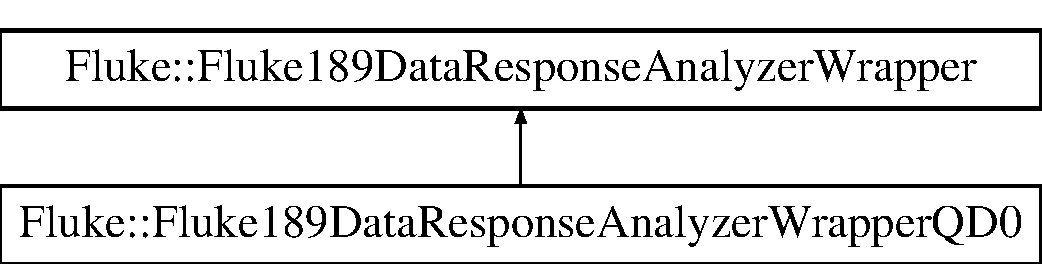
\includegraphics[height=2cm]{classFluke_1_1Fluke189DataResponseAnalyzerWrapperQD0}
\end{center}
\end{figure}
\subsection*{Public Member Functions}
\begin{DoxyCompactItemize}
\item 
\hyperlink{structFluke_1_1Fluke189DataResponseAnalyzerWrapper_1_1analyzedInfo__t}{analyzedInfo\_\-t} \hyperlink{classFluke_1_1Fluke189DataResponseAnalyzerWrapperQD0_af6e15c77a255dbebaaeb61e6848e8b42}{getAnalyzedInfoStruct} ()
\item 
bool \hyperlink{classFluke_1_1Fluke189DataResponseAnalyzerWrapperQD0_a173f4602b71d7d415e11aa1f1826d3f0}{hasErrorPRIdisplay} ()
\item 
bool \hyperlink{classFluke_1_1Fluke189DataResponseAnalyzerWrapperQD0_aad8855dc897cc83a4a7b4df79657a724}{hasErrorSECdisplay} ()
\item 
\hyperlink{classFluke_1_1Fluke189DataResponseAnalyzerWrapper_a5e26140c615bf0b73788f665a7bec9c7}{DispError} \hyperlink{classFluke_1_1Fluke189DataResponseAnalyzerWrapperQD0_a92b0a7a3c0cfd671f86df8e8b61aebb8}{get\_\-PRIdisplayError} ()
\item 
\hyperlink{classFluke_1_1Fluke189DataResponseAnalyzerWrapper_a5e26140c615bf0b73788f665a7bec9c7}{DispError} \hyperlink{classFluke_1_1Fluke189DataResponseAnalyzerWrapperQD0_a26e5925f4ca96aeea4115c44aa8ed1a8}{get\_\-SECdisplayError} ()
\item 
\hyperlink{classFluke_1_1Fluke189DataResponseAnalyzerWrapper_a2ec2700a6086ae0ebd9601fe0c0f957a}{ModeSwitchSetting} \hyperlink{classFluke_1_1Fluke189DataResponseAnalyzerWrapperQD0_ad28a17399ffe6a926990aafd5a1891d3}{get\_\-ModeSwitchSetting} ()
\item 
\hyperlink{classFluke_1_1Fluke189DataResponseAnalyzerWrapper_ab8e5f2306e4d2ad3d741d273793aaed1}{Unit} \hyperlink{classFluke_1_1Fluke189DataResponseAnalyzerWrapperQD0_af71dd62d9f81866ad3cb96c580754329}{get\_\-primaryUnit} ()
\item 
\hyperlink{classFluke_1_1Fluke189DataResponseAnalyzerWrapper_ab8e5f2306e4d2ad3d741d273793aaed1}{Unit} \hyperlink{classFluke_1_1Fluke189DataResponseAnalyzerWrapperQD0_a3f1bdb92d10f341c8b22fa8ee95600b5}{get\_\-secondaryUnit} ()
\item 
\hyperlink{classFluke_1_1Fluke189DataResponseAnalyzerWrapper_afef24496da239e3613c40ad3582d7adc}{CurrentType} \hyperlink{classFluke_1_1Fluke189DataResponseAnalyzerWrapperQD0_acffb9af55e2d690060ef210977c3c933}{get\_\-primaryCurrentType} ()
\item 
\hyperlink{classFluke_1_1Fluke189DataResponseAnalyzerWrapper_afef24496da239e3613c40ad3582d7adc}{CurrentType} \hyperlink{classFluke_1_1Fluke189DataResponseAnalyzerWrapperQD0_aa46ac22750b412df37ae24db84fab138}{get\_\-secondaryCurrentType} ()
\item 
\hyperlink{classFluke_1_1Fluke189DataResponseAnalyzerWrapper_ada71f6ab32a7b0eb40bb0ed96d7053bc}{Etch} \hyperlink{classFluke_1_1Fluke189DataResponseAnalyzerWrapperQD0_a8a50c55ebd21461e4c934a1eb4b07641}{get\_\-EtchInfo} ()
\item 
std::string \hyperlink{classFluke_1_1Fluke189DataResponseAnalyzerWrapperQD0_af0968b6176ba724d21a89547147f9be5}{getPrimaryUnitSymbol} ()
\item 
std::string \hyperlink{classFluke_1_1Fluke189DataResponseAnalyzerWrapperQD0_af7a5731fbbd6ac2a7ab2a8d0a9f2ffe6}{getSecondaryUnitSymbol} ()
\end{DoxyCompactItemize}
\subsection*{Friends}
\begin{DoxyCompactItemize}
\item 
\hypertarget{classFluke_1_1Fluke189DataResponseAnalyzerWrapperQD0_a268eb1bf9fac46f61af93c2c1e309713}{
class {\bfseries Fluke189DataResponseAnalyzer}}
\label{classFluke_1_1Fluke189DataResponseAnalyzerWrapperQD0_a268eb1bf9fac46f61af93c2c1e309713}

\end{DoxyCompactItemize}


\subsection{Detailed Description}
This is the subclass which holds the real functions for analyzing the response of QD0 command Can only be constructed from Fluke189ResponseAnalyser(private constructor) The deconstruction is also done by Fluke189ResponseAnalyser (private destructor) 

\subsection{Member Function Documentation}
\hypertarget{classFluke_1_1Fluke189DataResponseAnalyzerWrapperQD0_a8a50c55ebd21461e4c934a1eb4b07641}{
\index{Fluke::Fluke189DataResponseAnalyzerWrapperQD0@{Fluke::Fluke189DataResponseAnalyzerWrapperQD0}!get\_\-EtchInfo@{get\_\-EtchInfo}}
\index{get\_\-EtchInfo@{get\_\-EtchInfo}!Fluke::Fluke189DataResponseAnalyzerWrapperQD0@{Fluke::Fluke189DataResponseAnalyzerWrapperQD0}}
\subsubsection[{get\_\-EtchInfo}]{\setlength{\rightskip}{0pt plus 5cm}{\bf Fluke189DataResponseAnalyzerWrapper::Etch} Fluke::Fluke189DataResponseAnalyzerWrapperQD0::get\_\-EtchInfo ()\hspace{0.3cm}{\ttfamily  \mbox{[}virtual\mbox{]}}}}
\label{classFluke_1_1Fluke189DataResponseAnalyzerWrapperQD0_a8a50c55ebd21461e4c934a1eb4b07641}
Get current etch information (rising, falling, not applicable) \begin{DoxyReturn}{Returns}
etch information according to enum \hyperlink{classFluke_1_1Fluke189DataResponseAnalyzerWrapper_ada71f6ab32a7b0eb40bb0ed96d7053bc}{Fluke189DataResponseAnalyzerWrapper::Etch} 
\end{DoxyReturn}


Implements \hyperlink{classFluke_1_1Fluke189DataResponseAnalyzerWrapper_a258e56c1ff27b8aae648940599d3b475}{Fluke::Fluke189DataResponseAnalyzerWrapper}.\hypertarget{classFluke_1_1Fluke189DataResponseAnalyzerWrapperQD0_ad28a17399ffe6a926990aafd5a1891d3}{
\index{Fluke::Fluke189DataResponseAnalyzerWrapperQD0@{Fluke::Fluke189DataResponseAnalyzerWrapperQD0}!get\_\-ModeSwitchSetting@{get\_\-ModeSwitchSetting}}
\index{get\_\-ModeSwitchSetting@{get\_\-ModeSwitchSetting}!Fluke::Fluke189DataResponseAnalyzerWrapperQD0@{Fluke::Fluke189DataResponseAnalyzerWrapperQD0}}
\subsubsection[{get\_\-ModeSwitchSetting}]{\setlength{\rightskip}{0pt plus 5cm}{\bf Fluke189DataResponseAnalyzerWrapper::ModeSwitchSetting} Fluke::Fluke189DataResponseAnalyzerWrapperQD0::get\_\-ModeSwitchSetting ()\hspace{0.3cm}{\ttfamily  \mbox{[}virtual\mbox{]}}}}
\label{classFluke_1_1Fluke189DataResponseAnalyzerWrapperQD0_ad28a17399ffe6a926990aafd5a1891d3}
Get the current mode switch setting \begin{DoxyReturn}{Returns}
Number of mode switch or 0 when stuck between two positions 
\end{DoxyReturn}


Implements \hyperlink{classFluke_1_1Fluke189DataResponseAnalyzerWrapper_a18e1b686e50a4cc3a7023c646f66a35c}{Fluke::Fluke189DataResponseAnalyzerWrapper}.\hypertarget{classFluke_1_1Fluke189DataResponseAnalyzerWrapperQD0_a92b0a7a3c0cfd671f86df8e8b61aebb8}{
\index{Fluke::Fluke189DataResponseAnalyzerWrapperQD0@{Fluke::Fluke189DataResponseAnalyzerWrapperQD0}!get\_\-PRIdisplayError@{get\_\-PRIdisplayError}}
\index{get\_\-PRIdisplayError@{get\_\-PRIdisplayError}!Fluke::Fluke189DataResponseAnalyzerWrapperQD0@{Fluke::Fluke189DataResponseAnalyzerWrapperQD0}}
\subsubsection[{get\_\-PRIdisplayError}]{\setlength{\rightskip}{0pt plus 5cm}{\bf Fluke189DataResponseAnalyzerWrapper::DispError} Fluke::Fluke189DataResponseAnalyzerWrapperQD0::get\_\-PRIdisplayError ()\hspace{0.3cm}{\ttfamily  \mbox{[}virtual\mbox{]}}}}
\label{classFluke_1_1Fluke189DataResponseAnalyzerWrapperQD0_a92b0a7a3c0cfd671f86df8e8b61aebb8}
This function returns the ErrorValue of the primary reading \begin{DoxyReturn}{Returns}
Error numbers according to DispError 
\end{DoxyReturn}


Implements \hyperlink{classFluke_1_1Fluke189DataResponseAnalyzerWrapper_ae6b5bf434d9600f4178650d66922a3aa}{Fluke::Fluke189DataResponseAnalyzerWrapper}.\hypertarget{classFluke_1_1Fluke189DataResponseAnalyzerWrapperQD0_acffb9af55e2d690060ef210977c3c933}{
\index{Fluke::Fluke189DataResponseAnalyzerWrapperQD0@{Fluke::Fluke189DataResponseAnalyzerWrapperQD0}!get\_\-primaryCurrentType@{get\_\-primaryCurrentType}}
\index{get\_\-primaryCurrentType@{get\_\-primaryCurrentType}!Fluke::Fluke189DataResponseAnalyzerWrapperQD0@{Fluke::Fluke189DataResponseAnalyzerWrapperQD0}}
\subsubsection[{get\_\-primaryCurrentType}]{\setlength{\rightskip}{0pt plus 5cm}{\bf Fluke189DataResponseAnalyzerWrapper::CurrentType} Fluke::Fluke189DataResponseAnalyzerWrapperQD0::get\_\-primaryCurrentType ()\hspace{0.3cm}{\ttfamily  \mbox{[}virtual\mbox{]}}}}
\label{classFluke_1_1Fluke189DataResponseAnalyzerWrapperQD0_acffb9af55e2d690060ef210977c3c933}
Get current type of the primary reading (AC, DC, AC+DC, not applicable) \begin{DoxyReturn}{Returns}
CurrentType according to \hyperlink{classFluke_1_1Fluke189DataResponseAnalyzerWrapper_afef24496da239e3613c40ad3582d7adc}{Fluke189DataResponseAnalyzerWrapper::CurrentType} 
\end{DoxyReturn}


Implements \hyperlink{classFluke_1_1Fluke189DataResponseAnalyzerWrapper_afb7361d6963bb0edd9194ba72a1583df}{Fluke::Fluke189DataResponseAnalyzerWrapper}.\hypertarget{classFluke_1_1Fluke189DataResponseAnalyzerWrapperQD0_af71dd62d9f81866ad3cb96c580754329}{
\index{Fluke::Fluke189DataResponseAnalyzerWrapperQD0@{Fluke::Fluke189DataResponseAnalyzerWrapperQD0}!get\_\-primaryUnit@{get\_\-primaryUnit}}
\index{get\_\-primaryUnit@{get\_\-primaryUnit}!Fluke::Fluke189DataResponseAnalyzerWrapperQD0@{Fluke::Fluke189DataResponseAnalyzerWrapperQD0}}
\subsubsection[{get\_\-primaryUnit}]{\setlength{\rightskip}{0pt plus 5cm}{\bf Fluke189DataResponseAnalyzerWrapper::Unit} Fluke::Fluke189DataResponseAnalyzerWrapperQD0::get\_\-primaryUnit ()\hspace{0.3cm}{\ttfamily  \mbox{[}virtual\mbox{]}}}}
\label{classFluke_1_1Fluke189DataResponseAnalyzerWrapperQD0_af71dd62d9f81866ad3cb96c580754329}
Get physical unit of the primary reading. \begin{DoxyReturn}{Returns}
Physical unit of the current reading according to Fluke189DataResponseAnalyzerWrapper::enum Unit 
\end{DoxyReturn}


Implements \hyperlink{classFluke_1_1Fluke189DataResponseAnalyzerWrapper_a81fd0f497095dba37f2a614bd35426db}{Fluke::Fluke189DataResponseAnalyzerWrapper}.\hypertarget{classFluke_1_1Fluke189DataResponseAnalyzerWrapperQD0_a26e5925f4ca96aeea4115c44aa8ed1a8}{
\index{Fluke::Fluke189DataResponseAnalyzerWrapperQD0@{Fluke::Fluke189DataResponseAnalyzerWrapperQD0}!get\_\-SECdisplayError@{get\_\-SECdisplayError}}
\index{get\_\-SECdisplayError@{get\_\-SECdisplayError}!Fluke::Fluke189DataResponseAnalyzerWrapperQD0@{Fluke::Fluke189DataResponseAnalyzerWrapperQD0}}
\subsubsection[{get\_\-SECdisplayError}]{\setlength{\rightskip}{0pt plus 5cm}{\bf Fluke189DataResponseAnalyzerWrapper::DispError} Fluke::Fluke189DataResponseAnalyzerWrapperQD0::get\_\-SECdisplayError ()\hspace{0.3cm}{\ttfamily  \mbox{[}virtual\mbox{]}}}}
\label{classFluke_1_1Fluke189DataResponseAnalyzerWrapperQD0_a26e5925f4ca96aeea4115c44aa8ed1a8}
This function returns the ErrorValue of the secondary reading \begin{DoxyReturn}{Returns}
Error numbers according to DispError 
\end{DoxyReturn}


Implements \hyperlink{classFluke_1_1Fluke189DataResponseAnalyzerWrapper_a28c8a2bcca43f33e1b1becf9d5ffa76c}{Fluke::Fluke189DataResponseAnalyzerWrapper}.\hypertarget{classFluke_1_1Fluke189DataResponseAnalyzerWrapperQD0_aa46ac22750b412df37ae24db84fab138}{
\index{Fluke::Fluke189DataResponseAnalyzerWrapperQD0@{Fluke::Fluke189DataResponseAnalyzerWrapperQD0}!get\_\-secondaryCurrentType@{get\_\-secondaryCurrentType}}
\index{get\_\-secondaryCurrentType@{get\_\-secondaryCurrentType}!Fluke::Fluke189DataResponseAnalyzerWrapperQD0@{Fluke::Fluke189DataResponseAnalyzerWrapperQD0}}
\subsubsection[{get\_\-secondaryCurrentType}]{\setlength{\rightskip}{0pt plus 5cm}{\bf Fluke189DataResponseAnalyzerWrapper::CurrentType} Fluke::Fluke189DataResponseAnalyzerWrapperQD0::get\_\-secondaryCurrentType ()\hspace{0.3cm}{\ttfamily  \mbox{[}virtual\mbox{]}}}}
\label{classFluke_1_1Fluke189DataResponseAnalyzerWrapperQD0_aa46ac22750b412df37ae24db84fab138}
Get current type of the secondary reading (AC, DC, AC+DC, not applicable) \begin{DoxyReturn}{Returns}
CurrentType according to \hyperlink{classFluke_1_1Fluke189DataResponseAnalyzerWrapper_afef24496da239e3613c40ad3582d7adc}{Fluke189DataResponseAnalyzerWrapper::CurrentType} 
\end{DoxyReturn}


Implements \hyperlink{classFluke_1_1Fluke189DataResponseAnalyzerWrapper_a21a39a54587e31af04c931b46aa11806}{Fluke::Fluke189DataResponseAnalyzerWrapper}.\hypertarget{classFluke_1_1Fluke189DataResponseAnalyzerWrapperQD0_a3f1bdb92d10f341c8b22fa8ee95600b5}{
\index{Fluke::Fluke189DataResponseAnalyzerWrapperQD0@{Fluke::Fluke189DataResponseAnalyzerWrapperQD0}!get\_\-secondaryUnit@{get\_\-secondaryUnit}}
\index{get\_\-secondaryUnit@{get\_\-secondaryUnit}!Fluke::Fluke189DataResponseAnalyzerWrapperQD0@{Fluke::Fluke189DataResponseAnalyzerWrapperQD0}}
\subsubsection[{get\_\-secondaryUnit}]{\setlength{\rightskip}{0pt plus 5cm}{\bf Fluke189DataResponseAnalyzerWrapper::Unit} Fluke::Fluke189DataResponseAnalyzerWrapperQD0::get\_\-secondaryUnit ()\hspace{0.3cm}{\ttfamily  \mbox{[}virtual\mbox{]}}}}
\label{classFluke_1_1Fluke189DataResponseAnalyzerWrapperQD0_a3f1bdb92d10f341c8b22fa8ee95600b5}
Get physical unit of the secondary reading \begin{DoxyReturn}{Returns}
Physical unit of the current reading according to Fluke189DataResponseAnalyzerWrapper::enum Unit 
\end{DoxyReturn}


Implements \hyperlink{classFluke_1_1Fluke189DataResponseAnalyzerWrapper_a8c24a1f3d5abae862ffa06a3a7ac44f1}{Fluke::Fluke189DataResponseAnalyzerWrapper}.\hypertarget{classFluke_1_1Fluke189DataResponseAnalyzerWrapperQD0_af6e15c77a255dbebaaeb61e6848e8b42}{
\index{Fluke::Fluke189DataResponseAnalyzerWrapperQD0@{Fluke::Fluke189DataResponseAnalyzerWrapperQD0}!getAnalyzedInfoStruct@{getAnalyzedInfoStruct}}
\index{getAnalyzedInfoStruct@{getAnalyzedInfoStruct}!Fluke::Fluke189DataResponseAnalyzerWrapperQD0@{Fluke::Fluke189DataResponseAnalyzerWrapperQD0}}
\subsubsection[{getAnalyzedInfoStruct}]{\setlength{\rightskip}{0pt plus 5cm}{\bf Fluke189DataResponseAnalyzerWrapper::analyzedInfo\_\-t} Fluke::Fluke189DataResponseAnalyzerWrapperQD0::getAnalyzedInfoStruct ()\hspace{0.3cm}{\ttfamily  \mbox{[}virtual\mbox{]}}}}
\label{classFluke_1_1Fluke189DataResponseAnalyzerWrapperQD0_af6e15c77a255dbebaaeb61e6848e8b42}
This function returns the analyzedInfo\_\-t struct of the current value qdInfo\_\-t struct Return Returns analyzedInfo\_\-t struct 

Implements \hyperlink{classFluke_1_1Fluke189DataResponseAnalyzerWrapper_a006925b794ce1cd11ca13668fbcf5b64}{Fluke::Fluke189DataResponseAnalyzerWrapper}.\hypertarget{classFluke_1_1Fluke189DataResponseAnalyzerWrapperQD0_af0968b6176ba724d21a89547147f9be5}{
\index{Fluke::Fluke189DataResponseAnalyzerWrapperQD0@{Fluke::Fluke189DataResponseAnalyzerWrapperQD0}!getPrimaryUnitSymbol@{getPrimaryUnitSymbol}}
\index{getPrimaryUnitSymbol@{getPrimaryUnitSymbol}!Fluke::Fluke189DataResponseAnalyzerWrapperQD0@{Fluke::Fluke189DataResponseAnalyzerWrapperQD0}}
\subsubsection[{getPrimaryUnitSymbol}]{\setlength{\rightskip}{0pt plus 5cm}std::string Fluke::Fluke189DataResponseAnalyzerWrapperQD0::getPrimaryUnitSymbol ()\hspace{0.3cm}{\ttfamily  \mbox{[}virtual\mbox{]}}}}
\label{classFluke_1_1Fluke189DataResponseAnalyzerWrapperQD0_af0968b6176ba724d21a89547147f9be5}
\begin{DoxyReturn}{Returns}
Returns the current physical unit symbol of primary value as string 
\end{DoxyReturn}


Implements \hyperlink{classFluke_1_1Fluke189DataResponseAnalyzerWrapper_ab7559dd16cb4c1bda20ac54b4f93865b}{Fluke::Fluke189DataResponseAnalyzerWrapper}.\hypertarget{classFluke_1_1Fluke189DataResponseAnalyzerWrapperQD0_af7a5731fbbd6ac2a7ab2a8d0a9f2ffe6}{
\index{Fluke::Fluke189DataResponseAnalyzerWrapperQD0@{Fluke::Fluke189DataResponseAnalyzerWrapperQD0}!getSecondaryUnitSymbol@{getSecondaryUnitSymbol}}
\index{getSecondaryUnitSymbol@{getSecondaryUnitSymbol}!Fluke::Fluke189DataResponseAnalyzerWrapperQD0@{Fluke::Fluke189DataResponseAnalyzerWrapperQD0}}
\subsubsection[{getSecondaryUnitSymbol}]{\setlength{\rightskip}{0pt plus 5cm}std::string Fluke::Fluke189DataResponseAnalyzerWrapperQD0::getSecondaryUnitSymbol ()\hspace{0.3cm}{\ttfamily  \mbox{[}virtual\mbox{]}}}}
\label{classFluke_1_1Fluke189DataResponseAnalyzerWrapperQD0_af7a5731fbbd6ac2a7ab2a8d0a9f2ffe6}
\begin{DoxyReturn}{Returns}
Returns the current physical unit symbol of secondary value as string 
\end{DoxyReturn}


Implements \hyperlink{classFluke_1_1Fluke189DataResponseAnalyzerWrapper_ab64cf61c2461f5150b0a0ad31ba689cc}{Fluke::Fluke189DataResponseAnalyzerWrapper}.\hypertarget{classFluke_1_1Fluke189DataResponseAnalyzerWrapperQD0_a173f4602b71d7d415e11aa1f1826d3f0}{
\index{Fluke::Fluke189DataResponseAnalyzerWrapperQD0@{Fluke::Fluke189DataResponseAnalyzerWrapperQD0}!hasErrorPRIdisplay@{hasErrorPRIdisplay}}
\index{hasErrorPRIdisplay@{hasErrorPRIdisplay}!Fluke::Fluke189DataResponseAnalyzerWrapperQD0@{Fluke::Fluke189DataResponseAnalyzerWrapperQD0}}
\subsubsection[{hasErrorPRIdisplay}]{\setlength{\rightskip}{0pt plus 5cm}bool Fluke::Fluke189DataResponseAnalyzerWrapperQD0::hasErrorPRIdisplay ()\hspace{0.3cm}{\ttfamily  \mbox{[}virtual\mbox{]}}}}
\label{classFluke_1_1Fluke189DataResponseAnalyzerWrapperQD0_a173f4602b71d7d415e11aa1f1826d3f0}
Checks if a error in measurement is present in the current primary reading \begin{DoxyReturn}{Returns}
{\bfseries true} if the primary display value has an error 
\end{DoxyReturn}


Implements \hyperlink{classFluke_1_1Fluke189DataResponseAnalyzerWrapper_a25ca42185c5573fb30a6c60e72c36e27}{Fluke::Fluke189DataResponseAnalyzerWrapper}.\hypertarget{classFluke_1_1Fluke189DataResponseAnalyzerWrapperQD0_aad8855dc897cc83a4a7b4df79657a724}{
\index{Fluke::Fluke189DataResponseAnalyzerWrapperQD0@{Fluke::Fluke189DataResponseAnalyzerWrapperQD0}!hasErrorSECdisplay@{hasErrorSECdisplay}}
\index{hasErrorSECdisplay@{hasErrorSECdisplay}!Fluke::Fluke189DataResponseAnalyzerWrapperQD0@{Fluke::Fluke189DataResponseAnalyzerWrapperQD0}}
\subsubsection[{hasErrorSECdisplay}]{\setlength{\rightskip}{0pt plus 5cm}bool Fluke::Fluke189DataResponseAnalyzerWrapperQD0::hasErrorSECdisplay ()\hspace{0.3cm}{\ttfamily  \mbox{[}virtual\mbox{]}}}}
\label{classFluke_1_1Fluke189DataResponseAnalyzerWrapperQD0_aad8855dc897cc83a4a7b4df79657a724}
Checks if a error in measurement is present in the current secondary reading \begin{DoxyReturn}{Returns}
{\bfseries true} if the secondary display value has an error 
\end{DoxyReturn}


Implements \hyperlink{classFluke_1_1Fluke189DataResponseAnalyzerWrapper_a99952a4552f0cb6705996b28312850dc}{Fluke::Fluke189DataResponseAnalyzerWrapper}.

The documentation for this class was generated from the following files:\begin{DoxyCompactItemize}
\item 
src/Fluke189.hpp\item 
src/Fluke189.cpp\end{DoxyCompactItemize}

\hypertarget{classFluke_1_1Fluke189QD0Logging}{
\section{Fluke::Fluke189QD0Logging Class Reference}
\label{classFluke_1_1Fluke189QD0Logging}\index{Fluke::Fluke189QD0Logging@{Fluke::Fluke189QD0Logging}}
}


{\ttfamily \#include $<$Fluke189.hpp$>$}\subsection*{Classes}
\begin{DoxyCompactItemize}
\item 
struct \hyperlink{structFluke_1_1Fluke189QD0Logging_1_1minMaxAvgValueStorage__t}{minMaxAvgValueStorage\_\-t}
\item 
struct \hyperlink{structFluke_1_1Fluke189QD0Logging_1_1modes__t}{modes\_\-t}
\end{DoxyCompactItemize}
\subsection*{Public Types}
\begin{DoxyCompactItemize}
\item 
typedef struct \hyperlink{structFluke_1_1Fluke189QD0Logging_1_1modes__t}{Fluke::Fluke189QD0Logging::modes\_\-t} \hyperlink{classFluke_1_1Fluke189QD0Logging_aa9e03c2f5b92478c1f3182fc7b9a0a60}{modes\_\-t}
\end{DoxyCompactItemize}
\subsection*{Public Member Functions}
\begin{DoxyCompactItemize}
\item 
\hyperlink{classFluke_1_1Fluke189QD0Logging_ab856daf79c71ace0841c10c9f9b8f9e6}{Fluke189QD0Logging} ()
\item 
\hyperlink{classFluke_1_1Fluke189QD0Logging_ac134feed3bec91193ba7ffd119f9833d}{$\sim$Fluke189QD0Logging} ()
\item 
std::string \hyperlink{classFluke_1_1Fluke189QD0Logging_a328f1e4b632082f62d461fd4ba6eb838}{minMaxAvgValueStorageToString} (\hyperlink{structFluke_1_1Fluke189QD0Logging_1_1minMaxAvgValueStorage__t}{minMaxAvgValueStorage\_\-t} value)
\item 
void \hyperlink{classFluke_1_1Fluke189QD0Logging_af06d4058c124e5b13893311145d529d2}{addContainer} (\hyperlink{classFluke_1_1Fluke189_a9a5b405bb506cd2482de2f8bb0bea189}{Fluke189::RCT\_\-QD0} \&container)
\item 
void \hyperlink{classFluke_1_1Fluke189QD0Logging_a610c90f3ad529040eaf5aeb7195fe1bd}{reset\_\-primary} ()
\item 
void \hyperlink{classFluke_1_1Fluke189QD0Logging_ac5205e2183bdfffcd46229b71baeb3fb}{reset\_\-secondary} ()
\item 
\hyperlink{structFluke_1_1Fluke189QD0Logging_1_1minMaxAvgValueStorage__t}{minMaxAvgValueStorage\_\-t} \hyperlink{classFluke_1_1Fluke189QD0Logging_a61180ec1e3f4ffc507c5cc92bfa61952}{get\_\-Primary\_\-Minimum} ()
\item 
\hyperlink{structFluke_1_1Fluke189QD0Logging_1_1minMaxAvgValueStorage__t}{minMaxAvgValueStorage\_\-t} \hyperlink{classFluke_1_1Fluke189QD0Logging_a7da9ac7b5617e427cdfc1b09d6bd4373}{get\_\-Primary\_\-Maximum} ()
\item 
long long \hyperlink{classFluke_1_1Fluke189QD0Logging_a29473a5a7d016d020f0948fcf3e31e50}{get\_\-Primary\_\-Average\_\-LL} ()
\item 
\hyperlink{structFluke_1_1Fluke189QD0Logging_1_1minMaxAvgValueStorage__t}{minMaxAvgValueStorage\_\-t} \hyperlink{classFluke_1_1Fluke189QD0Logging_a447e04b2f508cb4a821c2842b96115ae}{get\_\-Secondary\_\-Minimum} ()
\item 
\hyperlink{structFluke_1_1Fluke189QD0Logging_1_1minMaxAvgValueStorage__t}{minMaxAvgValueStorage\_\-t} \hyperlink{classFluke_1_1Fluke189QD0Logging_a368a2503ede00bd9ef45937fc76278ea}{get\_\-Secondary\_\-Maximum} ()
\item 
long long \hyperlink{classFluke_1_1Fluke189QD0Logging_a1f33bcc2d2342018f0a1ef5b4ec3caa0}{get\_\-Secondary\_\-Average\_\-LL} ()
\item 
\hyperlink{classFluke_1_1Fluke189DataResponseAnalyzerWrapper_ab8e5f2306e4d2ad3d741d273793aaed1}{Fluke189DataResponseAnalyzerWrapper::Unit} \hyperlink{classFluke_1_1Fluke189QD0Logging_a864f0f60f6995d5d035163caf0651565}{get\_\-Primary\_\-Unit} ()
\item 
\hyperlink{classFluke_1_1Fluke189DataResponseAnalyzerWrapper_ab8e5f2306e4d2ad3d741d273793aaed1}{Fluke189DataResponseAnalyzerWrapper::Unit} \hyperlink{classFluke_1_1Fluke189QD0Logging_a7d50361ed373ebaf4bf9cd7bf101f93d}{get\_\-Secondary\_\-Unit} ()
\item 
\hyperlink{structFluke_1_1Fluke189QD0Logging_1_1modes__t}{modes\_\-t} \hyperlink{classFluke_1_1Fluke189QD0Logging_a334633daaf140e8d49655e65ecd382e3}{get\_\-Modes} ()
\item 
std::string \hyperlink{classFluke_1_1Fluke189QD0Logging_a1ab6475394ca111e1afcd044d4f278e7}{get\_\-Primary\_\-ValueAndUnit\_\-String} ()
\item 
std::string \hyperlink{classFluke_1_1Fluke189QD0Logging_ad4b792edac72623811391b8973a7feb9}{get\_\-Primary\_\-Max\_\-ValueAndUnit\_\-String} ()
\item 
std::string \hyperlink{classFluke_1_1Fluke189QD0Logging_ab127d5f48ca12170a48cbaacf2b9f96f}{get\_\-Primary\_\-Min\_\-ValueAndUnit\_\-String} ()
\item 
std::string \hyperlink{classFluke_1_1Fluke189QD0Logging_a2df10d36428d5950a20d5eb9b24615c0}{get\_\-Primary\_\-Avg\_\-ValueAndUnit\_\-String} ()
\item 
std::string \hyperlink{classFluke_1_1Fluke189QD0Logging_a5e36bbcb7bc5c45ffaf099af76c46d7e}{get\_\-Secondary\_\-ValueAndUnit\_\-String} ()
\item 
std::string \hyperlink{classFluke_1_1Fluke189QD0Logging_a57918fff03c4c54763b13ee3da0e6ea2}{get\_\-Secondary\_\-Max\_\-ValueAndUnit\_\-String} ()
\item 
std::string \hyperlink{classFluke_1_1Fluke189QD0Logging_a592eb82801467a79a5bdd133bb5e5840}{get\_\-Secondary\_\-Min\_\-ValueAndUnit\_\-String} ()
\item 
std::string \hyperlink{classFluke_1_1Fluke189QD0Logging_a34ee9e63eb8b4b44e76fcde20856898c}{get\_\-Secondary\_\-Avg\_\-ValueAndUnit\_\-String} ()
\end{DoxyCompactItemize}


\subsection{Detailed Description}
This class will handle continous logging with the QD0 command multiple QD0 commands 

\subsection{Member Typedef Documentation}
\hypertarget{classFluke_1_1Fluke189QD0Logging_aa9e03c2f5b92478c1f3182fc7b9a0a60}{
\index{Fluke::Fluke189QD0Logging@{Fluke::Fluke189QD0Logging}!modes\_\-t@{modes\_\-t}}
\index{modes\_\-t@{modes\_\-t}!Fluke::Fluke189QD0Logging@{Fluke::Fluke189QD0Logging}}
\subsubsection[{modes\_\-t}]{\setlength{\rightskip}{0pt plus 5cm}typedef struct {\bf Fluke::Fluke189QD0Logging::modes\_\-t}  {\bf Fluke::Fluke189QD0Logging::modes\_\-t}}}
\label{classFluke_1_1Fluke189QD0Logging_aa9e03c2f5b92478c1f3182fc7b9a0a60}
Struct for modes information 

\subsection{Constructor \& Destructor Documentation}
\hypertarget{classFluke_1_1Fluke189QD0Logging_ab856daf79c71ace0841c10c9f9b8f9e6}{
\index{Fluke::Fluke189QD0Logging@{Fluke::Fluke189QD0Logging}!Fluke189QD0Logging@{Fluke189QD0Logging}}
\index{Fluke189QD0Logging@{Fluke189QD0Logging}!Fluke::Fluke189QD0Logging@{Fluke::Fluke189QD0Logging}}
\subsubsection[{Fluke189QD0Logging}]{\setlength{\rightskip}{0pt plus 5cm}Fluke::Fluke189QD0Logging::Fluke189QD0Logging ()\hspace{0.3cm}{\ttfamily  \mbox{[}inline\mbox{]}}}}
\label{classFluke_1_1Fluke189QD0Logging_ab856daf79c71ace0841c10c9f9b8f9e6}
Constructor \hypertarget{classFluke_1_1Fluke189QD0Logging_ac134feed3bec91193ba7ffd119f9833d}{
\index{Fluke::Fluke189QD0Logging@{Fluke::Fluke189QD0Logging}!$\sim$Fluke189QD0Logging@{$\sim$Fluke189QD0Logging}}
\index{$\sim$Fluke189QD0Logging@{$\sim$Fluke189QD0Logging}!Fluke::Fluke189QD0Logging@{Fluke::Fluke189QD0Logging}}
\subsubsection[{$\sim$Fluke189QD0Logging}]{\setlength{\rightskip}{0pt plus 5cm}Fluke::Fluke189QD0Logging::$\sim$Fluke189QD0Logging ()\hspace{0.3cm}{\ttfamily  \mbox{[}inline\mbox{]}}}}
\label{classFluke_1_1Fluke189QD0Logging_ac134feed3bec91193ba7ffd119f9833d}
Deconstructor (stub) 

\subsection{Member Function Documentation}
\hypertarget{classFluke_1_1Fluke189QD0Logging_af06d4058c124e5b13893311145d529d2}{
\index{Fluke::Fluke189QD0Logging@{Fluke::Fluke189QD0Logging}!addContainer@{addContainer}}
\index{addContainer@{addContainer}!Fluke::Fluke189QD0Logging@{Fluke::Fluke189QD0Logging}}
\subsubsection[{addContainer}]{\setlength{\rightskip}{0pt plus 5cm}void Fluke::Fluke189QD0Logging::addContainer ({\bf Fluke189::RCT\_\-QD0} \& {\em container})}}
\label{classFluke_1_1Fluke189QD0Logging_af06d4058c124e5b13893311145d529d2}
This function will add the container to the calculated min, max and average values Internally its the function which does the most important work, calculating etc. 
\begin{DoxyParams}{Parameters}
\item[\mbox{$\leftarrow$} {\em container}]The container object \end{DoxyParams}
\hypertarget{classFluke_1_1Fluke189QD0Logging_a334633daaf140e8d49655e65ecd382e3}{
\index{Fluke::Fluke189QD0Logging@{Fluke::Fluke189QD0Logging}!get\_\-Modes@{get\_\-Modes}}
\index{get\_\-Modes@{get\_\-Modes}!Fluke::Fluke189QD0Logging@{Fluke::Fluke189QD0Logging}}
\subsubsection[{get\_\-Modes}]{\setlength{\rightskip}{0pt plus 5cm}{\bf modes\_\-t} Fluke::Fluke189QD0Logging::get\_\-Modes ()\hspace{0.3cm}{\ttfamily  \mbox{[}inline\mbox{]}}}}
\label{classFluke_1_1Fluke189QD0Logging_a334633daaf140e8d49655e65ecd382e3}
\begin{DoxyReturn}{Returns}
This function will return the modes variable 
\end{DoxyReturn}
\hypertarget{classFluke_1_1Fluke189QD0Logging_a29473a5a7d016d020f0948fcf3e31e50}{
\index{Fluke::Fluke189QD0Logging@{Fluke::Fluke189QD0Logging}!get\_\-Primary\_\-Average\_\-LL@{get\_\-Primary\_\-Average\_\-LL}}
\index{get\_\-Primary\_\-Average\_\-LL@{get\_\-Primary\_\-Average\_\-LL}!Fluke::Fluke189QD0Logging@{Fluke::Fluke189QD0Logging}}
\subsubsection[{get\_\-Primary\_\-Average\_\-LL}]{\setlength{\rightskip}{0pt plus 5cm}long long Fluke::Fluke189QD0Logging::get\_\-Primary\_\-Average\_\-LL ()\hspace{0.3cm}{\ttfamily  \mbox{[}inline\mbox{]}}}}
\label{classFluke_1_1Fluke189QD0Logging_a29473a5a7d016d020f0948fcf3e31e50}
\begin{DoxyReturn}{Returns}
This function will return the internal variable pri\_\-avg. 
\end{DoxyReturn}
\hypertarget{classFluke_1_1Fluke189QD0Logging_a2df10d36428d5950a20d5eb9b24615c0}{
\index{Fluke::Fluke189QD0Logging@{Fluke::Fluke189QD0Logging}!get\_\-Primary\_\-Avg\_\-ValueAndUnit\_\-String@{get\_\-Primary\_\-Avg\_\-ValueAndUnit\_\-String}}
\index{get\_\-Primary\_\-Avg\_\-ValueAndUnit\_\-String@{get\_\-Primary\_\-Avg\_\-ValueAndUnit\_\-String}!Fluke::Fluke189QD0Logging@{Fluke::Fluke189QD0Logging}}
\subsubsection[{get\_\-Primary\_\-Avg\_\-ValueAndUnit\_\-String}]{\setlength{\rightskip}{0pt plus 5cm}std::string Fluke::Fluke189QD0Logging::get\_\-Primary\_\-Avg\_\-ValueAndUnit\_\-String ()}}
\label{classFluke_1_1Fluke189QD0Logging_a2df10d36428d5950a20d5eb9b24615c0}
\begin{DoxyReturn}{Returns}
Returns a String containing the primary avg value with dot, prefix and physical unit. 
\end{DoxyReturn}
\hypertarget{classFluke_1_1Fluke189QD0Logging_ad4b792edac72623811391b8973a7feb9}{
\index{Fluke::Fluke189QD0Logging@{Fluke::Fluke189QD0Logging}!get\_\-Primary\_\-Max\_\-ValueAndUnit\_\-String@{get\_\-Primary\_\-Max\_\-ValueAndUnit\_\-String}}
\index{get\_\-Primary\_\-Max\_\-ValueAndUnit\_\-String@{get\_\-Primary\_\-Max\_\-ValueAndUnit\_\-String}!Fluke::Fluke189QD0Logging@{Fluke::Fluke189QD0Logging}}
\subsubsection[{get\_\-Primary\_\-Max\_\-ValueAndUnit\_\-String}]{\setlength{\rightskip}{0pt plus 5cm}std::string Fluke::Fluke189QD0Logging::get\_\-Primary\_\-Max\_\-ValueAndUnit\_\-String ()}}
\label{classFluke_1_1Fluke189QD0Logging_ad4b792edac72623811391b8973a7feb9}
\begin{DoxyReturn}{Returns}
Returns a String containing the primary max value with dot, prefix and physical unit. 
\end{DoxyReturn}
\hypertarget{classFluke_1_1Fluke189QD0Logging_a7da9ac7b5617e427cdfc1b09d6bd4373}{
\index{Fluke::Fluke189QD0Logging@{Fluke::Fluke189QD0Logging}!get\_\-Primary\_\-Maximum@{get\_\-Primary\_\-Maximum}}
\index{get\_\-Primary\_\-Maximum@{get\_\-Primary\_\-Maximum}!Fluke::Fluke189QD0Logging@{Fluke::Fluke189QD0Logging}}
\subsubsection[{get\_\-Primary\_\-Maximum}]{\setlength{\rightskip}{0pt plus 5cm}{\bf minMaxAvgValueStorage\_\-t} Fluke::Fluke189QD0Logging::get\_\-Primary\_\-Maximum ()\hspace{0.3cm}{\ttfamily  \mbox{[}inline\mbox{]}}}}
\label{classFluke_1_1Fluke189QD0Logging_a7da9ac7b5617e427cdfc1b09d6bd4373}
\begin{DoxyReturn}{Returns}
This function will return the internal variable pri\_\-max. 
\end{DoxyReturn}
\hypertarget{classFluke_1_1Fluke189QD0Logging_ab127d5f48ca12170a48cbaacf2b9f96f}{
\index{Fluke::Fluke189QD0Logging@{Fluke::Fluke189QD0Logging}!get\_\-Primary\_\-Min\_\-ValueAndUnit\_\-String@{get\_\-Primary\_\-Min\_\-ValueAndUnit\_\-String}}
\index{get\_\-Primary\_\-Min\_\-ValueAndUnit\_\-String@{get\_\-Primary\_\-Min\_\-ValueAndUnit\_\-String}!Fluke::Fluke189QD0Logging@{Fluke::Fluke189QD0Logging}}
\subsubsection[{get\_\-Primary\_\-Min\_\-ValueAndUnit\_\-String}]{\setlength{\rightskip}{0pt plus 5cm}std::string Fluke::Fluke189QD0Logging::get\_\-Primary\_\-Min\_\-ValueAndUnit\_\-String ()}}
\label{classFluke_1_1Fluke189QD0Logging_ab127d5f48ca12170a48cbaacf2b9f96f}
\begin{DoxyReturn}{Returns}
Returns a String containing the primary min value with dot, prefix and physical unit. 
\end{DoxyReturn}
\hypertarget{classFluke_1_1Fluke189QD0Logging_a61180ec1e3f4ffc507c5cc92bfa61952}{
\index{Fluke::Fluke189QD0Logging@{Fluke::Fluke189QD0Logging}!get\_\-Primary\_\-Minimum@{get\_\-Primary\_\-Minimum}}
\index{get\_\-Primary\_\-Minimum@{get\_\-Primary\_\-Minimum}!Fluke::Fluke189QD0Logging@{Fluke::Fluke189QD0Logging}}
\subsubsection[{get\_\-Primary\_\-Minimum}]{\setlength{\rightskip}{0pt plus 5cm}{\bf minMaxAvgValueStorage\_\-t} Fluke::Fluke189QD0Logging::get\_\-Primary\_\-Minimum ()\hspace{0.3cm}{\ttfamily  \mbox{[}inline\mbox{]}}}}
\label{classFluke_1_1Fluke189QD0Logging_a61180ec1e3f4ffc507c5cc92bfa61952}
\begin{DoxyReturn}{Returns}
This function will return the internal variable pri\_\-min. 
\end{DoxyReturn}
\hypertarget{classFluke_1_1Fluke189QD0Logging_a864f0f60f6995d5d035163caf0651565}{
\index{Fluke::Fluke189QD0Logging@{Fluke::Fluke189QD0Logging}!get\_\-Primary\_\-Unit@{get\_\-Primary\_\-Unit}}
\index{get\_\-Primary\_\-Unit@{get\_\-Primary\_\-Unit}!Fluke::Fluke189QD0Logging@{Fluke::Fluke189QD0Logging}}
\subsubsection[{get\_\-Primary\_\-Unit}]{\setlength{\rightskip}{0pt plus 5cm}{\bf Fluke189DataResponseAnalyzerWrapper::Unit} Fluke::Fluke189QD0Logging::get\_\-Primary\_\-Unit ()\hspace{0.3cm}{\ttfamily  \mbox{[}inline\mbox{]}}}}
\label{classFluke_1_1Fluke189QD0Logging_a864f0f60f6995d5d035163caf0651565}
\begin{DoxyReturn}{Returns}
This function will return the unit (type: \hyperlink{classFluke_1_1Fluke189DataResponseAnalyzerWrapper_ab8e5f2306e4d2ad3d741d273793aaed1}{Fluke189DataResponseAnalyzerWrapper::Unit}) value of the internal variable. 
\end{DoxyReturn}
\hypertarget{classFluke_1_1Fluke189QD0Logging_a1ab6475394ca111e1afcd044d4f278e7}{
\index{Fluke::Fluke189QD0Logging@{Fluke::Fluke189QD0Logging}!get\_\-Primary\_\-ValueAndUnit\_\-String@{get\_\-Primary\_\-ValueAndUnit\_\-String}}
\index{get\_\-Primary\_\-ValueAndUnit\_\-String@{get\_\-Primary\_\-ValueAndUnit\_\-String}!Fluke::Fluke189QD0Logging@{Fluke::Fluke189QD0Logging}}
\subsubsection[{get\_\-Primary\_\-ValueAndUnit\_\-String}]{\setlength{\rightskip}{0pt plus 5cm}std::string Fluke::Fluke189QD0Logging::get\_\-Primary\_\-ValueAndUnit\_\-String ()}}
\label{classFluke_1_1Fluke189QD0Logging_a1ab6475394ca111e1afcd044d4f278e7}
\begin{DoxyReturn}{Returns}
Returns a String containing the primary value with dot, prefix and physical unit. 
\end{DoxyReturn}
\hypertarget{classFluke_1_1Fluke189QD0Logging_a1f33bcc2d2342018f0a1ef5b4ec3caa0}{
\index{Fluke::Fluke189QD0Logging@{Fluke::Fluke189QD0Logging}!get\_\-Secondary\_\-Average\_\-LL@{get\_\-Secondary\_\-Average\_\-LL}}
\index{get\_\-Secondary\_\-Average\_\-LL@{get\_\-Secondary\_\-Average\_\-LL}!Fluke::Fluke189QD0Logging@{Fluke::Fluke189QD0Logging}}
\subsubsection[{get\_\-Secondary\_\-Average\_\-LL}]{\setlength{\rightskip}{0pt plus 5cm}long long Fluke::Fluke189QD0Logging::get\_\-Secondary\_\-Average\_\-LL ()\hspace{0.3cm}{\ttfamily  \mbox{[}inline\mbox{]}}}}
\label{classFluke_1_1Fluke189QD0Logging_a1f33bcc2d2342018f0a1ef5b4ec3caa0}
\begin{DoxyReturn}{Returns}
This function will return the internal variable sec\_\-avg. 
\end{DoxyReturn}
\hypertarget{classFluke_1_1Fluke189QD0Logging_a34ee9e63eb8b4b44e76fcde20856898c}{
\index{Fluke::Fluke189QD0Logging@{Fluke::Fluke189QD0Logging}!get\_\-Secondary\_\-Avg\_\-ValueAndUnit\_\-String@{get\_\-Secondary\_\-Avg\_\-ValueAndUnit\_\-String}}
\index{get\_\-Secondary\_\-Avg\_\-ValueAndUnit\_\-String@{get\_\-Secondary\_\-Avg\_\-ValueAndUnit\_\-String}!Fluke::Fluke189QD0Logging@{Fluke::Fluke189QD0Logging}}
\subsubsection[{get\_\-Secondary\_\-Avg\_\-ValueAndUnit\_\-String}]{\setlength{\rightskip}{0pt plus 5cm}std::string Fluke::Fluke189QD0Logging::get\_\-Secondary\_\-Avg\_\-ValueAndUnit\_\-String ()}}
\label{classFluke_1_1Fluke189QD0Logging_a34ee9e63eb8b4b44e76fcde20856898c}
\begin{DoxyReturn}{Returns}
Returns a String containing the Secondary avg value with dot, prefix and physical unit. 
\end{DoxyReturn}
\hypertarget{classFluke_1_1Fluke189QD0Logging_a57918fff03c4c54763b13ee3da0e6ea2}{
\index{Fluke::Fluke189QD0Logging@{Fluke::Fluke189QD0Logging}!get\_\-Secondary\_\-Max\_\-ValueAndUnit\_\-String@{get\_\-Secondary\_\-Max\_\-ValueAndUnit\_\-String}}
\index{get\_\-Secondary\_\-Max\_\-ValueAndUnit\_\-String@{get\_\-Secondary\_\-Max\_\-ValueAndUnit\_\-String}!Fluke::Fluke189QD0Logging@{Fluke::Fluke189QD0Logging}}
\subsubsection[{get\_\-Secondary\_\-Max\_\-ValueAndUnit\_\-String}]{\setlength{\rightskip}{0pt plus 5cm}std::string Fluke::Fluke189QD0Logging::get\_\-Secondary\_\-Max\_\-ValueAndUnit\_\-String ()}}
\label{classFluke_1_1Fluke189QD0Logging_a57918fff03c4c54763b13ee3da0e6ea2}
\begin{DoxyReturn}{Returns}
Returns a String containing the Secondary max value with dot, prefix and physical unit. 
\end{DoxyReturn}
\hypertarget{classFluke_1_1Fluke189QD0Logging_a368a2503ede00bd9ef45937fc76278ea}{
\index{Fluke::Fluke189QD0Logging@{Fluke::Fluke189QD0Logging}!get\_\-Secondary\_\-Maximum@{get\_\-Secondary\_\-Maximum}}
\index{get\_\-Secondary\_\-Maximum@{get\_\-Secondary\_\-Maximum}!Fluke::Fluke189QD0Logging@{Fluke::Fluke189QD0Logging}}
\subsubsection[{get\_\-Secondary\_\-Maximum}]{\setlength{\rightskip}{0pt plus 5cm}{\bf minMaxAvgValueStorage\_\-t} Fluke::Fluke189QD0Logging::get\_\-Secondary\_\-Maximum ()\hspace{0.3cm}{\ttfamily  \mbox{[}inline\mbox{]}}}}
\label{classFluke_1_1Fluke189QD0Logging_a368a2503ede00bd9ef45937fc76278ea}
\begin{DoxyReturn}{Returns}
This function will return the internal variable sec\_\-max. 
\end{DoxyReturn}
\hypertarget{classFluke_1_1Fluke189QD0Logging_a592eb82801467a79a5bdd133bb5e5840}{
\index{Fluke::Fluke189QD0Logging@{Fluke::Fluke189QD0Logging}!get\_\-Secondary\_\-Min\_\-ValueAndUnit\_\-String@{get\_\-Secondary\_\-Min\_\-ValueAndUnit\_\-String}}
\index{get\_\-Secondary\_\-Min\_\-ValueAndUnit\_\-String@{get\_\-Secondary\_\-Min\_\-ValueAndUnit\_\-String}!Fluke::Fluke189QD0Logging@{Fluke::Fluke189QD0Logging}}
\subsubsection[{get\_\-Secondary\_\-Min\_\-ValueAndUnit\_\-String}]{\setlength{\rightskip}{0pt plus 5cm}std::string Fluke::Fluke189QD0Logging::get\_\-Secondary\_\-Min\_\-ValueAndUnit\_\-String ()}}
\label{classFluke_1_1Fluke189QD0Logging_a592eb82801467a79a5bdd133bb5e5840}
\begin{DoxyReturn}{Returns}
Returns a String containing the Secondary min value with dot, prefix and physical unit. 
\end{DoxyReturn}
\hypertarget{classFluke_1_1Fluke189QD0Logging_a447e04b2f508cb4a821c2842b96115ae}{
\index{Fluke::Fluke189QD0Logging@{Fluke::Fluke189QD0Logging}!get\_\-Secondary\_\-Minimum@{get\_\-Secondary\_\-Minimum}}
\index{get\_\-Secondary\_\-Minimum@{get\_\-Secondary\_\-Minimum}!Fluke::Fluke189QD0Logging@{Fluke::Fluke189QD0Logging}}
\subsubsection[{get\_\-Secondary\_\-Minimum}]{\setlength{\rightskip}{0pt plus 5cm}{\bf minMaxAvgValueStorage\_\-t} Fluke::Fluke189QD0Logging::get\_\-Secondary\_\-Minimum ()\hspace{0.3cm}{\ttfamily  \mbox{[}inline\mbox{]}}}}
\label{classFluke_1_1Fluke189QD0Logging_a447e04b2f508cb4a821c2842b96115ae}
\begin{DoxyReturn}{Returns}
This function will return the internal variable sec\_\-min. 
\end{DoxyReturn}
\hypertarget{classFluke_1_1Fluke189QD0Logging_a7d50361ed373ebaf4bf9cd7bf101f93d}{
\index{Fluke::Fluke189QD0Logging@{Fluke::Fluke189QD0Logging}!get\_\-Secondary\_\-Unit@{get\_\-Secondary\_\-Unit}}
\index{get\_\-Secondary\_\-Unit@{get\_\-Secondary\_\-Unit}!Fluke::Fluke189QD0Logging@{Fluke::Fluke189QD0Logging}}
\subsubsection[{get\_\-Secondary\_\-Unit}]{\setlength{\rightskip}{0pt plus 5cm}{\bf Fluke189DataResponseAnalyzerWrapper::Unit} Fluke::Fluke189QD0Logging::get\_\-Secondary\_\-Unit ()\hspace{0.3cm}{\ttfamily  \mbox{[}inline\mbox{]}}}}
\label{classFluke_1_1Fluke189QD0Logging_a7d50361ed373ebaf4bf9cd7bf101f93d}
\begin{DoxyReturn}{Returns}
This function will return the unit (type: \hyperlink{classFluke_1_1Fluke189DataResponseAnalyzerWrapper_ab8e5f2306e4d2ad3d741d273793aaed1}{Fluke189DataResponseAnalyzerWrapper::Unit}) value of the internal variable. 
\end{DoxyReturn}
\hypertarget{classFluke_1_1Fluke189QD0Logging_a5e36bbcb7bc5c45ffaf099af76c46d7e}{
\index{Fluke::Fluke189QD0Logging@{Fluke::Fluke189QD0Logging}!get\_\-Secondary\_\-ValueAndUnit\_\-String@{get\_\-Secondary\_\-ValueAndUnit\_\-String}}
\index{get\_\-Secondary\_\-ValueAndUnit\_\-String@{get\_\-Secondary\_\-ValueAndUnit\_\-String}!Fluke::Fluke189QD0Logging@{Fluke::Fluke189QD0Logging}}
\subsubsection[{get\_\-Secondary\_\-ValueAndUnit\_\-String}]{\setlength{\rightskip}{0pt plus 5cm}std::string Fluke::Fluke189QD0Logging::get\_\-Secondary\_\-ValueAndUnit\_\-String ()}}
\label{classFluke_1_1Fluke189QD0Logging_a5e36bbcb7bc5c45ffaf099af76c46d7e}
\begin{DoxyReturn}{Returns}
Returns a String containing the Secondary value with dot, prefix and physical unit. 
\end{DoxyReturn}
\hypertarget{classFluke_1_1Fluke189QD0Logging_a328f1e4b632082f62d461fd4ba6eb838}{
\index{Fluke::Fluke189QD0Logging@{Fluke::Fluke189QD0Logging}!minMaxAvgValueStorageToString@{minMaxAvgValueStorageToString}}
\index{minMaxAvgValueStorageToString@{minMaxAvgValueStorageToString}!Fluke::Fluke189QD0Logging@{Fluke::Fluke189QD0Logging}}
\subsubsection[{minMaxAvgValueStorageToString}]{\setlength{\rightskip}{0pt plus 5cm}std::string Fluke::Fluke189QD0Logging::minMaxAvgValueStorageToString ({\bf minMaxAvgValueStorage\_\-t} {\em value})}}
\label{classFluke_1_1Fluke189QD0Logging_a328f1e4b632082f62d461fd4ba6eb838}
This function converts a \hyperlink{structFluke_1_1Fluke189QD0Logging_1_1minMaxAvgValueStorage__t}{minMaxAvgValueStorage\_\-t} to a string with dot and prefix 
\begin{DoxyParams}{Parameters}
\item[\mbox{$\leftarrow$} {\em value}]The value storage \end{DoxyParams}
\begin{DoxyReturn}{Returns}
Returns a standard string of the value 
\end{DoxyReturn}
\hypertarget{classFluke_1_1Fluke189QD0Logging_a610c90f3ad529040eaf5aeb7195fe1bd}{
\index{Fluke::Fluke189QD0Logging@{Fluke::Fluke189QD0Logging}!reset\_\-primary@{reset\_\-primary}}
\index{reset\_\-primary@{reset\_\-primary}!Fluke::Fluke189QD0Logging@{Fluke::Fluke189QD0Logging}}
\subsubsection[{reset\_\-primary}]{\setlength{\rightskip}{0pt plus 5cm}void Fluke::Fluke189QD0Logging::reset\_\-primary ()\hspace{0.3cm}{\ttfamily  \mbox{[}inline\mbox{]}}}}
\label{classFluke_1_1Fluke189QD0Logging_a610c90f3ad529040eaf5aeb7195fe1bd}
This function will reset primary min max and avg values \begin{Desc}
\item[\hyperlink{todo__todo000023}{Todo}]: Implement in add Container \end{Desc}
\hypertarget{classFluke_1_1Fluke189QD0Logging_ac5205e2183bdfffcd46229b71baeb3fb}{
\index{Fluke::Fluke189QD0Logging@{Fluke::Fluke189QD0Logging}!reset\_\-secondary@{reset\_\-secondary}}
\index{reset\_\-secondary@{reset\_\-secondary}!Fluke::Fluke189QD0Logging@{Fluke::Fluke189QD0Logging}}
\subsubsection[{reset\_\-secondary}]{\setlength{\rightskip}{0pt plus 5cm}void Fluke::Fluke189QD0Logging::reset\_\-secondary ()\hspace{0.3cm}{\ttfamily  \mbox{[}inline\mbox{]}}}}
\label{classFluke_1_1Fluke189QD0Logging_ac5205e2183bdfffcd46229b71baeb3fb}
This function will reset secondary min max and avg values \begin{Desc}
\item[\hyperlink{todo__todo000024}{Todo}]Implement in add Container \end{Desc}


The documentation for this class was generated from the following files:\begin{DoxyCompactItemize}
\item 
src/Fluke189.hpp\item 
src/Fluke189.cpp\end{DoxyCompactItemize}

\hypertarget{structFluke_1_1Fluke189QD0Logging_1_1minMaxAvgValueStorage__t}{
\section{Fluke::Fluke189QD0Logging::minMaxAvgValueStorage\_\-t Struct Reference}
\label{structFluke_1_1Fluke189QD0Logging_1_1minMaxAvgValueStorage__t}\index{Fluke::Fluke189QD0Logging::minMaxAvgValueStorage\_\-t@{Fluke::Fluke189QD0Logging::minMaxAvgValueStorage\_\-t}}
}


{\ttfamily \#include $<$Fluke189.hpp$>$}\subsection*{Public Attributes}
\begin{DoxyCompactItemize}
\item 
\hypertarget{structFluke_1_1Fluke189QD0Logging_1_1minMaxAvgValueStorage__t_a77c06b226427799a17e72490de249ee5}{
signed int \hyperlink{structFluke_1_1Fluke189QD0Logging_1_1minMaxAvgValueStorage__t_a77c06b226427799a17e72490de249ee5}{Value}}
\label{structFluke_1_1Fluke189QD0Logging_1_1minMaxAvgValueStorage__t_a77c06b226427799a17e72490de249ee5}

\begin{DoxyCompactList}\small\item\em Value (without decimal). \item\end{DoxyCompactList}\item 
\hypertarget{structFluke_1_1Fluke189QD0Logging_1_1minMaxAvgValueStorage__t_a4cd128da7639e431620a55a1e6277c32}{
unsigned int \hyperlink{structFluke_1_1Fluke189QD0Logging_1_1minMaxAvgValueStorage__t_a4cd128da7639e431620a55a1e6277c32}{Decimal}}
\label{structFluke_1_1Fluke189QD0Logging_1_1minMaxAvgValueStorage__t_a4cd128da7639e431620a55a1e6277c32}

\begin{DoxyCompactList}\small\item\em Decimal point location. \item\end{DoxyCompactList}\item 
\hypertarget{structFluke_1_1Fluke189QD0Logging_1_1minMaxAvgValueStorage__t_acb3acbb4970ef944283b3ab0fcb10004}{
signed int \hyperlink{structFluke_1_1Fluke189QD0Logging_1_1minMaxAvgValueStorage__t_acb3acbb4970ef944283b3ab0fcb10004}{Prefix}}
\label{structFluke_1_1Fluke189QD0Logging_1_1minMaxAvgValueStorage__t_acb3acbb4970ef944283b3ab0fcb10004}

\begin{DoxyCompactList}\small\item\em Prefix. \item\end{DoxyCompactList}\end{DoxyCompactItemize}


\subsection{Detailed Description}
Struct to store value information in the min max variables 

The documentation for this struct was generated from the following file:\begin{DoxyCompactItemize}
\item 
src/Fluke189.hpp\end{DoxyCompactItemize}

\hypertarget{structFluke_1_1Fluke189QD0Logging_1_1modes__t}{
\section{Fluke::Fluke189QD0Logging::modes\_\-t Struct Reference}
\label{structFluke_1_1Fluke189QD0Logging_1_1modes__t}\index{Fluke::Fluke189QD0Logging::modes\_\-t@{Fluke::Fluke189QD0Logging::modes\_\-t}}
}


{\ttfamily \#include $<$Fluke189.hpp$>$}\subsection*{Public Member Functions}
\begin{DoxyCompactItemize}
\item 
bool \hyperlink{structFluke_1_1Fluke189QD0Logging_1_1modes__t_a65967f61529859ff86e92dc060199b2e}{operator==} (\hyperlink{structFluke_1_1Fluke189QD0Logging_1_1modes__t}{modes\_\-t} modes)
\item 
bool \hyperlink{structFluke_1_1Fluke189QD0Logging_1_1modes__t_a0dff151c2a364e53b9fc1dfcbda878b7}{operator!=} (\hyperlink{structFluke_1_1Fluke189QD0Logging_1_1modes__t}{modes\_\-t} modes)
\end{DoxyCompactItemize}
\subsection*{Public Attributes}
\begin{DoxyCompactItemize}
\item 
\hypertarget{structFluke_1_1Fluke189QD0Logging_1_1modes__t_aec3dfcfd1fab721574a0fe730a5e1646}{
unsigned int \hyperlink{structFluke_1_1Fluke189QD0Logging_1_1modes__t_aec3dfcfd1fab721574a0fe730a5e1646}{minmaxavg}}
\label{structFluke_1_1Fluke189QD0Logging_1_1modes__t_aec3dfcfd1fab721574a0fe730a5e1646}

\begin{DoxyCompactList}\small\item\em 0=NoMinMaxAvg 1=Max 2=Min 3=Avg \item\end{DoxyCompactList}\item 
\hypertarget{structFluke_1_1Fluke189QD0Logging_1_1modes__t_aab48481e59dd89ef1ce2e40a935f6e7c}{
bool \hyperlink{structFluke_1_1Fluke189QD0Logging_1_1modes__t_aab48481e59dd89ef1ce2e40a935f6e7c}{delta}}
\label{structFluke_1_1Fluke189QD0Logging_1_1modes__t_aab48481e59dd89ef1ce2e40a935f6e7c}

\begin{DoxyCompactList}\small\item\em This is true when delta mode is used but not in delta percent mode. \item\end{DoxyCompactList}\item 
\hypertarget{structFluke_1_1Fluke189QD0Logging_1_1modes__t_a1f00c55b1cb3b81398e75039114d5383}{
bool \hyperlink{structFluke_1_1Fluke189QD0Logging_1_1modes__t_a1f00c55b1cb3b81398e75039114d5383}{deltapercent}}
\label{structFluke_1_1Fluke189QD0Logging_1_1modes__t_a1f00c55b1cb3b81398e75039114d5383}

\begin{DoxyCompactList}\small\item\em This is true when delta percent mode is used but not in delta mode. \item\end{DoxyCompactList}\item 
\hypertarget{structFluke_1_1Fluke189QD0Logging_1_1modes__t_a594d6d91e3f12f14c212cbb3e3de6b11}{
bool \hyperlink{structFluke_1_1Fluke189QD0Logging_1_1modes__t_a594d6d91e3f12f14c212cbb3e3de6b11}{autohold}}
\label{structFluke_1_1Fluke189QD0Logging_1_1modes__t_a594d6d91e3f12f14c212cbb3e3de6b11}

\begin{DoxyCompactList}\small\item\em This is true in autohold mode but not in hold. \item\end{DoxyCompactList}\item 
\hypertarget{structFluke_1_1Fluke189QD0Logging_1_1modes__t_ac7a9e6524803a4745e96dc623d53b0f5}{
bool \hyperlink{structFluke_1_1Fluke189QD0Logging_1_1modes__t_ac7a9e6524803a4745e96dc623d53b0f5}{hold}}
\label{structFluke_1_1Fluke189QD0Logging_1_1modes__t_ac7a9e6524803a4745e96dc623d53b0f5}

\begin{DoxyCompactList}\small\item\em This is true in hold mode but not in auto hold. \item\end{DoxyCompactList}\item 
\hypertarget{structFluke_1_1Fluke189QD0Logging_1_1modes__t_acca68d7c475c2a01f6aec4a76148f117}{
\hyperlink{classFluke_1_1Fluke189DataResponseAnalyzerWrapper_ada71f6ab32a7b0eb40bb0ed96d7053bc}{Fluke189DataResponseAnalyzerWrapper::Etch} \hyperlink{structFluke_1_1Fluke189QD0Logging_1_1modes__t_acca68d7c475c2a01f6aec4a76148f117}{etch}}
\label{structFluke_1_1Fluke189QD0Logging_1_1modes__t_acca68d7c475c2a01f6aec4a76148f117}

\begin{DoxyCompactList}\small\item\em This will show if there is rising or falling etch or neither. \item\end{DoxyCompactList}\end{DoxyCompactItemize}


\subsection{Detailed Description}
Struct for modes information 

\subsection{Member Function Documentation}
\hypertarget{structFluke_1_1Fluke189QD0Logging_1_1modes__t_a0dff151c2a364e53b9fc1dfcbda878b7}{
\index{Fluke::Fluke189QD0Logging::modes\_\-t@{Fluke::Fluke189QD0Logging::modes\_\-t}!operator!=@{operator!=}}
\index{operator!=@{operator!=}!Fluke::Fluke189QD0Logging::modes_t@{Fluke::Fluke189QD0Logging::modes\_\-t}}
\subsubsection[{operator!=}]{\setlength{\rightskip}{0pt plus 5cm}bool Fluke::Fluke189QD0Logging::modes\_\-t::operator!= ({\bf modes\_\-t} {\em modes})\hspace{0.3cm}{\ttfamily  \mbox{[}inline\mbox{]}}}}
\label{structFluke_1_1Fluke189QD0Logging_1_1modes__t_a0dff151c2a364e53b9fc1dfcbda878b7}
Operator != for this struct type (std-\/behavior) \hypertarget{structFluke_1_1Fluke189QD0Logging_1_1modes__t_a65967f61529859ff86e92dc060199b2e}{
\index{Fluke::Fluke189QD0Logging::modes\_\-t@{Fluke::Fluke189QD0Logging::modes\_\-t}!operator==@{operator==}}
\index{operator==@{operator==}!Fluke::Fluke189QD0Logging::modes_t@{Fluke::Fluke189QD0Logging::modes\_\-t}}
\subsubsection[{operator==}]{\setlength{\rightskip}{0pt plus 5cm}bool Fluke::Fluke189QD0Logging::modes\_\-t::operator== ({\bf modes\_\-t} {\em modes})\hspace{0.3cm}{\ttfamily  \mbox{[}inline\mbox{]}}}}
\label{structFluke_1_1Fluke189QD0Logging_1_1modes__t_a65967f61529859ff86e92dc060199b2e}
Operator == for this struct type (std-\/behavior) 

The documentation for this struct was generated from the following file:\begin{DoxyCompactItemize}
\item 
src/Fluke189.hpp\end{DoxyCompactItemize}

\hypertarget{structFluke_1_1Fluke189_1_1qd2__set__t}{
\section{Fluke::Fluke189::qd2\_\-set\_\-t Struct Reference}
\label{structFluke_1_1Fluke189_1_1qd2__set__t}\index{Fluke::Fluke189::qd2\_\-set\_\-t@{Fluke::Fluke189::qd2\_\-set\_\-t}}
}
\subsection*{Public Attributes}
\begin{DoxyCompactItemize}
\item 
\hypertarget{structFluke_1_1Fluke189_1_1qd2__set__t_ad5d35f66cd39c8e81fa530bd5961cafa}{
unsigned int {\bfseries I\_\-TimeBeg}:32}
\label{structFluke_1_1Fluke189_1_1qd2__set__t_ad5d35f66cd39c8e81fa530bd5961cafa}

\item 
\hypertarget{structFluke_1_1Fluke189_1_1qd2__set__t_a69baa0b996d4ce66d6059e4e1d0b807a}{
unsigned int {\bfseries I\_\-Decimal}:8}
\label{structFluke_1_1Fluke189_1_1qd2__set__t_a69baa0b996d4ce66d6059e4e1d0b807a}

\item 
\hypertarget{structFluke_1_1Fluke189_1_1qd2__set__t_a9bf110d1b46dc0f6757b192be616d0f7}{
signed int {\bfseries I\_\-SI\_\-Prefix}:8}
\label{structFluke_1_1Fluke189_1_1qd2__set__t_a9bf110d1b46dc0f6757b192be616d0f7}

\item 
\hypertarget{structFluke_1_1Fluke189_1_1qd2__set__t_a3f91933041945b6ebacdb3b032a45f1b}{
signed int {\bfseries I\_\-MinValue}:32}
\label{structFluke_1_1Fluke189_1_1qd2__set__t_a3f91933041945b6ebacdb3b032a45f1b}

\item 
\hypertarget{structFluke_1_1Fluke189_1_1qd2__set__t_a097479188bd7baf0f22ba3281b7af1e8}{
signed int {\bfseries I\_\-MaxValue}:32}
\label{structFluke_1_1Fluke189_1_1qd2__set__t_a097479188bd7baf0f22ba3281b7af1e8}

\item 
\hypertarget{structFluke_1_1Fluke189_1_1qd2__set__t_a14d1e9fdfb6947a40276a88ed80373fa}{
signed int {\bfseries I\_\-SummedValue}:32}
\label{structFluke_1_1Fluke189_1_1qd2__set__t_a14d1e9fdfb6947a40276a88ed80373fa}

\item 
\hypertarget{structFluke_1_1Fluke189_1_1qd2__set__t_a99dec780e9f135576159c0bb4edd1493}{
unsigned int {\bfseries u\_\-byte0}:32}
\label{structFluke_1_1Fluke189_1_1qd2__set__t_a99dec780e9f135576159c0bb4edd1493}

\item 
\hypertarget{structFluke_1_1Fluke189_1_1qd2__set__t_af0bda7603f3d0d7cf118bf76eed03b20}{
unsigned int {\bfseries I\_\-NumberSum}:32}
\label{structFluke_1_1Fluke189_1_1qd2__set__t_af0bda7603f3d0d7cf118bf76eed03b20}

\item 
\hypertarget{structFluke_1_1Fluke189_1_1qd2__set__t_ae3cb77ee73c195ffc5bac75faf6e5751}{
unsigned int {\bfseries I\_\-Status}:8}
\label{structFluke_1_1Fluke189_1_1qd2__set__t_ae3cb77ee73c195ffc5bac75faf6e5751}

\item 
\hypertarget{structFluke_1_1Fluke189_1_1qd2__set__t_aec78e59ad38fbd0916f0632ed1c1bf4b}{
unsigned int {\bfseries u\_\-byte1}:8}
\label{structFluke_1_1Fluke189_1_1qd2__set__t_aec78e59ad38fbd0916f0632ed1c1bf4b}

\item 
\hypertarget{structFluke_1_1Fluke189_1_1qd2__set__t_a57828e561ec4f5c8690868f9e74cab8c}{
unsigned int {\bfseries I\_\-TimeEnd}:32}
\label{structFluke_1_1Fluke189_1_1qd2__set__t_a57828e561ec4f5c8690868f9e74cab8c}

\end{DoxyCompactItemize}


The documentation for this struct was generated from the following file:\begin{DoxyCompactItemize}
\item 
src/Fluke189.hpp\end{DoxyCompactItemize}

\hypertarget{structFluke_1_1Fluke189_1_1qd4__set__t}{
\section{Fluke::Fluke189::qd4\_\-set\_\-t Struct Reference}
\label{structFluke_1_1Fluke189_1_1qd4__set__t}\index{Fluke::Fluke189::qd4\_\-set\_\-t@{Fluke::Fluke189::qd4\_\-set\_\-t}}
}
\subsection*{Public Attributes}
\begin{DoxyCompactItemize}
\item 
\hypertarget{structFluke_1_1Fluke189_1_1qd4__set__t_aee3686bfee0729b20df1d66d009da4ab}{
unsigned int {\bfseries I\_\-Time0}:32}
\label{structFluke_1_1Fluke189_1_1qd4__set__t_aee3686bfee0729b20df1d66d009da4ab}

\item 
\hypertarget{structFluke_1_1Fluke189_1_1qd4__set__t_ad963c55283b354d2a9c3acddaf758f8a}{
\begin{tabbing}
xx\=xx\=xx\=xx\=xx\=xx\=xx\=xx\=xx\=\kill
union \{\\
\>signed int {\bfseries I\_priValue0}:32\\
\hypertarget{unionFluke_1_1Fluke189_1_1qd4__set__t_1_1@16_a92cff7cc8958e2c744bafa02110ea380}{
\>struct \{\\
\>\>unsigned int {\bfseries I\_ErrorNoPV0}:8\\
\>\>unsigned {\bfseries int}:22\\
\>\>unsigned int {\bfseries I\_ErrorPV0}:2\\
\>\} }
\label{unionFluke_1_1Fluke189_1_1qd4__set__t_1_1@16_a92cff7cc8958e2c744bafa02110ea380}
\\
\}; }
\label{structFluke_1_1Fluke189_1_1qd4__set__t_ad963c55283b354d2a9c3acddaf758f8a}
\\

\end{tabbing}\item 
\hypertarget{structFluke_1_1Fluke189_1_1qd4__set__t_ad1db6cbca231348faee26e998c23c83f}{
unsigned int {\bfseries I\_\-priDecimal0}:8}
\label{structFluke_1_1Fluke189_1_1qd4__set__t_ad1db6cbca231348faee26e998c23c83f}

\item 
\hypertarget{structFluke_1_1Fluke189_1_1qd4__set__t_ab2debfb496c7b2291aa2a0c2f9e64a36}{
signed int {\bfseries I\_\-priSI\_\-Prefix0}:8}
\label{structFluke_1_1Fluke189_1_1qd4__set__t_ab2debfb496c7b2291aa2a0c2f9e64a36}

\item 
\hypertarget{structFluke_1_1Fluke189_1_1qd4__set__t_aa0258bec3aa99697734c74288d97ca0d}{
\begin{tabbing}
xx\=xx\=xx\=xx\=xx\=xx\=xx\=xx\=xx\=\kill
union \{\\
\>signed int {\bfseries I\_secValue}:32\\
\hypertarget{unionFluke_1_1Fluke189_1_1qd4__set__t_1_1@18_add9aa0b0c6890b3f1a9142a5548117dd}{
\>struct \{\\
\>\>unsigned int {\bfseries I\_ErrorNoSV}:8\\
\>\>unsigned {\bfseries int}:22\\
\>\>unsigned int {\bfseries I\_ErrorSV}:2\\
\>\} }
\label{unionFluke_1_1Fluke189_1_1qd4__set__t_1_1@18_add9aa0b0c6890b3f1a9142a5548117dd}
\\
\}; }
\label{structFluke_1_1Fluke189_1_1qd4__set__t_aa0258bec3aa99697734c74288d97ca0d}
\\

\end{tabbing}\item 
\hypertarget{structFluke_1_1Fluke189_1_1qd4__set__t_abf3534576d91d4407a0c91285238fa8a}{
unsigned int {\bfseries I\_\-secDecimal}:8}
\label{structFluke_1_1Fluke189_1_1qd4__set__t_abf3534576d91d4407a0c91285238fa8a}

\item 
\hypertarget{structFluke_1_1Fluke189_1_1qd4__set__t_ae1eb2feca7319511af7e74ab0fbfebfe}{
signed int {\bfseries I\_\-secSi\_\-Prefix}:8}
\label{structFluke_1_1Fluke189_1_1qd4__set__t_ae1eb2feca7319511af7e74ab0fbfebfe}

\item 
\hypertarget{structFluke_1_1Fluke189_1_1qd4__set__t_a35c68a594812dba53791a2e32dbfacb6}{
unsigned int {\bfseries u\_\-unknown0}:16}
\label{structFluke_1_1Fluke189_1_1qd4__set__t_a35c68a594812dba53791a2e32dbfacb6}

\item 
\hypertarget{structFluke_1_1Fluke189_1_1qd4__set__t_aa49bec7dfd9d22c392297cdff277afd9}{
unsigned int {\bfseries u\_\-unknown1}:16}
\label{structFluke_1_1Fluke189_1_1qd4__set__t_aa49bec7dfd9d22c392297cdff277afd9}

\item 
\hypertarget{structFluke_1_1Fluke189_1_1qd4__set__t_a56f0e04d0604a0e6f9f0c4389f8da294}{
unsigned int {\bfseries I\_\-Time1}:32}
\label{structFluke_1_1Fluke189_1_1qd4__set__t_a56f0e04d0604a0e6f9f0c4389f8da294}

\item 
\hypertarget{structFluke_1_1Fluke189_1_1qd4__set__t_a1ee7630d64119d29d73457bf816ce128}{
\begin{tabbing}
xx\=xx\=xx\=xx\=xx\=xx\=xx\=xx\=xx\=\kill
union \{\\
\>signed int {\bfseries I\_priValue1}:32\\
\hypertarget{unionFluke_1_1Fluke189_1_1qd4__set__t_1_1@20_a806be220ce8ec9f1cdbae3491eaaf38a}{
\>struct \{\\
\>\>unsigned int {\bfseries I\_ErrorNoPV1}:8\\
\>\>unsigned {\bfseries int}:22\\
\>\>unsigned int {\bfseries I\_ErrorPV1}:2\\
\>\} }
\label{unionFluke_1_1Fluke189_1_1qd4__set__t_1_1@20_a806be220ce8ec9f1cdbae3491eaaf38a}
\\
\}; }
\label{structFluke_1_1Fluke189_1_1qd4__set__t_a1ee7630d64119d29d73457bf816ce128}
\\

\end{tabbing}\item 
\hypertarget{structFluke_1_1Fluke189_1_1qd4__set__t_a9d41acc560b8a0217f14376b4a315014}{
unsigned int {\bfseries I\_\-priDecimal1}:8}
\label{structFluke_1_1Fluke189_1_1qd4__set__t_a9d41acc560b8a0217f14376b4a315014}

\item 
\hypertarget{structFluke_1_1Fluke189_1_1qd4__set__t_a8f0fcb678d3912ca366b8779eb39b22d}{
signed int {\bfseries I\_\-priSI\_\-Prefix1}:8}
\label{structFluke_1_1Fluke189_1_1qd4__set__t_a8f0fcb678d3912ca366b8779eb39b22d}

\item 
\hypertarget{structFluke_1_1Fluke189_1_1qd4__set__t_acfe06a8a79a95b251f766d2408a60fb6}{
\hyperlink{structFluke_1_1Fluke189_1_1qdInfo__t}{qdInfo\_\-t} {\bfseries I\_\-QDInfo}}
\label{structFluke_1_1Fluke189_1_1qd4__set__t_acfe06a8a79a95b251f766d2408a60fb6}

\item 
\hypertarget{structFluke_1_1Fluke189_1_1qd4__set__t_a7ac5798f6713dc4b811b2388d9374c74}{
unsigned int {\bfseries u\_\-unknown2}:8}
\label{structFluke_1_1Fluke189_1_1qd4__set__t_a7ac5798f6713dc4b811b2388d9374c74}

\item 
\hypertarget{structFluke_1_1Fluke189_1_1qd4__set__t_a08bcc1ec254053f32250beb7ae3e7219}{
unsigned int {\bfseries I\_\-DataEnding}:8}
\label{structFluke_1_1Fluke189_1_1qd4__set__t_a08bcc1ec254053f32250beb7ae3e7219}

\end{DoxyCompactItemize}


The documentation for this struct was generated from the following file:\begin{DoxyCompactItemize}
\item 
src/Fluke189.hpp\end{DoxyCompactItemize}

\hypertarget{structFluke_1_1Fluke189_1_1qdInfo__t}{
\section{Fluke::Fluke189::qdInfo\_\-t Struct Reference}
\label{structFluke_1_1Fluke189_1_1qdInfo__t}\index{Fluke::Fluke189::qdInfo\_\-t@{Fluke::Fluke189::qdInfo\_\-t}}
}


{\ttfamily \#include $<$Fluke189.hpp$>$}\subsection*{Public Attributes}
\begin{DoxyCompactItemize}
\item 
bool \hyperlink{structFluke_1_1Fluke189_1_1qdInfo__t_a75c9e0881b6444d045972dddfc2aee9f}{I\_\-S\_\-Auto}:1
\item 
bool \hyperlink{structFluke_1_1Fluke189_1_1qdInfo__t_a930c5fc401b77e853fc9f0db564637db}{I\_\-S\_\-Hold}:1
\item 
bool \hyperlink{structFluke_1_1Fluke189_1_1qdInfo__t_a7dc8ea99bd7b62cd072ab9bbc50c6784}{I\_\-S\_\-Log}:1
\item 
bool \hyperlink{structFluke_1_1Fluke189_1_1qdInfo__t_a71fd33b659921727255d1877005cef72}{I\_\-S\_\-Avg}:1
\item 
bool \hyperlink{structFluke_1_1Fluke189_1_1qdInfo__t_ab2c6db915334d26e1ae1e20e555d038f}{I\_\-S\_\-Max}:1
\item 
bool \hyperlink{structFluke_1_1Fluke189_1_1qdInfo__t_a05535e90048e650e455f4e1bcd95ce98}{I\_\-S\_\-Min}:1
\item 
bool \hyperlink{structFluke_1_1Fluke189_1_1qdInfo__t_ae73230f4bccdb3e6c3008f12aa7bdb06}{I\_\-S\_\-Fast}:1
\item 
bool \hyperlink{structFluke_1_1Fluke189_1_1qdInfo__t_a0d828ad92ec35af5c4114699af266960}{I\_\-LowBattery}:1
\item 
bool \hyperlink{structFluke_1_1Fluke189_1_1qdInfo__t_aa470149681ea3898d86ddb11306eddd8}{I\_\-SetupOrViewMem}:1
\item 
bool \hyperlink{structFluke_1_1Fluke189_1_1qdInfo__t_aed563d34e5b150077208fe97ee8dd47e}{I\_\-S\_\-Delta}:1
\item 
bool \hyperlink{structFluke_1_1Fluke189_1_1qdInfo__t_a7e0cb15be9e813efe89bf94b5bcf3a52}{I\_\-S\_\-Percent}:1
\item 
unsigned int \hyperlink{structFluke_1_1Fluke189_1_1qdInfo__t_a043370629d1031b73e2a9c5ab6bfe3ed}{I\_\-MEMclr}:2
\item 
unsigned int \hyperlink{structFluke_1_1Fluke189_1_1qdInfo__t_a70bb64e7e52b6b8fdb584878f9ef4b2a}{I\_\-AutoRange}:1
\item 
unsigned int \hyperlink{structFluke_1_1Fluke189_1_1qdInfo__t_ac7769eec0ce6e6ec1eaf88c1736e51c0}{I\_\-ManualRange}:1
\item 
bool \hyperlink{structFluke_1_1Fluke189_1_1qdInfo__t_ac17c2f1b6bafd6e9559805f1d31e9317}{I\_\-ShiftDisplayed}:1
\item 
unsigned int \hyperlink{structFluke_1_1Fluke189_1_1qdInfo__t_ae4c25629fcefa361ba142764eb5bffdf}{I\_\-DBREF\_\-Set}:16
\item 
unsigned int \hyperlink{structFluke_1_1Fluke189_1_1qdInfo__t_a9ecea1a82c8e2cd052fd255bebbc6242}{I\_\-MeasureMode}:6
\item 
unsigned int \hyperlink{structFluke_1_1Fluke189_1_1qdInfo__t_a3e563ee447402d71b5ad1f6da7c1f876}{I\_\-Hz\_\-Percent\_\-ms}:2
\item 
bool \hyperlink{structFluke_1_1Fluke189_1_1qdInfo__t_a5d59e161cce6a005a7b0e0443abdc01e}{I\_\-MinMaxMode}:1
\item 
bool \hyperlink{structFluke_1_1Fluke189_1_1qdInfo__t_a6be3b9b1cf4f648315f5904487fe3e48}{I\_\-Fast}:1
\item 
bool \hyperlink{structFluke_1_1Fluke189_1_1qdInfo__t_a49bb210666c03813d3e2dd5e7739c97f}{u\_\-bit1}:1
\item 
unsigned int \hyperlink{structFluke_1_1Fluke189_1_1qdInfo__t_ae906425b9f885f10a8eacee025cd969c}{I\_\-MinMaxAvg}:2
\item 
bool \hyperlink{structFluke_1_1Fluke189_1_1qdInfo__t_a3ee66a3c3b07169f2470fc7b8d832601}{u\_\-bit2}:1
\item 
bool \hyperlink{structFluke_1_1Fluke189_1_1qdInfo__t_a5006422f02c22ab8a426d6c983f0bc58}{I\_\-RisingEtch}:1
\item 
bool \hyperlink{structFluke_1_1Fluke189_1_1qdInfo__t_a9d83990a6827723f7a5af68630f71d6a}{I\_\-FallingEtch}:1
\item 
unsigned int \hyperlink{structFluke_1_1Fluke189_1_1qdInfo__t_ad470066c524793dc47a3dcb23618c49a}{I\_\-SubState\_\-ACDC}:2
\item 
bool \hyperlink{structFluke_1_1Fluke189_1_1qdInfo__t_a1989b018d05ed21b310846a8cba4099e}{u\_\-bit3}:1
\item 
bool \hyperlink{structFluke_1_1Fluke189_1_1qdInfo__t_af6144c8481ee484c798ea68a5c290689}{I\_\-Hold}:1
\item 
bool \hyperlink{structFluke_1_1Fluke189_1_1qdInfo__t_ac3847dd0cc0cf882a6ceefb14234ee81}{I\_\-AutoHold}:1
\item 
bool \hyperlink{structFluke_1_1Fluke189_1_1qdInfo__t_a012174b29b7e6686a724204f63a09c91}{u\_\-bit4}:1
\item 
bool \hyperlink{structFluke_1_1Fluke189_1_1qdInfo__t_a0f76472a62f21d1c44f0415064399213}{I\_\-dBRef\_\-V\_\-nm}:1
\item 
bool \hyperlink{structFluke_1_1Fluke189_1_1qdInfo__t_ad91077e4cb12c59aa769cfe825917f41}{I\_\-DegC\_\-nDegF}:1
\item 
bool \hyperlink{structFluke_1_1Fluke189_1_1qdInfo__t_ab4842e9293e5835bab8af588ba17a55c}{I\_\-Delta}:1
\item 
bool \hyperlink{structFluke_1_1Fluke189_1_1qdInfo__t_a44210af5a4c0b632b88b551e6a92846d}{I\_\-DeltaPercent}:1
\item 
bool \hyperlink{structFluke_1_1Fluke189_1_1qdInfo__t_ad123acd44f39185d0903250085834b72}{u\_\-bit5}:1
\item 
bool \hyperlink{structFluke_1_1Fluke189_1_1qdInfo__t_aec06148ae228f11298bf487bcabc630c}{I\_\-Unit\_\-dB\_\-AC}:1
\item 
bool \hyperlink{structFluke_1_1Fluke189_1_1qdInfo__t_aad69b17c3c85587c57221321aa94d6c5}{I\_\-Unit\_\-AC\_\-dB}:1
\item 
bool \hyperlink{structFluke_1_1Fluke189_1_1qdInfo__t_a3a48f6b82d6abd8613a7f7f091c7ad16}{u\_\-bit6}:1
\item 
bool \hyperlink{structFluke_1_1Fluke189_1_1qdInfo__t_ac27c02c4519f23bbe71f6c0f27253dec}{I\_\-FourDigitMode}:1
\item 
bool \hyperlink{structFluke_1_1Fluke189_1_1qdInfo__t_a3655a4961481c568f66253ed879f0b8c}{I\_\-RangeDisplayed}:1
\item 
unsigned int \hyperlink{structFluke_1_1Fluke189_1_1qdInfo__t_a6b4b393c0d2a331ec2f029447cebb917}{I\_\-SelectedRange}:8
\item 
unsigned int \hyperlink{structFluke_1_1Fluke189_1_1qdInfo__t_a6e80fb52d719bdf696fe23628ece9fdb}{I\_\-CurrentView}:8
\end{DoxyCompactItemize}


\subsection{Detailed Description}
QD Information Field Holds information over various settings and states. It's part of the function responses of QD0 QD2 and QD4 

\subsection{Member Data Documentation}
\hypertarget{structFluke_1_1Fluke189_1_1qdInfo__t_ac3847dd0cc0cf882a6ceefb14234ee81}{
\index{Fluke::Fluke189::qdInfo\_\-t@{Fluke::Fluke189::qdInfo\_\-t}!I\_\-AutoHold@{I\_\-AutoHold}}
\index{I\_\-AutoHold@{I\_\-AutoHold}!Fluke::Fluke189::qdInfo_t@{Fluke::Fluke189::qdInfo\_\-t}}
\subsubsection[{I\_\-AutoHold}]{\setlength{\rightskip}{0pt plus 5cm}bool {\bf Fluke::Fluke189::qdInfo\_\-t::I\_\-AutoHold}}}
\label{structFluke_1_1Fluke189_1_1qdInfo__t_ac3847dd0cc0cf882a6ceefb14234ee81}
High if AutoHold (Low on Hold) \hypertarget{structFluke_1_1Fluke189_1_1qdInfo__t_a70bb64e7e52b6b8fdb584878f9ef4b2a}{
\index{Fluke::Fluke189::qdInfo\_\-t@{Fluke::Fluke189::qdInfo\_\-t}!I\_\-AutoRange@{I\_\-AutoRange}}
\index{I\_\-AutoRange@{I\_\-AutoRange}!Fluke::Fluke189::qdInfo_t@{Fluke::Fluke189::qdInfo\_\-t}}
\subsubsection[{I\_\-AutoRange}]{\setlength{\rightskip}{0pt plus 5cm}unsigned int {\bf Fluke::Fluke189::qdInfo\_\-t::I\_\-AutoRange}}}
\label{structFluke_1_1Fluke189_1_1qdInfo__t_a70bb64e7e52b6b8fdb584878f9ef4b2a}
High when Auto Range \hypertarget{structFluke_1_1Fluke189_1_1qdInfo__t_a6e80fb52d719bdf696fe23628ece9fdb}{
\index{Fluke::Fluke189::qdInfo\_\-t@{Fluke::Fluke189::qdInfo\_\-t}!I\_\-CurrentView@{I\_\-CurrentView}}
\index{I\_\-CurrentView@{I\_\-CurrentView}!Fluke::Fluke189::qdInfo_t@{Fluke::Fluke189::qdInfo\_\-t}}
\subsubsection[{I\_\-CurrentView}]{\setlength{\rightskip}{0pt plus 5cm}unsigned int {\bf Fluke::Fluke189::qdInfo\_\-t::I\_\-CurrentView}}}
\label{structFluke_1_1Fluke189_1_1qdInfo__t_a6e80fb52d719bdf696fe23628ece9fdb}
Displays Data of what is on screen currently 1=Measure, 2=Setup, 22=Setup(Timesetting) \hypertarget{structFluke_1_1Fluke189_1_1qdInfo__t_ae4c25629fcefa361ba142764eb5bffdf}{
\index{Fluke::Fluke189::qdInfo\_\-t@{Fluke::Fluke189::qdInfo\_\-t}!I\_\-DBREF\_\-Set@{I\_\-DBREF\_\-Set}}
\index{I\_\-DBREF\_\-Set@{I\_\-DBREF\_\-Set}!Fluke::Fluke189::qdInfo_t@{Fluke::Fluke189::qdInfo\_\-t}}
\subsubsection[{I\_\-DBREF\_\-Set}]{\setlength{\rightskip}{0pt plus 5cm}unsigned int {\bf Fluke::Fluke189::qdInfo\_\-t::I\_\-DBREF\_\-Set}}}
\label{structFluke_1_1Fluke189_1_1qdInfo__t_ae4c25629fcefa361ba142764eb5bffdf}
Is 1 as long the Shift sign is displayed in screen \mbox{[}\_\-\_\-\mbox{]} \hypertarget{structFluke_1_1Fluke189_1_1qdInfo__t_a0f76472a62f21d1c44f0415064399213}{
\index{Fluke::Fluke189::qdInfo\_\-t@{Fluke::Fluke189::qdInfo\_\-t}!I\_\-dBRef\_\-V\_\-nm@{I\_\-dBRef\_\-V\_\-nm}}
\index{I\_\-dBRef\_\-V\_\-nm@{I\_\-dBRef\_\-V\_\-nm}!Fluke::Fluke189::qdInfo_t@{Fluke::Fluke189::qdInfo\_\-t}}
\subsubsection[{I\_\-dBRef\_\-V\_\-nm}]{\setlength{\rightskip}{0pt plus 5cm}bool {\bf Fluke::Fluke189::qdInfo\_\-t::I\_\-dBRef\_\-V\_\-nm}}}
\label{structFluke_1_1Fluke189_1_1qdInfo__t_a0f76472a62f21d1c44f0415064399213}
High if V selected for dB\_\-Ref, Low if m selected \hypertarget{structFluke_1_1Fluke189_1_1qdInfo__t_ad91077e4cb12c59aa769cfe825917f41}{
\index{Fluke::Fluke189::qdInfo\_\-t@{Fluke::Fluke189::qdInfo\_\-t}!I\_\-DegC\_\-nDegF@{I\_\-DegC\_\-nDegF}}
\index{I\_\-DegC\_\-nDegF@{I\_\-DegC\_\-nDegF}!Fluke::Fluke189::qdInfo_t@{Fluke::Fluke189::qdInfo\_\-t}}
\subsubsection[{I\_\-DegC\_\-nDegF}]{\setlength{\rightskip}{0pt plus 5cm}bool {\bf Fluke::Fluke189::qdInfo\_\-t::I\_\-DegC\_\-nDegF}}}
\label{structFluke_1_1Fluke189_1_1qdInfo__t_ad91077e4cb12c59aa769cfe825917f41}
High if Celsius is selected, Low for Fahrenheit \hypertarget{structFluke_1_1Fluke189_1_1qdInfo__t_ab4842e9293e5835bab8af588ba17a55c}{
\index{Fluke::Fluke189::qdInfo\_\-t@{Fluke::Fluke189::qdInfo\_\-t}!I\_\-Delta@{I\_\-Delta}}
\index{I\_\-Delta@{I\_\-Delta}!Fluke::Fluke189::qdInfo_t@{Fluke::Fluke189::qdInfo\_\-t}}
\subsubsection[{I\_\-Delta}]{\setlength{\rightskip}{0pt plus 5cm}bool {\bf Fluke::Fluke189::qdInfo\_\-t::I\_\-Delta}}}
\label{structFluke_1_1Fluke189_1_1qdInfo__t_ab4842e9293e5835bab8af588ba17a55c}
High if Delta(Low if Delta Percent) \hypertarget{structFluke_1_1Fluke189_1_1qdInfo__t_a44210af5a4c0b632b88b551e6a92846d}{
\index{Fluke::Fluke189::qdInfo\_\-t@{Fluke::Fluke189::qdInfo\_\-t}!I\_\-DeltaPercent@{I\_\-DeltaPercent}}
\index{I\_\-DeltaPercent@{I\_\-DeltaPercent}!Fluke::Fluke189::qdInfo_t@{Fluke::Fluke189::qdInfo\_\-t}}
\subsubsection[{I\_\-DeltaPercent}]{\setlength{\rightskip}{0pt plus 5cm}bool {\bf Fluke::Fluke189::qdInfo\_\-t::I\_\-DeltaPercent}}}
\label{structFluke_1_1Fluke189_1_1qdInfo__t_a44210af5a4c0b632b88b551e6a92846d}
High if DeltaPercent(Low if Delta) \hypertarget{structFluke_1_1Fluke189_1_1qdInfo__t_a9d83990a6827723f7a5af68630f71d6a}{
\index{Fluke::Fluke189::qdInfo\_\-t@{Fluke::Fluke189::qdInfo\_\-t}!I\_\-FallingEtch@{I\_\-FallingEtch}}
\index{I\_\-FallingEtch@{I\_\-FallingEtch}!Fluke::Fluke189::qdInfo_t@{Fluke::Fluke189::qdInfo\_\-t}}
\subsubsection[{I\_\-FallingEtch}]{\setlength{\rightskip}{0pt plus 5cm}bool {\bf Fluke::Fluke189::qdInfo\_\-t::I\_\-FallingEtch}}}
\label{structFluke_1_1Fluke189_1_1qdInfo__t_a9d83990a6827723f7a5af68630f71d6a}
High if falling etch displayed \hypertarget{structFluke_1_1Fluke189_1_1qdInfo__t_a6be3b9b1cf4f648315f5904487fe3e48}{
\index{Fluke::Fluke189::qdInfo\_\-t@{Fluke::Fluke189::qdInfo\_\-t}!I\_\-Fast@{I\_\-Fast}}
\index{I\_\-Fast@{I\_\-Fast}!Fluke::Fluke189::qdInfo_t@{Fluke::Fluke189::qdInfo\_\-t}}
\subsubsection[{I\_\-Fast}]{\setlength{\rightskip}{0pt plus 5cm}bool {\bf Fluke::Fluke189::qdInfo\_\-t::I\_\-Fast}}}
\label{structFluke_1_1Fluke189_1_1qdInfo__t_a6be3b9b1cf4f648315f5904487fe3e48}
High if Fast \hypertarget{structFluke_1_1Fluke189_1_1qdInfo__t_ac27c02c4519f23bbe71f6c0f27253dec}{
\index{Fluke::Fluke189::qdInfo\_\-t@{Fluke::Fluke189::qdInfo\_\-t}!I\_\-FourDigitMode@{I\_\-FourDigitMode}}
\index{I\_\-FourDigitMode@{I\_\-FourDigitMode}!Fluke::Fluke189::qdInfo_t@{Fluke::Fluke189::qdInfo\_\-t}}
\subsubsection[{I\_\-FourDigitMode}]{\setlength{\rightskip}{0pt plus 5cm}bool {\bf Fluke::Fluke189::qdInfo\_\-t::I\_\-FourDigitMode}}}
\label{structFluke_1_1Fluke189_1_1qdInfo__t_ac27c02c4519f23bbe71f6c0f27253dec}
Only four digits selected in setup when 1 \hypertarget{structFluke_1_1Fluke189_1_1qdInfo__t_af6144c8481ee484c798ea68a5c290689}{
\index{Fluke::Fluke189::qdInfo\_\-t@{Fluke::Fluke189::qdInfo\_\-t}!I\_\-Hold@{I\_\-Hold}}
\index{I\_\-Hold@{I\_\-Hold}!Fluke::Fluke189::qdInfo_t@{Fluke::Fluke189::qdInfo\_\-t}}
\subsubsection[{I\_\-Hold}]{\setlength{\rightskip}{0pt plus 5cm}bool {\bf Fluke::Fluke189::qdInfo\_\-t::I\_\-Hold}}}
\label{structFluke_1_1Fluke189_1_1qdInfo__t_af6144c8481ee484c798ea68a5c290689}
High if Hold (Low on AutoHold) \hypertarget{structFluke_1_1Fluke189_1_1qdInfo__t_a3e563ee447402d71b5ad1f6da7c1f876}{
\index{Fluke::Fluke189::qdInfo\_\-t@{Fluke::Fluke189::qdInfo\_\-t}!I\_\-Hz\_\-Percent\_\-ms@{I\_\-Hz\_\-Percent\_\-ms}}
\index{I\_\-Hz\_\-Percent\_\-ms@{I\_\-Hz\_\-Percent\_\-ms}!Fluke::Fluke189::qdInfo_t@{Fluke::Fluke189::qdInfo\_\-t}}
\subsubsection[{I\_\-Hz\_\-Percent\_\-ms}]{\setlength{\rightskip}{0pt plus 5cm}unsigned int {\bf Fluke::Fluke189::qdInfo\_\-t::I\_\-Hz\_\-Percent\_\-ms}}}
\label{structFluke_1_1Fluke189_1_1qdInfo__t_a3e563ee447402d71b5ad1f6da7c1f876}
(Hz=1 =2 ms=3) \hypertarget{structFluke_1_1Fluke189_1_1qdInfo__t_a0d828ad92ec35af5c4114699af266960}{
\index{Fluke::Fluke189::qdInfo\_\-t@{Fluke::Fluke189::qdInfo\_\-t}!I\_\-LowBattery@{I\_\-LowBattery}}
\index{I\_\-LowBattery@{I\_\-LowBattery}!Fluke::Fluke189::qdInfo_t@{Fluke::Fluke189::qdInfo\_\-t}}
\subsubsection[{I\_\-LowBattery}]{\setlength{\rightskip}{0pt plus 5cm}bool {\bf Fluke::Fluke189::qdInfo\_\-t::I\_\-LowBattery}}}
\label{structFluke_1_1Fluke189_1_1qdInfo__t_a0d828ad92ec35af5c4114699af266960}
High if LowBattery is on \hypertarget{structFluke_1_1Fluke189_1_1qdInfo__t_ac7769eec0ce6e6ec1eaf88c1736e51c0}{
\index{Fluke::Fluke189::qdInfo\_\-t@{Fluke::Fluke189::qdInfo\_\-t}!I\_\-ManualRange@{I\_\-ManualRange}}
\index{I\_\-ManualRange@{I\_\-ManualRange}!Fluke::Fluke189::qdInfo_t@{Fluke::Fluke189::qdInfo\_\-t}}
\subsubsection[{I\_\-ManualRange}]{\setlength{\rightskip}{0pt plus 5cm}unsigned int {\bf Fluke::Fluke189::qdInfo\_\-t::I\_\-ManualRange}}}
\label{structFluke_1_1Fluke189_1_1qdInfo__t_ac7769eec0ce6e6ec1eaf88c1736e51c0}
High when Manual Range \hypertarget{structFluke_1_1Fluke189_1_1qdInfo__t_a9ecea1a82c8e2cd052fd255bebbc6242}{
\index{Fluke::Fluke189::qdInfo\_\-t@{Fluke::Fluke189::qdInfo\_\-t}!I\_\-MeasureMode@{I\_\-MeasureMode}}
\index{I\_\-MeasureMode@{I\_\-MeasureMode}!Fluke::Fluke189::qdInfo_t@{Fluke::Fluke189::qdInfo\_\-t}}
\subsubsection[{I\_\-MeasureMode}]{\setlength{\rightskip}{0pt plus 5cm}unsigned int {\bf Fluke::Fluke189::qdInfo\_\-t::I\_\-MeasureMode}}}
\label{structFluke_1_1Fluke189_1_1qdInfo__t_a9ecea1a82c8e2cd052fd255bebbc6242}
Mode (ACV DCV etc...) \hypertarget{structFluke_1_1Fluke189_1_1qdInfo__t_a043370629d1031b73e2a9c5ab6bfe3ed}{
\index{Fluke::Fluke189::qdInfo\_\-t@{Fluke::Fluke189::qdInfo\_\-t}!I\_\-MEMclr@{I\_\-MEMclr}}
\index{I\_\-MEMclr@{I\_\-MEMclr}!Fluke::Fluke189::qdInfo_t@{Fluke::Fluke189::qdInfo\_\-t}}
\subsubsection[{I\_\-MEMclr}]{\setlength{\rightskip}{0pt plus 5cm}unsigned int {\bf Fluke::Fluke189::qdInfo\_\-t::I\_\-MEMclr}}}
\label{structFluke_1_1Fluke189_1_1qdInfo__t_a043370629d1031b73e2a9c5ab6bfe3ed}
In ViewMem its 3 if there are saves or logs, if not its 00, if Clr? is displayed its 1 \hypertarget{structFluke_1_1Fluke189_1_1qdInfo__t_ae906425b9f885f10a8eacee025cd969c}{
\index{Fluke::Fluke189::qdInfo\_\-t@{Fluke::Fluke189::qdInfo\_\-t}!I\_\-MinMaxAvg@{I\_\-MinMaxAvg}}
\index{I\_\-MinMaxAvg@{I\_\-MinMaxAvg}!Fluke::Fluke189::qdInfo_t@{Fluke::Fluke189::qdInfo\_\-t}}
\subsubsection[{I\_\-MinMaxAvg}]{\setlength{\rightskip}{0pt plus 5cm}unsigned int {\bf Fluke::Fluke189::qdInfo\_\-t::I\_\-MinMaxAvg}}}
\label{structFluke_1_1Fluke189_1_1qdInfo__t_ae906425b9f885f10a8eacee025cd969c}
(1=Max 2=Min 3=AVG) \hypertarget{structFluke_1_1Fluke189_1_1qdInfo__t_a5d59e161cce6a005a7b0e0443abdc01e}{
\index{Fluke::Fluke189::qdInfo\_\-t@{Fluke::Fluke189::qdInfo\_\-t}!I\_\-MinMaxMode@{I\_\-MinMaxMode}}
\index{I\_\-MinMaxMode@{I\_\-MinMaxMode}!Fluke::Fluke189::qdInfo_t@{Fluke::Fluke189::qdInfo\_\-t}}
\subsubsection[{I\_\-MinMaxMode}]{\setlength{\rightskip}{0pt plus 5cm}bool {\bf Fluke::Fluke189::qdInfo\_\-t::I\_\-MinMaxMode}}}
\label{structFluke_1_1Fluke189_1_1qdInfo__t_a5d59e161cce6a005a7b0e0443abdc01e}
High if MinMax Mode(also Fast) \hypertarget{structFluke_1_1Fluke189_1_1qdInfo__t_a3655a4961481c568f66253ed879f0b8c}{
\index{Fluke::Fluke189::qdInfo\_\-t@{Fluke::Fluke189::qdInfo\_\-t}!I\_\-RangeDisplayed@{I\_\-RangeDisplayed}}
\index{I\_\-RangeDisplayed@{I\_\-RangeDisplayed}!Fluke::Fluke189::qdInfo_t@{Fluke::Fluke189::qdInfo\_\-t}}
\subsubsection[{I\_\-RangeDisplayed}]{\setlength{\rightskip}{0pt plus 5cm}bool {\bf Fluke::Fluke189::qdInfo\_\-t::I\_\-RangeDisplayed}}}
\label{structFluke_1_1Fluke189_1_1qdInfo__t_a3655a4961481c568f66253ed879f0b8c}
Bit is one when Range is displayed (manual or auto) I am a bit unsure about this.. Bit is 0 when in Setup and in Temperature Mode or displaying Questions/Status (Range Selection changeable when 1?) \hypertarget{structFluke_1_1Fluke189_1_1qdInfo__t_a5006422f02c22ab8a426d6c983f0bc58}{
\index{Fluke::Fluke189::qdInfo\_\-t@{Fluke::Fluke189::qdInfo\_\-t}!I\_\-RisingEtch@{I\_\-RisingEtch}}
\index{I\_\-RisingEtch@{I\_\-RisingEtch}!Fluke::Fluke189::qdInfo_t@{Fluke::Fluke189::qdInfo\_\-t}}
\subsubsection[{I\_\-RisingEtch}]{\setlength{\rightskip}{0pt plus 5cm}bool {\bf Fluke::Fluke189::qdInfo\_\-t::I\_\-RisingEtch}}}
\label{structFluke_1_1Fluke189_1_1qdInfo__t_a5006422f02c22ab8a426d6c983f0bc58}
High if rising etch displayed \hypertarget{structFluke_1_1Fluke189_1_1qdInfo__t_a75c9e0881b6444d045972dddfc2aee9f}{
\index{Fluke::Fluke189::qdInfo\_\-t@{Fluke::Fluke189::qdInfo\_\-t}!I\_\-S\_\-Auto@{I\_\-S\_\-Auto}}
\index{I\_\-S\_\-Auto@{I\_\-S\_\-Auto}!Fluke::Fluke189::qdInfo_t@{Fluke::Fluke189::qdInfo\_\-t}}
\subsubsection[{I\_\-S\_\-Auto}]{\setlength{\rightskip}{0pt plus 5cm}bool {\bf Fluke::Fluke189::qdInfo\_\-t::I\_\-S\_\-Auto}}}
\label{structFluke_1_1Fluke189_1_1qdInfo__t_a75c9e0881b6444d045972dddfc2aee9f}
High if Auto Hold \hypertarget{structFluke_1_1Fluke189_1_1qdInfo__t_a71fd33b659921727255d1877005cef72}{
\index{Fluke::Fluke189::qdInfo\_\-t@{Fluke::Fluke189::qdInfo\_\-t}!I\_\-S\_\-Avg@{I\_\-S\_\-Avg}}
\index{I\_\-S\_\-Avg@{I\_\-S\_\-Avg}!Fluke::Fluke189::qdInfo_t@{Fluke::Fluke189::qdInfo\_\-t}}
\subsubsection[{I\_\-S\_\-Avg}]{\setlength{\rightskip}{0pt plus 5cm}bool {\bf Fluke::Fluke189::qdInfo\_\-t::I\_\-S\_\-Avg}}}
\label{structFluke_1_1Fluke189_1_1qdInfo__t_a71fd33b659921727255d1877005cef72}
High if MinMax:AVG (also Fast) \hypertarget{structFluke_1_1Fluke189_1_1qdInfo__t_aed563d34e5b150077208fe97ee8dd47e}{
\index{Fluke::Fluke189::qdInfo\_\-t@{Fluke::Fluke189::qdInfo\_\-t}!I\_\-S\_\-Delta@{I\_\-S\_\-Delta}}
\index{I\_\-S\_\-Delta@{I\_\-S\_\-Delta}!Fluke::Fluke189::qdInfo_t@{Fluke::Fluke189::qdInfo\_\-t}}
\subsubsection[{I\_\-S\_\-Delta}]{\setlength{\rightskip}{0pt plus 5cm}bool {\bf Fluke::Fluke189::qdInfo\_\-t::I\_\-S\_\-Delta}}}
\label{structFluke_1_1Fluke189_1_1qdInfo__t_aed563d34e5b150077208fe97ee8dd47e}
High if Delta is on \hypertarget{structFluke_1_1Fluke189_1_1qdInfo__t_ae73230f4bccdb3e6c3008f12aa7bdb06}{
\index{Fluke::Fluke189::qdInfo\_\-t@{Fluke::Fluke189::qdInfo\_\-t}!I\_\-S\_\-Fast@{I\_\-S\_\-Fast}}
\index{I\_\-S\_\-Fast@{I\_\-S\_\-Fast}!Fluke::Fluke189::qdInfo_t@{Fluke::Fluke189::qdInfo\_\-t}}
\subsubsection[{I\_\-S\_\-Fast}]{\setlength{\rightskip}{0pt plus 5cm}bool {\bf Fluke::Fluke189::qdInfo\_\-t::I\_\-S\_\-Fast}}}
\label{structFluke_1_1Fluke189_1_1qdInfo__t_ae73230f4bccdb3e6c3008f12aa7bdb06}
High if Fast MinMax \hypertarget{structFluke_1_1Fluke189_1_1qdInfo__t_a930c5fc401b77e853fc9f0db564637db}{
\index{Fluke::Fluke189::qdInfo\_\-t@{Fluke::Fluke189::qdInfo\_\-t}!I\_\-S\_\-Hold@{I\_\-S\_\-Hold}}
\index{I\_\-S\_\-Hold@{I\_\-S\_\-Hold}!Fluke::Fluke189::qdInfo_t@{Fluke::Fluke189::qdInfo\_\-t}}
\subsubsection[{I\_\-S\_\-Hold}]{\setlength{\rightskip}{0pt plus 5cm}bool {\bf Fluke::Fluke189::qdInfo\_\-t::I\_\-S\_\-Hold}}}
\label{structFluke_1_1Fluke189_1_1qdInfo__t_a930c5fc401b77e853fc9f0db564637db}
High if Hold or Auto Hold \hypertarget{structFluke_1_1Fluke189_1_1qdInfo__t_a7dc8ea99bd7b62cd072ab9bbc50c6784}{
\index{Fluke::Fluke189::qdInfo\_\-t@{Fluke::Fluke189::qdInfo\_\-t}!I\_\-S\_\-Log@{I\_\-S\_\-Log}}
\index{I\_\-S\_\-Log@{I\_\-S\_\-Log}!Fluke::Fluke189::qdInfo_t@{Fluke::Fluke189::qdInfo\_\-t}}
\subsubsection[{I\_\-S\_\-Log}]{\setlength{\rightskip}{0pt plus 5cm}bool {\bf Fluke::Fluke189::qdInfo\_\-t::I\_\-S\_\-Log}}}
\label{structFluke_1_1Fluke189_1_1qdInfo__t_a7dc8ea99bd7b62cd072ab9bbc50c6784}
High if Log Mode \hypertarget{structFluke_1_1Fluke189_1_1qdInfo__t_ab2c6db915334d26e1ae1e20e555d038f}{
\index{Fluke::Fluke189::qdInfo\_\-t@{Fluke::Fluke189::qdInfo\_\-t}!I\_\-S\_\-Max@{I\_\-S\_\-Max}}
\index{I\_\-S\_\-Max@{I\_\-S\_\-Max}!Fluke::Fluke189::qdInfo_t@{Fluke::Fluke189::qdInfo\_\-t}}
\subsubsection[{I\_\-S\_\-Max}]{\setlength{\rightskip}{0pt plus 5cm}bool {\bf Fluke::Fluke189::qdInfo\_\-t::I\_\-S\_\-Max}}}
\label{structFluke_1_1Fluke189_1_1qdInfo__t_ab2c6db915334d26e1ae1e20e555d038f}
High if MinMax:MAX (also Fast) \hypertarget{structFluke_1_1Fluke189_1_1qdInfo__t_a05535e90048e650e455f4e1bcd95ce98}{
\index{Fluke::Fluke189::qdInfo\_\-t@{Fluke::Fluke189::qdInfo\_\-t}!I\_\-S\_\-Min@{I\_\-S\_\-Min}}
\index{I\_\-S\_\-Min@{I\_\-S\_\-Min}!Fluke::Fluke189::qdInfo_t@{Fluke::Fluke189::qdInfo\_\-t}}
\subsubsection[{I\_\-S\_\-Min}]{\setlength{\rightskip}{0pt plus 5cm}bool {\bf Fluke::Fluke189::qdInfo\_\-t::I\_\-S\_\-Min}}}
\label{structFluke_1_1Fluke189_1_1qdInfo__t_a05535e90048e650e455f4e1bcd95ce98}
High if MinMax:MIN (also Fast) \hypertarget{structFluke_1_1Fluke189_1_1qdInfo__t_a7e0cb15be9e813efe89bf94b5bcf3a52}{
\index{Fluke::Fluke189::qdInfo\_\-t@{Fluke::Fluke189::qdInfo\_\-t}!I\_\-S\_\-Percent@{I\_\-S\_\-Percent}}
\index{I\_\-S\_\-Percent@{I\_\-S\_\-Percent}!Fluke::Fluke189::qdInfo_t@{Fluke::Fluke189::qdInfo\_\-t}}
\subsubsection[{I\_\-S\_\-Percent}]{\setlength{\rightskip}{0pt plus 5cm}bool {\bf Fluke::Fluke189::qdInfo\_\-t::I\_\-S\_\-Percent}}}
\label{structFluke_1_1Fluke189_1_1qdInfo__t_a7e0cb15be9e813efe89bf94b5bcf3a52}
High if Percent is on \hypertarget{structFluke_1_1Fluke189_1_1qdInfo__t_a6b4b393c0d2a331ec2f029447cebb917}{
\index{Fluke::Fluke189::qdInfo\_\-t@{Fluke::Fluke189::qdInfo\_\-t}!I\_\-SelectedRange@{I\_\-SelectedRange}}
\index{I\_\-SelectedRange@{I\_\-SelectedRange}!Fluke::Fluke189::qdInfo_t@{Fluke::Fluke189::qdInfo\_\-t}}
\subsubsection[{I\_\-SelectedRange}]{\setlength{\rightskip}{0pt plus 5cm}unsigned int {\bf Fluke::Fluke189::qdInfo\_\-t::I\_\-SelectedRange}}}
\label{structFluke_1_1Fluke189_1_1qdInfo__t_a6b4b393c0d2a331ec2f029447cebb917}
Range Mode \hypertarget{structFluke_1_1Fluke189_1_1qdInfo__t_aa470149681ea3898d86ddb11306eddd8}{
\index{Fluke::Fluke189::qdInfo\_\-t@{Fluke::Fluke189::qdInfo\_\-t}!I\_\-SetupOrViewMem@{I\_\-SetupOrViewMem}}
\index{I\_\-SetupOrViewMem@{I\_\-SetupOrViewMem}!Fluke::Fluke189::qdInfo_t@{Fluke::Fluke189::qdInfo\_\-t}}
\subsubsection[{I\_\-SetupOrViewMem}]{\setlength{\rightskip}{0pt plus 5cm}bool {\bf Fluke::Fluke189::qdInfo\_\-t::I\_\-SetupOrViewMem}}}
\label{structFluke_1_1Fluke189_1_1qdInfo__t_aa470149681ea3898d86ddb11306eddd8}
Seems to be one when in Setup or in ViewMem \hypertarget{structFluke_1_1Fluke189_1_1qdInfo__t_ac17c2f1b6bafd6e9559805f1d31e9317}{
\index{Fluke::Fluke189::qdInfo\_\-t@{Fluke::Fluke189::qdInfo\_\-t}!I\_\-ShiftDisplayed@{I\_\-ShiftDisplayed}}
\index{I\_\-ShiftDisplayed@{I\_\-ShiftDisplayed}!Fluke::Fluke189::qdInfo_t@{Fluke::Fluke189::qdInfo\_\-t}}
\subsubsection[{I\_\-ShiftDisplayed}]{\setlength{\rightskip}{0pt plus 5cm}bool {\bf Fluke::Fluke189::qdInfo\_\-t::I\_\-ShiftDisplayed}}}
\label{structFluke_1_1Fluke189_1_1qdInfo__t_ac17c2f1b6bafd6e9559805f1d31e9317}
Is 1 as long the Shift sign is displayed in screen \mbox{[}\_\-\_\-\mbox{]} \hypertarget{structFluke_1_1Fluke189_1_1qdInfo__t_ad470066c524793dc47a3dcb23618c49a}{
\index{Fluke::Fluke189::qdInfo\_\-t@{Fluke::Fluke189::qdInfo\_\-t}!I\_\-SubState\_\-ACDC@{I\_\-SubState\_\-ACDC}}
\index{I\_\-SubState\_\-ACDC@{I\_\-SubState\_\-ACDC}!Fluke::Fluke189::qdInfo_t@{Fluke::Fluke189::qdInfo\_\-t}}
\subsubsection[{I\_\-SubState\_\-ACDC}]{\setlength{\rightskip}{0pt plus 5cm}unsigned int {\bf Fluke::Fluke189::qdInfo\_\-t::I\_\-SubState\_\-ACDC}}}
\label{structFluke_1_1Fluke189_1_1qdInfo__t_ad470066c524793dc47a3dcb23618c49a}
Substates of V mV mA uA (DC Modes ONLY) \hypertarget{structFluke_1_1Fluke189_1_1qdInfo__t_aad69b17c3c85587c57221321aa94d6c5}{
\index{Fluke::Fluke189::qdInfo\_\-t@{Fluke::Fluke189::qdInfo\_\-t}!I\_\-Unit\_\-AC\_\-dB@{I\_\-Unit\_\-AC\_\-dB}}
\index{I\_\-Unit\_\-AC\_\-dB@{I\_\-Unit\_\-AC\_\-dB}!Fluke::Fluke189::qdInfo_t@{Fluke::Fluke189::qdInfo\_\-t}}
\subsubsection[{I\_\-Unit\_\-AC\_\-dB}]{\setlength{\rightskip}{0pt plus 5cm}bool {\bf Fluke::Fluke189::qdInfo\_\-t::I\_\-Unit\_\-AC\_\-dB}}}
\label{structFluke_1_1Fluke189_1_1qdInfo__t_aad69b17c3c85587c57221321aa94d6c5}
High if(Prim is AC and Sec dB) only V and mV (AC) \hypertarget{structFluke_1_1Fluke189_1_1qdInfo__t_aec06148ae228f11298bf487bcabc630c}{
\index{Fluke::Fluke189::qdInfo\_\-t@{Fluke::Fluke189::qdInfo\_\-t}!I\_\-Unit\_\-dB\_\-AC@{I\_\-Unit\_\-dB\_\-AC}}
\index{I\_\-Unit\_\-dB\_\-AC@{I\_\-Unit\_\-dB\_\-AC}!Fluke::Fluke189::qdInfo_t@{Fluke::Fluke189::qdInfo\_\-t}}
\subsubsection[{I\_\-Unit\_\-dB\_\-AC}]{\setlength{\rightskip}{0pt plus 5cm}bool {\bf Fluke::Fluke189::qdInfo\_\-t::I\_\-Unit\_\-dB\_\-AC}}}
\label{structFluke_1_1Fluke189_1_1qdInfo__t_aec06148ae228f11298bf487bcabc630c}
High if(Prim is dB and Sec AC) only V and mV (AC) \hypertarget{structFluke_1_1Fluke189_1_1qdInfo__t_a49bb210666c03813d3e2dd5e7739c97f}{
\index{Fluke::Fluke189::qdInfo\_\-t@{Fluke::Fluke189::qdInfo\_\-t}!u\_\-bit1@{u\_\-bit1}}
\index{u\_\-bit1@{u\_\-bit1}!Fluke::Fluke189::qdInfo_t@{Fluke::Fluke189::qdInfo\_\-t}}
\subsubsection[{u\_\-bit1}]{\setlength{\rightskip}{0pt plus 5cm}bool {\bf Fluke::Fluke189::qdInfo\_\-t::u\_\-bit1}}}
\label{structFluke_1_1Fluke189_1_1qdInfo__t_a49bb210666c03813d3e2dd5e7739c97f}
\begin{Desc}
\item[\hyperlink{todo__todo000008}{Todo}]Find a use for this: always 0 (Maybe Cal?) \end{Desc}
\hypertarget{structFluke_1_1Fluke189_1_1qdInfo__t_a3ee66a3c3b07169f2470fc7b8d832601}{
\index{Fluke::Fluke189::qdInfo\_\-t@{Fluke::Fluke189::qdInfo\_\-t}!u\_\-bit2@{u\_\-bit2}}
\index{u\_\-bit2@{u\_\-bit2}!Fluke::Fluke189::qdInfo_t@{Fluke::Fluke189::qdInfo\_\-t}}
\subsubsection[{u\_\-bit2}]{\setlength{\rightskip}{0pt plus 5cm}bool {\bf Fluke::Fluke189::qdInfo\_\-t::u\_\-bit2}}}
\label{structFluke_1_1Fluke189_1_1qdInfo__t_a3ee66a3c3b07169f2470fc7b8d832601}
\begin{Desc}
\item[\hyperlink{todo__todo000009}{Todo}]Find a use for this: always 0 (Maybe Cal?) \end{Desc}
\hypertarget{structFluke_1_1Fluke189_1_1qdInfo__t_a1989b018d05ed21b310846a8cba4099e}{
\index{Fluke::Fluke189::qdInfo\_\-t@{Fluke::Fluke189::qdInfo\_\-t}!u\_\-bit3@{u\_\-bit3}}
\index{u\_\-bit3@{u\_\-bit3}!Fluke::Fluke189::qdInfo_t@{Fluke::Fluke189::qdInfo\_\-t}}
\subsubsection[{u\_\-bit3}]{\setlength{\rightskip}{0pt plus 5cm}bool {\bf Fluke::Fluke189::qdInfo\_\-t::u\_\-bit3}}}
\label{structFluke_1_1Fluke189_1_1qdInfo__t_a1989b018d05ed21b310846a8cba4099e}
\begin{Desc}
\item[\hyperlink{todo__todo000010}{Todo}]Find a use for this: always 0 (Maybe Cal?) \end{Desc}
\hypertarget{structFluke_1_1Fluke189_1_1qdInfo__t_a012174b29b7e6686a724204f63a09c91}{
\index{Fluke::Fluke189::qdInfo\_\-t@{Fluke::Fluke189::qdInfo\_\-t}!u\_\-bit4@{u\_\-bit4}}
\index{u\_\-bit4@{u\_\-bit4}!Fluke::Fluke189::qdInfo_t@{Fluke::Fluke189::qdInfo\_\-t}}
\subsubsection[{u\_\-bit4}]{\setlength{\rightskip}{0pt plus 5cm}bool {\bf Fluke::Fluke189::qdInfo\_\-t::u\_\-bit4}}}
\label{structFluke_1_1Fluke189_1_1qdInfo__t_a012174b29b7e6686a724204f63a09c91}
\begin{Desc}
\item[\hyperlink{todo__todo000011}{Todo}]Find a use for this: always 0 (Maybe Cal?) \end{Desc}
\hypertarget{structFluke_1_1Fluke189_1_1qdInfo__t_ad123acd44f39185d0903250085834b72}{
\index{Fluke::Fluke189::qdInfo\_\-t@{Fluke::Fluke189::qdInfo\_\-t}!u\_\-bit5@{u\_\-bit5}}
\index{u\_\-bit5@{u\_\-bit5}!Fluke::Fluke189::qdInfo_t@{Fluke::Fluke189::qdInfo\_\-t}}
\subsubsection[{u\_\-bit5}]{\setlength{\rightskip}{0pt plus 5cm}bool {\bf Fluke::Fluke189::qdInfo\_\-t::u\_\-bit5}}}
\label{structFluke_1_1Fluke189_1_1qdInfo__t_ad123acd44f39185d0903250085834b72}
\begin{Desc}
\item[\hyperlink{todo__todo000012}{Todo}]Find a use for this: always 0 (Maybe Cal?) \end{Desc}
\hypertarget{structFluke_1_1Fluke189_1_1qdInfo__t_a3a48f6b82d6abd8613a7f7f091c7ad16}{
\index{Fluke::Fluke189::qdInfo\_\-t@{Fluke::Fluke189::qdInfo\_\-t}!u\_\-bit6@{u\_\-bit6}}
\index{u\_\-bit6@{u\_\-bit6}!Fluke::Fluke189::qdInfo_t@{Fluke::Fluke189::qdInfo\_\-t}}
\subsubsection[{u\_\-bit6}]{\setlength{\rightskip}{0pt plus 5cm}bool {\bf Fluke::Fluke189::qdInfo\_\-t::u\_\-bit6}}}
\label{structFluke_1_1Fluke189_1_1qdInfo__t_a3a48f6b82d6abd8613a7f7f091c7ad16}
\begin{Desc}
\item[\hyperlink{todo__todo000013}{Todo}]Find a use for this: always 0 (Maybe Cal?) \end{Desc}


The documentation for this struct was generated from the following file:\begin{DoxyCompactItemize}
\item 
src/Fluke189.hpp\end{DoxyCompactItemize}

\printindex
\end{document}
